\documentclass[preprint,12pt]{elsarticle}

\usepackage{graphicx}
\usepackage{amssymb}
\usepackage{textcomp}
\usepackage{url}
\usepackage{subfig}
%%Jabbrv automatically shortens journal names down.
%%\usepackage{jabbrv}
\usepackage[top=1in, bottom=1in, left = 1in, right = 1in]{geometry}
\usepackage[utf8]{inputenc}
\usepackage{nicefrac}
\usepackage{multirow}
\usepackage[export]{adjustbox}
\usepackage{bm}
\usepackage{color, soul}
\renewcommand\hl[1]{#1}
\usepackage{xcolor}
\usepackage{hyperref}
\newcommand{\blue}[1]{{\color{blue}#1}} % for changes/additions, contents to remain
\biboptions{square} %, sort&compress}

\journal{Computational Materials Science}

\begin{document}

\begin{frontmatter}

\title{Phase Field Benchmark Problems for Nucleation}

\author[CHiMaD,ANL-2]{W. Wu}
\ead{wuw@anl.gov}

\author[UM]{D. Montiel}
\ead{dmontiel@umich.edu}

\author[NIST]{J. E. Guyer}
\ead{guyer@nist.gov}

\author[CHiMaD,NU]{P. W. Voorhees}
\ead{p-voorhees@northwestern.edu}

\author[NIST]{J. A. Warren}
\ead{james.warren@nist.gov}

\author[NIST]{D. Wheeler}
\ead{daniel.wheeler@nist.gov}

\author[Wigner]{L. Gr\'{a}n\'{a}sy}
\ead{granasy.laszlo@wigner.mta.hu}

\author[Wigner]{T. Pusztai}
\ead{pusztai.tamas@wigner.mta.hu}

\author[ANL-2,NAISE]{O. G. Heinonen}
\ead{heinonen@anl.gov}


\address[CHiMaD]{Center for Hierarchical Materials Design, Northwestern University, 2205 Tech Drive, Suite 1160, Evanston, IL, 60208, USA}
\address[ANL-2]{Materials Science Division, Argonne National Laboratory, 9700 South Cass Avenue, Lemont, IL 60439, USA}
\address[UM]{Department of Materials Science and Engineering, University of Michigan, 2300 Hayward Street, Ann Arbor, MI, 48109, USA}
\address[NIST]{Material Measurement Laboratory, National Institute of Standards and Technology, 100 Bureau Drive, MS 8300, Gaithersburg, MD 20899-8300, USA}
\address[NAISE]{Northwestern-Argonne Institute of Science and Engineering, 2205 Tech Drive, Suite 1160, Evanston, Illinois 60208, USA}
\address[NU]{Department of Materials Science and Engineering, Northwestern University, 2220 Campus Drive, Evanston, IL 60208, USA}
\address[Wigner]{Department of Experimental Solid State Physics, Institute for Solid State Physics and Optics, Wigner Research Centre for Physics, 29-33, Konkoly-Thege Mikl\'{o}s \'{u}t, Budapest, Hungary, H-1121}

\begin{abstract}
We present nucleation phase field model benchmark problems, expanding on our previous benchmark problems on  %complimenting our previously developed problems for 
diffusion, precipitation, dendritic growth, linear elasticity, fluid flow and electrochemistry.  %These benchmark problems are being jointly developed by the Center for Hierarchical Materials Design (CHiMaD), the University of Michigan (UM), the National Institute of Standards and Technology (NIST) and the Wigner Research Centre for Physics (Wigner) along with input from the phase field community.  
Nucleation is the process in which either a new thermodynamic phase or a new structure is created, such as solidification from the melt, or self-assembly of particulates. %the first step in the formation of either a new thermodynamic phase or a new structure via self-assembly or self-organization.  
Based on where the nucleation occurs, it can be divided into two main categories: homogeneous nucleation and heterogeneous nucleation. In the first nucleation benchmark problem, we focus on homogeneous nucleation for both single seed under different initial conditions and multiple seeds.  
%The first problem is about single seed homogeneous nucleation.  We present our solutions for different initial conditions with nucleus radius equal to, less and greater than the critical radius.  The second and third problems target multiple seeds homogeneous nucleation, at fixed time t=0 and random times, respectively. We present the difference between transformation kinetics of the two cases using the Avrami plots according to the Johnson-Mehl-Avrami-Kolmogorov (JMAK) equation.  
The second nucleation benchmark problem focuses on athermal heterogeneous nucleation and nucleation behavior near the free growth limit with different undercooling driving force.
\end{abstract}

\begin{keyword}
phase field \sep benchmark \sep nucleation 
\end{keyword}

\end{frontmatter}

\section{Introduction}

%the material commented out below needs some level of restoration for the novice reviewer
We continue our series of Benchmark Problems for Phase Field models. They are developed by the Center for Hierarchical Materials Design (CHiMaD) and the National Institute for Standards and Technology (NIST) together with considerable support from the phase field community of developers and modelers. The purpose of the benchmark problems is to provide resources to test new algorithms and codes for numerical accuracy, and to train new researchers. In the publication series of the phase field benchmark problems we present the rational for selecting and defining the problems, suggest metrics for testing and comparing solutions, and also present sample solutions. The problems are selected from the canon of phase field modeling, and often include multi-physics couplings that may be encountered in typical problems and that may cause problems in numerical solutions. Previous problems focused on diffusion of solute and second phase coarsening~\cite{jokisaari2017spinodal}, solidification of an undercooled liquid (dendritic growth) and linear elasticity~\cite{jokisaari2017dendrite}, and Stokes flow and electrostatics~\cite{jokisaari2020stokes}. %have led an effort to develop benchmark problems for phase field modeling. The published problems have been developed with considerable community involvement and feedback, and we envisage that they will be useful and instructive as phase field modeling gains ground as an important component of Integrated Computational Materials Engineering (ICME). The problems are carefully constructed to stress aspects of numerical solutions of commonly-encountered coupled physics in phase field simulations. The benchmark problems are designed with two goals in particular: to test new algorithms or codes against results to ensure computational accuracy and to be used as a tool to train new researchers. The purpose of the benchmark problems publication series is to explain the rationale for choosing the problems and the aspects of numerical implementations that may be stressed in trying to solve the problems.  We also include solutions that we have generated as examples, but the emphasis of the publications is on the construction of the problems and on useful metrics for comparison by practitioners. We deliberately choose to construct the benchmark problems from the canon of typical problems encountered in phase field modeling, and in particular with physics couplings that may be encountered frequently and which may pose challenges to computational modelers. Previous problem sets focused on the diffusion of solute and second phase coarsening \cite{jokisaari2017spinodal}, solidification of an undercooled liquid (dendritic growth) \cite{jokisaari2017dendrite}, linear elasticity \cite{jokisaari2017dendrite}, Stokes flow and electrostatics \cite{}. All of these problems are cast in terms of Cahn-Hilliard or Allen-Cahn equations with different free energy functionals, and they are true phase field problems in the sense that they contain phase field variables that vary smoothly across interfaces or phase boundaries. 
%
%I believe we need to note that it is not clear if homogeneous nucleation has ever been observed.  It's more of an ideal than purely physical.
Solidification, in particular, is of enormous practical and theoretical importance for various branches of science, including physical chemistry, materials science, biophysics, geophysics, cryobiology, to name a few. Previous work introduced a benchmark problem for dendritic growth describing complex solidification patterns in an undercooled liquid or solution~\cite{jokisaari2017dendrite}. This work introduces a benchmark for nucleation which models the initial stages of the solidification process and, thus, complements the solidification benchmark, which models the later stages of solidification. 
%This is why we introduced previously a benchmark problem on dendritic growth, which describes complex solidification patterns of an undercooled liquid or solution\cite{jokisaari2017dendrite}. 
It is of interest to extend the phase field Benchmark Problems to nucleation, as it is a process that sets the initial microstructure for solidification, growth, and coarsening. Phase field modeling of nucleation has a long history and is also covered in a number of reviews~\cite{granasy2002nucleation,castro2003phase,simmons2004microstructural,granasy2007phase,warren2009phase,heo2014phase,granasy2019}. The problem formulation of crystallization of an ideal pure liquid cooled below its melting point starts with homogeneous nucleation, a process in which the internal fluctuations of the undercooled liquid lead to the formation of crystal-like seeds able to grow to macroscopic sizes. The nucleation can be assisted by the presence of surfaces (container walls, foreign particles, etc.), in which case the process is termed heterogeneous nucleation. We note that homogeneous nucleation is an idealized formulation, and it is unclear if homogeneous nucleation has ever been observed experimentally. %Microscopic aspects of nucleation, including thermal fluctuations, are complex, and a modeling approach that includes these rapidly becomes complicated. We therefore focus on a phase field formulation of classical nucleation theory {\bf Olle: need references} in which the behavior of a nucleation seed, already larger than a microscopic seed, is examined as a function of thermodynamic driving forces.
%we know that classical nucleation theory is wrong, especially for small droplets 

We present two Benchmark Problems on nucleation, with the first one targeting homogeneous nucleation. There are two main modeling approaches to introduce a
nuclei into a metastable system: the Langevin noise method~\cite{kubo1966, granasy2002nucleation} and the explicit nucleation method~\cite{simmons2000phase, shi2019}. We focus on the explicit method which is based on classical nucleation theory. In contrast with the Langevin noise method, the explicit nucleation method allows for consideration of nucleation events that may occur when there is a sufficient driving force, with the critical nucleus size and the nucleation energy determined by the classical nucleation theory. We break down our consideration of homogeneous nucleation into three parts. The first part considers the simple case of single-seed homogeneous nucleation. We explore how the particle size influences the evolution of the nucleus when the thermodynamic driving force is close to the critical value where we can observe whether the particle grows, dissolves or remains stationary. 
%We explore the influence of particle size on nucleus morphology change, whether the nucleus will grow or dissolve, when the thermodynamic driving force is close to the critical one at which the nucleus remains stationary. %We are able to control when the nucleation may occur by taking the advantages of the explicit nucleation method and create 
In the second and third parts we consider multiple-seeds homogeneous nucleation, with nuclei appearing at fixed time t=0 or at random times distributed uniformly, respectively, with the latter part illustrating a scenario with constant nucleation rate. The Benchmark Problem probes the differences between transformation kinetics of the two cases and summarizes them using the Avrami plots based on the Johnson-Mehl-Avrami-Kolmogorov (JMAK) theory~\cite{johnson1939reaction,avrami1939kinetics,avrami1940kinetics,avrami1941granulation,kolmogorov1937izv}. The second Benchmark Problem focuses on athermal heterogeneous nucleation as proposed by Quested and Greer~\cite{quested2005athermal}. Athermal nucleation can explain the performance of inoculants in grain-refining of commercial aluminum alloys~\cite{greer2000modelling,greer2016overview}. The particles remain dormant at and below a critical undercooling, at which the radius of the particles is equal to that of the critical radius for the homogeneous nucleus. Further free growth is possible if the undercooling can be increased. The Benchmark Problem explores the nucleation behavior around the free growth limit with different undercooling driving forces.

The mathematical and algorithmic implementation of these Benchmark Problems is relatively simple compared to other Benchmark Problems, e.g., the coupled Cahn-Hilliard-linear elastic problem, or the coupled Cahn-Hilliard-Poisson Benchmark Problem~\cite{jokisaari2017dendrite,jokisaari2020stokes}. However, this does not make solving the problems numerically trivial, and we deliberately chose undercoolings in some problem formulations that stress convergence of the solver. Nevertheless, the solutions should be relatively straightforward, and we believe that the pedagogical aspect of introducing nucleation Benchmark Problems is an important one.  
%In this work, we will provide background and justification for the mathematical formulation of these problems.  
As with the previous Benchmark Problems, we present suggested metrics for how to evaluate solutions for the nucleation benchmark problem. In addition to our own solutions presented here, The PFHub website~\cite{wheeler2019pfhub} (\url{https://pages.nist.gov/pfhub/})  hosts our solutions as well as solutions by others using a variety of codes. %and we present and discuss example solutions that we have generated with different phase field codes or tools. These Benchmark Problems are posted on the PFHub website (\url{https://pages.nist.gov/pfhub/}) and 
We encourage readers to upload their solutions and to explore the additional resources there, and to participate in discussions around the benchmark problems. 

\section{Model formulations}

\subsection{The phase field model in classical nucleation theory}
For these benchmark problems we use the simplest possible phase field model with a single non-conserved phase field $\phi$, which describes an isothermal pure substance with one liquid ($\phi=0$) and one solid ($\phi=1$) phase. The free energy of this system is  
\begin{equation}
    F(\phi)=\int \left[\frac{\epsilon^2}{2}(\nabla \phi)^2+wg(\phi)-\Delta f p(\phi) \right]dV,
    \label{eqn:Fphi}
\end{equation}
where $g(\phi)=\phi^2(1-\phi)^2$ is a simple double well function with minima at $\phi=0$ and $\phi=1$, $ w$ controls the double-well barrier height, $\epsilon^2$ is the gradient energy coefficient, $p(\phi)=\phi^3(10-15\phi+6\phi^2)$, which ensures that $p(0)=p'(0)=p'(1)=0$ and $p(1)=1$, and $\Delta f$ is the driving force for solidification at the simulation temperature ($\Delta f$ is positive below the melting point). The time evolution of $\phi$ is given by the Allen-Cahn equation
\begin{equation}
    \frac{\partial \phi}{\partial t}=M\frac{\delta F}{\delta \phi}=M\left[\epsilon^2\nabla^2\phi-wg'(\phi)+\Delta fp'(\phi)\right]
    \label{eqn:dphidt}
\end{equation}
where $M$ is the mobility parameter. We will restrict the problem to two dimensions (2D). For a planar interface, one can show that the equilibrium ($\Delta f$=0) solid-liquid interface profile with the interface centered at $x=x_0$ is given by
%The equilibrium ($\Delta f$=0) solid-liquid interface profile for a circular nucleus in 2D centered at $\mathbf{r}=\mathbf{r}_c$ is given by
\begin{equation}
    \phi(x)=\frac{1-\tanh\left(\frac{x-x_0}{\sqrt{2}l}\right)}{2},
    \label{eqn:phir}
\end{equation}
where $x$ is the perpendicular distance from the interface.
%
We use this expression, modified for 2D, as the initial condition when we introduce a nucleus. We can also obtain the width $l$ and the free energy of the interface, $\gamma$, as
\begin{equation}
    l=\sqrt{\frac{\epsilon^2}{w}}
    \label{eqn:l}
\end{equation}
and
\begin{equation}
    \gamma=\frac{\sqrt{\epsilon^2w}}{3\sqrt{2}}.
    \label{eqn:gamma}
\end{equation}


Choosing length and time units as $\xi=\sqrt{\epsilon^2/w}$ and $\tau=1/(Mw)$, respectively, we can obtain a nondimensional form of the problem (the nondimensional quantities are denoted by tildes),
\begin{equation}
    \tilde{F}(\phi)=\int \left[\frac{1}{2}(\tilde{\nabla} \phi)^2+g(\phi)- \widetilde{\Delta f} p(\phi) \right] \widetilde{dV}
    \label{eqn:tFphi}
\end{equation}
and
\begin{equation}
    \frac{\partial \phi}{\partial \tilde{t}}=\tilde{\nabla}^2\phi-g'(\phi)+\widetilde{\Delta f}p'(\phi),
    \label{eqn:dphidtt}
\end{equation}
with $\widetilde{\Delta f}=\Delta f/w$. %, and the corresponding solid-liquid interface solution is
%\begin{equation}
%    \phi(\tilde{r})=\frac{1-\tanh\left(\frac{\tilde{r}-\tilde{r_0}}{\sqrt{2}}\right)}{2}
%    \label{eqn:phitr}
%\end{equation}

\subsection{The properties of the classical nucleus}
The explicit nucleation method that we employ introduces nuclei into a metastable system, with their radii and nucleation barrier determined from classical nucleation theory. % are determined by the classical nucleation approach. 
The classical nucleation theory views crystallite fluctuations appearing in the undercooled liquid as small spherical domains of the bulk crystalline phase bounded by a mathematically sharp solid-liquid interface. For a 2D system, the free energy of a circular solid particle of radius $r$ is 
\begin{equation}
    \Delta F(r) = 2 \pi r \gamma - \pi r^2 \Delta f
    \label{eqn:deltaG}
\end{equation}
where $\Delta f$ is the nucleation driving force that is used in our phase field model, and $\gamma$ is the free energy of the interface. The free energy of the particle is a balance between the free energy from the driving force which is released when the crystalline particle forms, and the energy cost in forming the solid-liquid interface. Once the rate of change of free energy with respect to particle size becomes negative, the particle can grow. Taking the derivative of $\Delta F(r)$ we get the rate of change of free energy as
\begin{equation}
    \frac{d\Delta F}{dr}=2\pi \gamma - 2\pi r\Delta f.
    \label{eqn:ddeltaGdr}
\end{equation}
By setting $d\Delta F/dr$ to zero, we obtain the critical radius $r^*$ as
\begin{equation}
    r^* = \frac{\gamma}{\Delta f}.
    \label{eqn:rc}
\end{equation}
The corresponding critical nucleation free energy is
\begin{equation}
    \Delta F^* = \frac{\pi \gamma^2}{\Delta f}.
    \label{eqn:deltaGc}
\end{equation}
Using the same units as before, the nondimensional forms of these quantities are
\begin{equation}
    \widetilde{r^*} = \frac{1}{3\sqrt{2}}\frac{1}{\widetilde{\Delta f}}
    \label{eqn:trc}
\end{equation}
and
\begin{equation}
    \widetilde{\Delta F^*} = \frac{\pi}{18}\frac{1}{\widetilde{\Delta f}}
    \label{eqn:tdeltaGc},
\end{equation}
respectively.


\subsection{Avrami plots}
Avrami plots describe how solids transform from one phase to another at constant temperature. In particular, they can describe the kinetics of nucleation. The Avrami plots come from the JMAK theory~\cite{johnson1939reaction,avrami1939kinetics,avrami1940kinetics,avrami1941granulation,kolmogorov1937izv}, which makes a number of %(not very realistic) 
assumptions and simplifications: (i)  Nucleation occurs randomly and homogeneously over the entire un-transformed portion of the material, (ii) the growth rate is constant and does not depend on the extent of transformation, (iii) the particles have convex shape with the same orientation, and (iv) the size of the system is infinite (both in space and time).

The basis of the Avrami plots is the transformed fraction (solid fraction) vs. time. According to the JMAK theory,
\begin{equation}
    X(t)=1-\exp (-Kt^n),
    \label{eqn:Xt}
\end{equation}
where $K$ is a constant depending on the nucleation and growth rates, $n=d+1$ for continuous nucleation and $n=d$ if nucleation happens only at $t=0$, and $d$ is the number of spatial dimensions. If we plot $\log(-\log(1-X))$ vs. $\log(t)$, then for the JMAK kinetics (Eq.~\ref{eqn:Xt}) we get a straight line with slope $n$.

\section{Nucleation benchmark problems}

We present two nucleation benchmark problems in this set of benchmarks, the first for homogeneous nucleation and the second for athermal heterogeneous nucleation. From here on, we will use only the nondimensional forms of the phase-field (Eqs.~\ref{eqn:tFphi}, ~\ref{eqn:dphidtt}, and ~\ref{eqn:phir}) and nucleation (Eqs.~\ref{eqn:trc} and  ~\ref{eqn:tdeltaGc}) equations, but we will drop the tildes. % for ease of notation.

\subsection{Explicit nucleation, single seed}
In this problem we examine the morphology change of the nucleus for different initial radii. We consider a 2D simulation domain of size $100 \times 100$ units centered at $x=y=0$. The driving force is set to $\Delta f = 1/(15 \sqrt{2})$, which corresponds to a critical radius of $r^*=5$ (Eq.~\ref{eqn:trc}). Next, we place a circular seed at the center of the domain. 
%Incorporating a classical nucleus has a main drawback -- additional relaxation from the highly non-equilibrium sharp interface to the diffuse interface between a critical nucleus and a parent phase is required because of the diffuse-interface nature of the gradient thermodynamics within the context of the phase-field method. In order to circumvent the drawback, 
Incorporating a nucleus into a diffuse interface phase field model leads to a small offset from a classical, sharp-interface model of a nucleus. To account for this,
we incorporate a diffuse-interface seed using the profile $\phi(r)$ given by modifying Eq.~\ref{eqn:phir} to 2D, with a radius $r_0=r^*$. This seed is the diffuse-interface approximation of the classical sharp interface nucleus corresponding to the given $\Delta f$, and therefore it should be fairly close to (an unstable) equilibrium. 
Benchmark problem 7 (a) is then defined by the Allen-Cahn equation
\begin{equation}
    \frac{\partial \phi}{\partial {t}}={\nabla}^2\phi-g'(\phi)+{\Delta f}p'(\phi)
    \label{eqn:dphidtt_2}
\end{equation}
%\begin{equation}
%    {F}(\phi)=\int \left[\frac{1}{2}({\nabla} \phi)^2+g(\phi)- {\Delta f} p(\phi) \right] {dV}
%    \label{eqn:tFphi_2}
%\end{equation}
for the phase field $\phi$, 
with 
\begin{equation}
    g(\phi)=\phi^2(1-\phi)^2,
\end{equation}
\begin{equation}
    p(\phi)=\phi^3(10-15\phi+6\phi^2),
\end{equation}
with the driving force
\begin{equation}
   \Delta f = \frac{1}{(15 \sqrt{2})},
\end{equation}
and the three different initial conditions: in the first case with the seed radius corresponding exactly to the critical one (critical nucleus), and in the other two cases, slightly below and above the critical radius (subcritical and supercritical nuclei):
\begin{equation}
    \phi(r)=\frac{1-\tanh\left(
    \frac{r-r^*}{\sqrt{2}}
    \right)}{2},
    \label{eqn:phitr_2}
\end{equation}
\begin{equation}
    \phi(r)=\frac{1-\tanh\left(
    \frac{r-0.99r^*}{\sqrt{2}}
    \right)}{2},
    \label{eqn:phitr_3}
\end{equation}
and 
\begin{equation}
    \phi(r)=\frac{1-\tanh\left(
    \frac{r-1.01r^*}{\sqrt{2}}
    \right)}{2}.
    \label{eqn:phitr_4}
\end{equation}
%
Figure~\ref{fig:t0_single_seed} shows the computational domain with an initial seed of radius $r=r^*$. The time evolution of the system is then followed for times $t$ up to $t = 100$ units, and the solid fraction $X$ and the total free energy $F$ are plotted as functions of time. Finally, the problem also includes a convergence test with respect to mesh (spatial resolution). The closer the initial radius $r$ is to the critical radius $r^*$, the more sensitive the numerical integration will be to round-off errors. Therefore, it is instructive to check convergence close to $r=r^*$, in this case for $r_0=1.01r^*$: for times $t$ up to 200 units, perform successive runs halving the average spatial mesh size $\Delta x$ between consecutive runs $i-1$ and $i$ until the L2 error at $t=200$ between consecutive runs is less than 1.0. The L2 error, $\epsilon_{\ell^2}$, is defined as
\begin{equation}
    \epsilon_{\ell^2}=\int\left|\phi_i(\mathbf{r},t=200)-\phi_{i-1}(\mathbf{r},t=200)\right|^2\,d\mathbf{r}.
    \label{eqn:L2}
\end{equation}
%{\bf for times $t$ up to $t=200$ units}: {\bf the (average) mesh size ($\Delta x$) is to be halved until the L2 error at $t=200$ between the last two runs is less than 1.0.} {\bf Olle: Probably need to define what constitutes convergence}%Additional convergence tests have been done for the solid fraction change of the $r0=1.01r^*$ case.

%
\begin{center}
\begin{figure} 
\begin{centering}
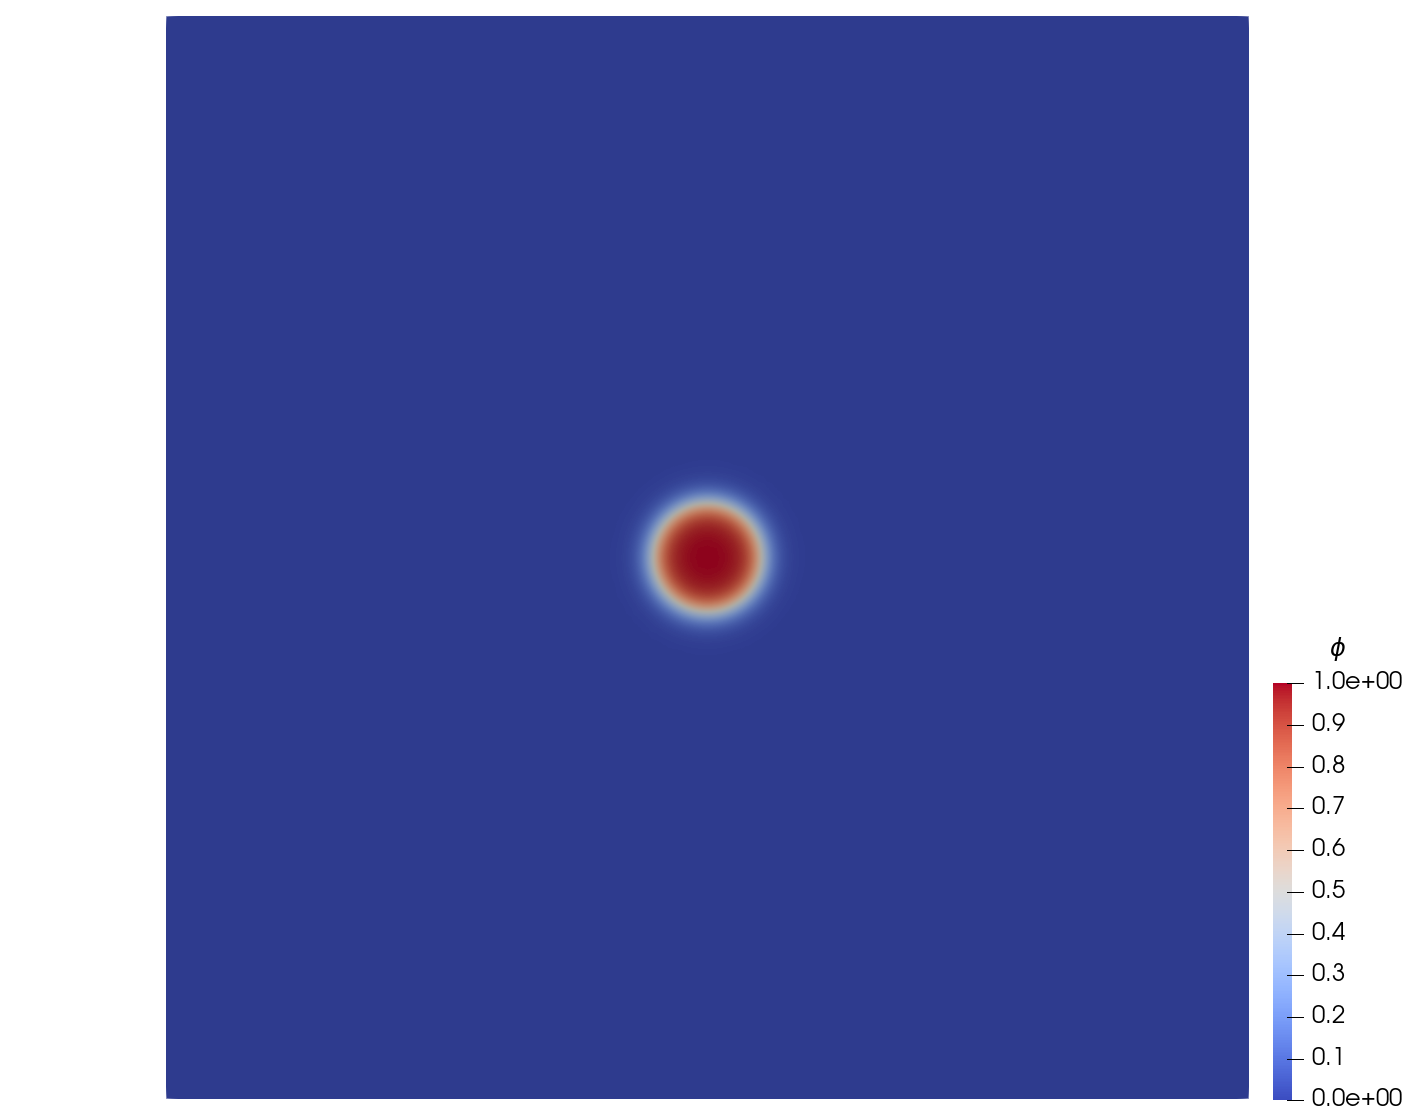
\includegraphics[scale=0.65]{t0_single_seed.PNG}
\par\end{centering}
\caption{Illustration of the $100 \times 100$ 2D computational domain and a diffuse-interface circular seed in the center. } \label{fig:t0_single_seed}
\end{figure}
\par\end{center}
%

\subsection{Explicit nucleation, multiple seeds at $t=0$}
%
The second part of the homogeneous nucleation benchmark problem focuses on the kinetics of nucleation using Avrami plots and compares them to the JMAK theory. To obtain reasonable statistics for these two parts, the simulation volume needs to be larger so it can encompass a larger number of smaller nuclei. We therefore increase the domain size to $500 \times 500$ units of length, and the driving force to $\Delta f = 1/(3 \sqrt{2})$, which corresponds to a critical radius of $r^*=2$. Random initial positions $\mathbf{r}_i$ of 25 supercritical seeds $i, i=1,\ldots,25$ are generated with $r_0=2.2r^*$ drawn from a uniform distribution on the $500\times500$ domain. The distribution of the phase field $\phi$ is the sum of the phase fields $\phi_i$ with profiles
\begin{equation}
    \phi_i(r)=\frac{1-\tanh\left(
    \frac{|\mathbf{r}-\mathbf{r}_i|-2.2r^*}{\sqrt{2}}
    \right)}{2}.
    \label{eqn:phitr_3}
\end{equation}
%
from the different seeds $i$. Overlaps between different seeds are eliminated by setting $\phi=1$ in all regions where the sums of $\phi_i >1$. After placing initial seeds and adjusting the initial phase field $\phi$ so that $\phi\leq1$ everywhere, the simulation is run up to total time $t=200$, at which time the whole domain is transformed to a solid ($\phi=1$).  This is repeated four times, each time with different random seeds, and the total free energy, time evolution of the solid fraction $X$, discrete particle count $N$  (the number of disjoint regions with $\phi=1$) are plotted for the five simulations, and Avrami plots are generated from the five simulations; from the Avrami plot the exponent $n$ is estimated and compared to the JMAK theory. A snapshot of the phase-field at $t=40$ is taken for one of the five runs.  %When adding a new seed $i$, we simply add the value of the new phase field $\phi_i$ values (given by the $\phi(r)$ profile (Eq.~\ref{eqn:phitr})) from the different seeds to the $\phi$ values already in the domain, and handle the possible overlaps by setting $\phi=1$ for all cells where $\phi>1$. Run the simulation until $t=300$. By this time the whole domain should be transformed to solid. Plot the total free energy, the time evolution of the transformed fraction and the discrete particle count, and make the Avrami plot. Then repeat the above procedures four more times with different random seeds for the nuclei positions.

This, and the third part below, of the explicit nucleation benchmark problem, involve a random number generator. Because different executions will in general generate different random numbers, specific individual solutions will in general not be reproduced. However, statistics such as the average slope of Avrami plots are reproducible.

\subsection{Explicit nucleation, multiple seeds at random times}
%
For the third part of the homogeneous benchmark problem, the computational domain is first expanded to $1000 \times1000$. Instead of inserting nuclei at fixed time $t = 0$ as in part two of the problem, in this case 100 random nucleation times $t_i$ are generated, $i=1,\ldots,100$, drawn from a uniform distribution in the interval $t_i \in [0, 600)$ with centers $\mathbf{r}_i$ drawn from a uniform distribution on the $1000\times1000$ domain. %for adding the 100 seeds to the simulation domain of size $1000 \times 1000$. 
The initial radii of the inserted nuclei are kept the same as those in the second part of the problem, 
\begin{equation}
    \phi_i(r)=\frac{1-\tanh\left(
    \frac{|\mathbf{r}-\mathbf{r}_i|-1.01r^*}{\sqrt{2}}
    \right)}{2}
\end{equation}
but now with a smaller driving force, 
\begin{equation}
\Delta f=1/(6\sqrt{2}).
\end{equation}
%
Again, $\phi$ is set to unity in regions of overlaps of nuclei. The simulations are run up to times $t=600$, and repeated for four more random initial conditions.  The total free energy plot the total free energy, the time evolution of the solid fraction $X$ and the discrete particle count $N$, are plotted as functions of time, and an  Avrami plot is generated for the five runs. Again, a snapshot of the phase-field at $t = 100$ is taken for one of the five runs. %{\bf Olle: what about overlaps of nuclei? Is $\phi$ set to 1 in regions of overlap?}

\subsection{Athermal heterogeneous nucleation}
%
For a benchmark problem on athermal heterogeneous nucleation, a surface with good wetting properties but of limited size is needed. In modeling of athermal heterogeneous nucleation, these nucleation surfaces represent small, flat, foreign particles which serve as nucleation sites. %In the usual scenario, they are the surfaces of small, flat foreign particles. 
In order to simplify the problem and to focus it on the athermal nucleation process rather than on technical issues with introducing foreign flat particles, we avoid adding additional boundaries (particles) to the problem formulation, and instead use one of the sides of a rectangular domain by making parts of it a good wetting surface. We use a parameter $\phi_0$ in Dirichlet boundary conditions on $\phi$ to determine the wetting properties of the bounding surface -- this corresponds to the ``Model B” approach described by Warren {\em et al}~\cite{warren2009phase}. %, i.e., to set the wetting properties via the parameter $\phi_0$ used in the Dirichlet boundary condition $\phi=\phi_0$ along the surface. 
This ``Model B" approach has two advantages: (i) it is very simple to implement, and (ii) if we set $\phi_0$ large enough, a surface spinodal would occur, i.e., a solid phase will automatically appear at and grow from the surface, so we can eliminate the effort of inserting an appropriate seed in the beginning of the simulation.

The goal of this problem is to explore the behavior around the free growth limit, which, in our 2D setting, is the half-circular configuration of solid on top of a straight surface of length $2r_0$, where $r_0$ is the radius of the homogeneous nucleus corresponding to the given driving force (Eq. ~\ref{eqn:trc}). To define the problem, the undercooling is set to $\Delta f_0 = 1/(30 \sqrt{2})$, which corresponds to a critical radius $r^*=10$, and a simulation domain of width 40 units and height 20 units is used. As shown in Fig.~\ref{fig:t0_athermal_thick}, Dirichlet boundary conditions on the bottom side are defined by setting $\phi_{0}=0.9$ along the middle part of length 20 of the boundary and $\phi_{0}=0$ outside. Starting from $\phi=0$ everywhere else, the simulation is run for times $t$ up to $t = 6500$, and the transformed fraction $X$ is plotted as function of time $t$. The simulation is repeated with varying undercooling $\Delta f=0.98\Delta f_0$, $\Delta f=1.02\Delta f_0$, $\Delta f=1.04\Delta f_0$, respectively. %Then compare the results. 
An additional convergence tests with respect to spatial and temporal resolution is added for the solid fraction change when $r_0=1.1r^*$: keep halving the linear dimension of the mesh and calculate the L2 error at time $t=800$ between consecutive meshes until the L2 error is less than 0.25.

%
\begin{center}
\begin{figure} 
\begin{centering}
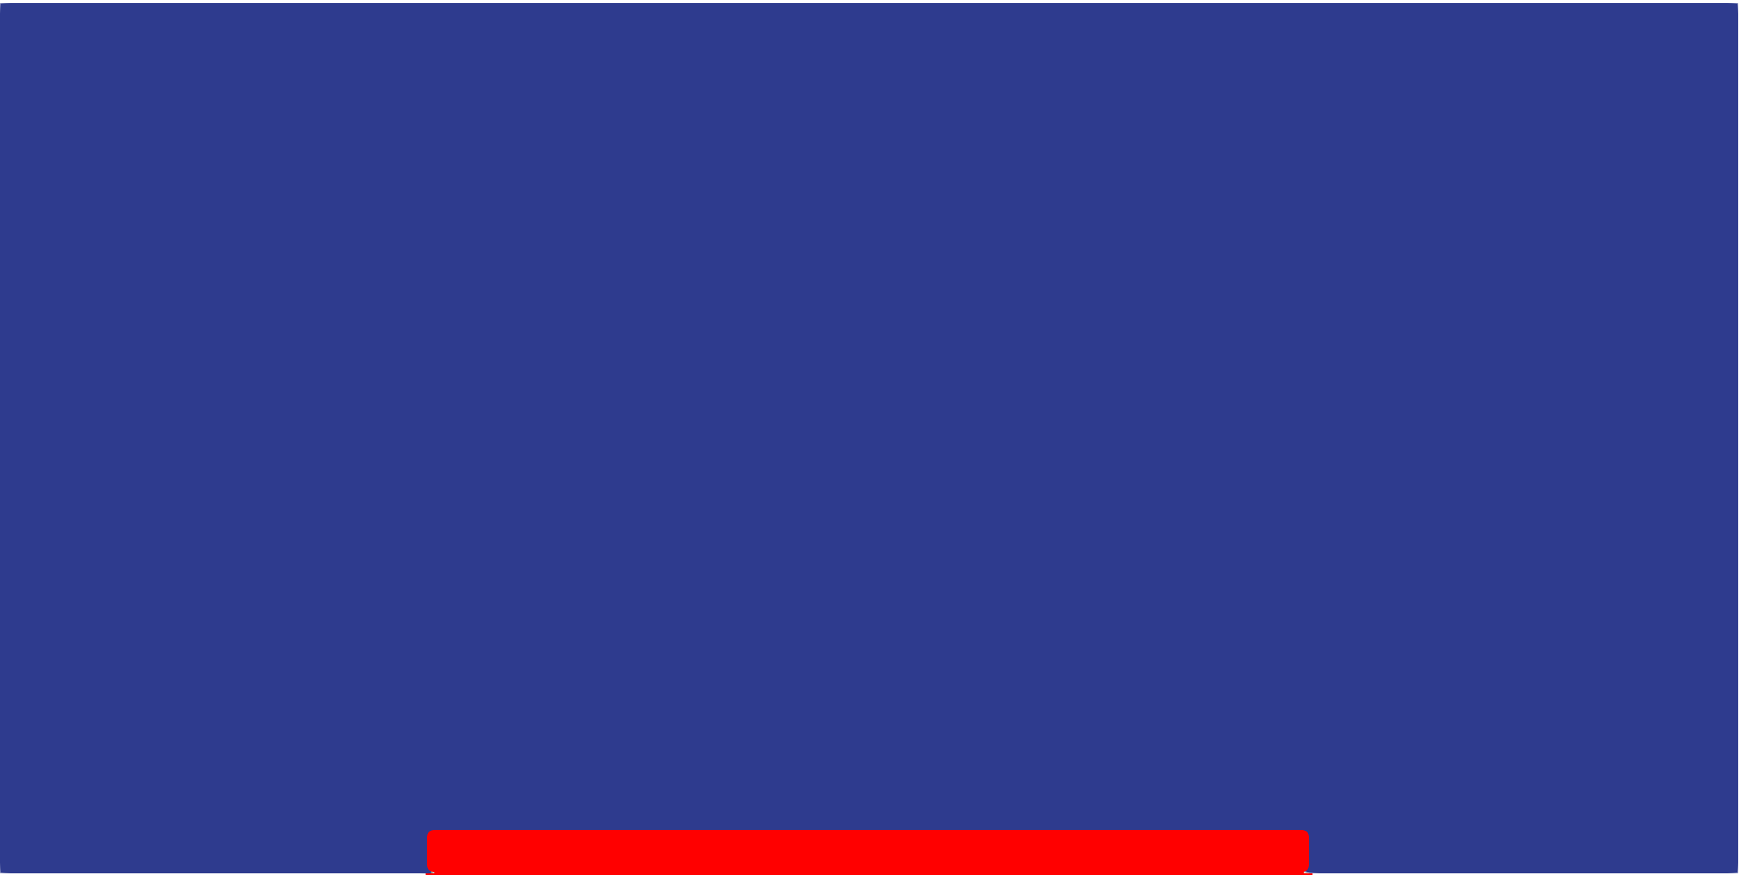
\includegraphics[scale=0.50]{t0_athermal_thick.PNG}
\par\end{centering}
\caption{Illustration of the $40 \times 20$ 2D computational domain with Dirichlet boundary conditions on the bottom side. The red line represents the middle part of the boundary of length 20 where $\phi_{0}=0.9$, $\phi_{0}=0$ elsewhere.} \label{fig:t0_athermal_thick}
\end{figure}
\par\end{center}
%

\section{Numerical methods}

We use an application within the MOOSE framework~\cite{gaston2014continuous,gaston2015physics} for our simulations, as we have done for previous benchmark problems. In addition, we have compared the solutions obtained with MOOSE with three other codes or methods. One of them is a bespoke finite difference method, and the others are based on finite element (PRISMS-PF)~\cite{dewitt2020prisms} or finite volume methods (FiPy)~\cite{guyer2009fipy}. All solutions are uploaded to the PFHub website~\cite{wheeler2019pfhub} \url{https://pages.nist.gov/pfhub/}. %provided via finite element applications including MOOSE framework \cite{gaston2014continuous,gaston2015physics}, PRISM \cite{} and Fipy \cite{}.  We use these methods in this work to provide four sets of solution data on the benchmark website as a basis for comparison with the results of other numerical solution methods and implementations.

%The finite difference code that is used to solve the nucleation benchmark problems applies forward Euler time stepping. For the first single seed homogeneous nucleation and the fourth athermal heterogeneous nucleation benchmark problem, the time step is $\Delta t=0.01$, and the spatial resolution is $\Delta x=\Delta y=0.4$ with periodic boundary conditions. In particular, four different spatial resolutions ($\Delta x=0.8, 0.4, 0.2, 0.1$) are used for the convergence test when plotting the solid fraction versus time for the first problem $r_0=1.01r^*$ case. The corresponding time steps are set to $\Delta x=0.04, 0.01, 0.01/4, 0.01/16$ for the stability criterion. %Two different spatial resolutions ($\Delta x=0.4, 0.2$) are used for the convergence test when plotting the solid fraction versus time for the fourth problem $\Delta f=1.1\Delta f_0$ case.
%For the second and third multiple seed homogeneous nucleation benchmark problem, the time step and spatial resolution are adjusted to $\Delta t=0.01$, $\Delta x=0.04$, respectively in order to make the simulation faster.

The computational domains created by the MOOSE application are meshed using square, four-node quadrilateral elements. First-order Lagrange shape functions are employed for the order parameter $\phi$. The system of nonlinear equations is solved with the full Newton method that uses the single-matrix preconditioning with the additive Schwarz preconditioner and ILU sub-preconditioning. The second backward differentiation formula (BDF2) time integration scheme is applied. The simulations are solved with a nonlinear relative tolerance of $1\times10^{-6}$ and a nonlinear absolute tolerance of $1\times10^{-9}$. A maximum of ten nonlinear iterations per solve, and a maximum of 50 linear iterations, are specified. To improve computational efficiency, adaptive meshing and adaptive time stepping are used. The initial time step $\Delta t$ is set to 0.01, and the time step is allowed to grow by 5\%. For the single-seed homogeneous nucleation part of the first problem, the mesh contains $64\times64$ elements. This translates to an element size of $\Delta x=1.5625$. A single element can be refined up to four times for adaptive meshing. Thus the finest part of the mesh has elements with size $\Delta x=0.098$. The convergence test for the solid fraction change in the $r_0=1.01r^*$ case is done by four simulations with different fixed spatial resolutions ($\Delta x=0.8, 0.4, 0.2, 0.1$), and compared with applying the adaptive mesh. For the second and third parts of the first problem, the mesh contains $160\times160$, and $320\times320$ elements, respectively, which result in the same spatial resolution, $\Delta x=3.125$, and the finest part of the mesh has elements with size $\Delta x=0.195$. For the second problem on athermal nucleation, the mesh contains $100\times50$ elements, which gives an element size of $\Delta x=0.4$. With the adaptive meshing, the size of the smallest element is $\Delta x=0.025$. 
Five different spatial resolutions ($\Delta x=0.4, 0.2, 0.1, 0.05, 0.025$) are used for the convergence test when plotting the solid fraction versus time for the $\Delta f=1.1\Delta f_0$ case. We also compare the results with the simulation using adaptive meshing.



\section{Results and discussion}

In this section, we discuss the example solutions and metrics obtained from them. We also study error and convergence behavior for the $r_0=1.01r^*$ case in the single seed homogeneous nucleation problem and the $\Delta f=1.1\Delta f_0$ case in the athermal heterogeneous nucleation problem. Furthermore, we discuss some peculiar issues that may arise in solving these benchmark problems.


\subsection{Explicit nucleation, single seed}

For this problem we mainly look into how the initial radius of the inserted seed determines whether the nucleation is going to happen or not. We choose the total free energy of the system and the solid fraction as metrics with which to compare simulation results. 

Fig.~\ref{fig:free_energy_single_seed} shows the total free energy of the system, and Fig.~\ref{fig:solid_fraction_single_seed} shows the solid fraction changes over time. When the initial radius of the seed is smaller than the critical radius ($r_0=0.99r^*$), based on classical nucleation theory the quantity $d\Delta G/dr$ in Eq.~\ref{eqn:ddeltaGdr} is positive. That means that it is energetically more favorable for the system to decrease the size of the nucleus. As a result, the total free energy (black dashed line in Fig.~\ref{fig:free_energy_single_seed}) and the solid fraction (black dashed line in Fig.~\ref{fig:solid_fraction_single_seed}) both decrease over time. The inserted seed shrinks and around $t=90$, it fully dissolves into the liquid. The solid fraction drops to zero and the total free energy of the system stops decreasing. Nucleation does not happen in this case. 
%COMMENT there's too much discussion of the free energy decreasing.  Our equations require this. It's both a sanity check and a benchmarking tool, it's not technically interesting beyond that
On the other hand, when the initial radius of the seed is larger than the critical radius ($r_0=1.01r^*$), $d\Delta G/dr$ in Eq.~\ref{eqn:ddeltaGdr} is negative, and it is energetically favorable for the system to increase the size of the nucleus. This explains why  although the total free energy (blue dash-dot line in Fig.~\ref{fig:free_energy_single_seed}) is still decreasing, the solid fraction (blue dash-dot line in Fig.~\ref{fig:solid_fraction_single_seed}) is now increasing over time. The inserted seed grows and nucleation occurs in this case. We note that with no fluxes entering or leaving the system, the total energy is necessarily monotonically non-increasing.

When the initial radius of the seed is equal to the critical radius ($r_0=1.00r^*$),  $d\Delta G/dr$ in Eq.~\ref{eqn:ddeltaGdr} is equal to zero, and the system is in an unstable equilibrium state. Therefore, the total free energy (red solid line in Fig.~\ref{fig:free_energy_single_seed}) stays approximately constant. Ideally, the solid fraction would also remain constant. The small changes in the calculated solid fraction (red solid line in Fig.~\ref{fig:solid_fraction_single_seed}) when $t$ is large are due to numerical errors that accumulate with time. Because the system is unstable, small errors will then eventually lead to growth or shrinkage of the nucleus.

The convergence test for the solid fraction change for the case $r_0=1.01r^*$ is shown in Fig.~\ref{fig:convergence_single_seed}. We choose $r_0=1.01r^*$ for the convergence test because the system is very sensitive when $r_0=1.00r^*$, and small numerical errors can result in exponential growth of error. On the other hand, if $r_0$ is too far from $r^*$, numerical integration is rather robust and convergence is readily achieved. Figure~\ref{fig:convergence_single_seed} clearly shows that the mesh resolution has a significant effect on the time-evolution of the solid fraction. When the mesh size is large with low resolution, i.e., $\Delta x=0.8$, only a small increase in solid fraction is observed before $t=200$, and the nucleus grows slowly. When we refine the mesh to increase the spatial resolution, the solid fraction increases more rapidly. The calculated L2 error between simulations with consecutive meshes $\Delta x=0.4$ and $\Delta x=0.2$ is 2.78, and that between mesh sizes of $\Delta x=0.2$ and $\Delta x=0.1$ is 0.69, which indicates that the results from the two meshes are similar. Further increases in the mesh resolution would significantly improve the accuracy of the simulation results. This is also indicated in Fig.~\ref{fig:convergence_single_seed} where the curves of $\Delta x=0.2$ and $\Delta x=0.1$ are indistinguishable. The adaptive mesh behaves similarly to the refined fixed mesh. We thus treat the solution generated with $\Delta x=0.1$ as a gold standard solution for comparison with the results of other numerical solution methods and implementations. 

%
\begin{center}
\begin{figure} 
\begin{centering}
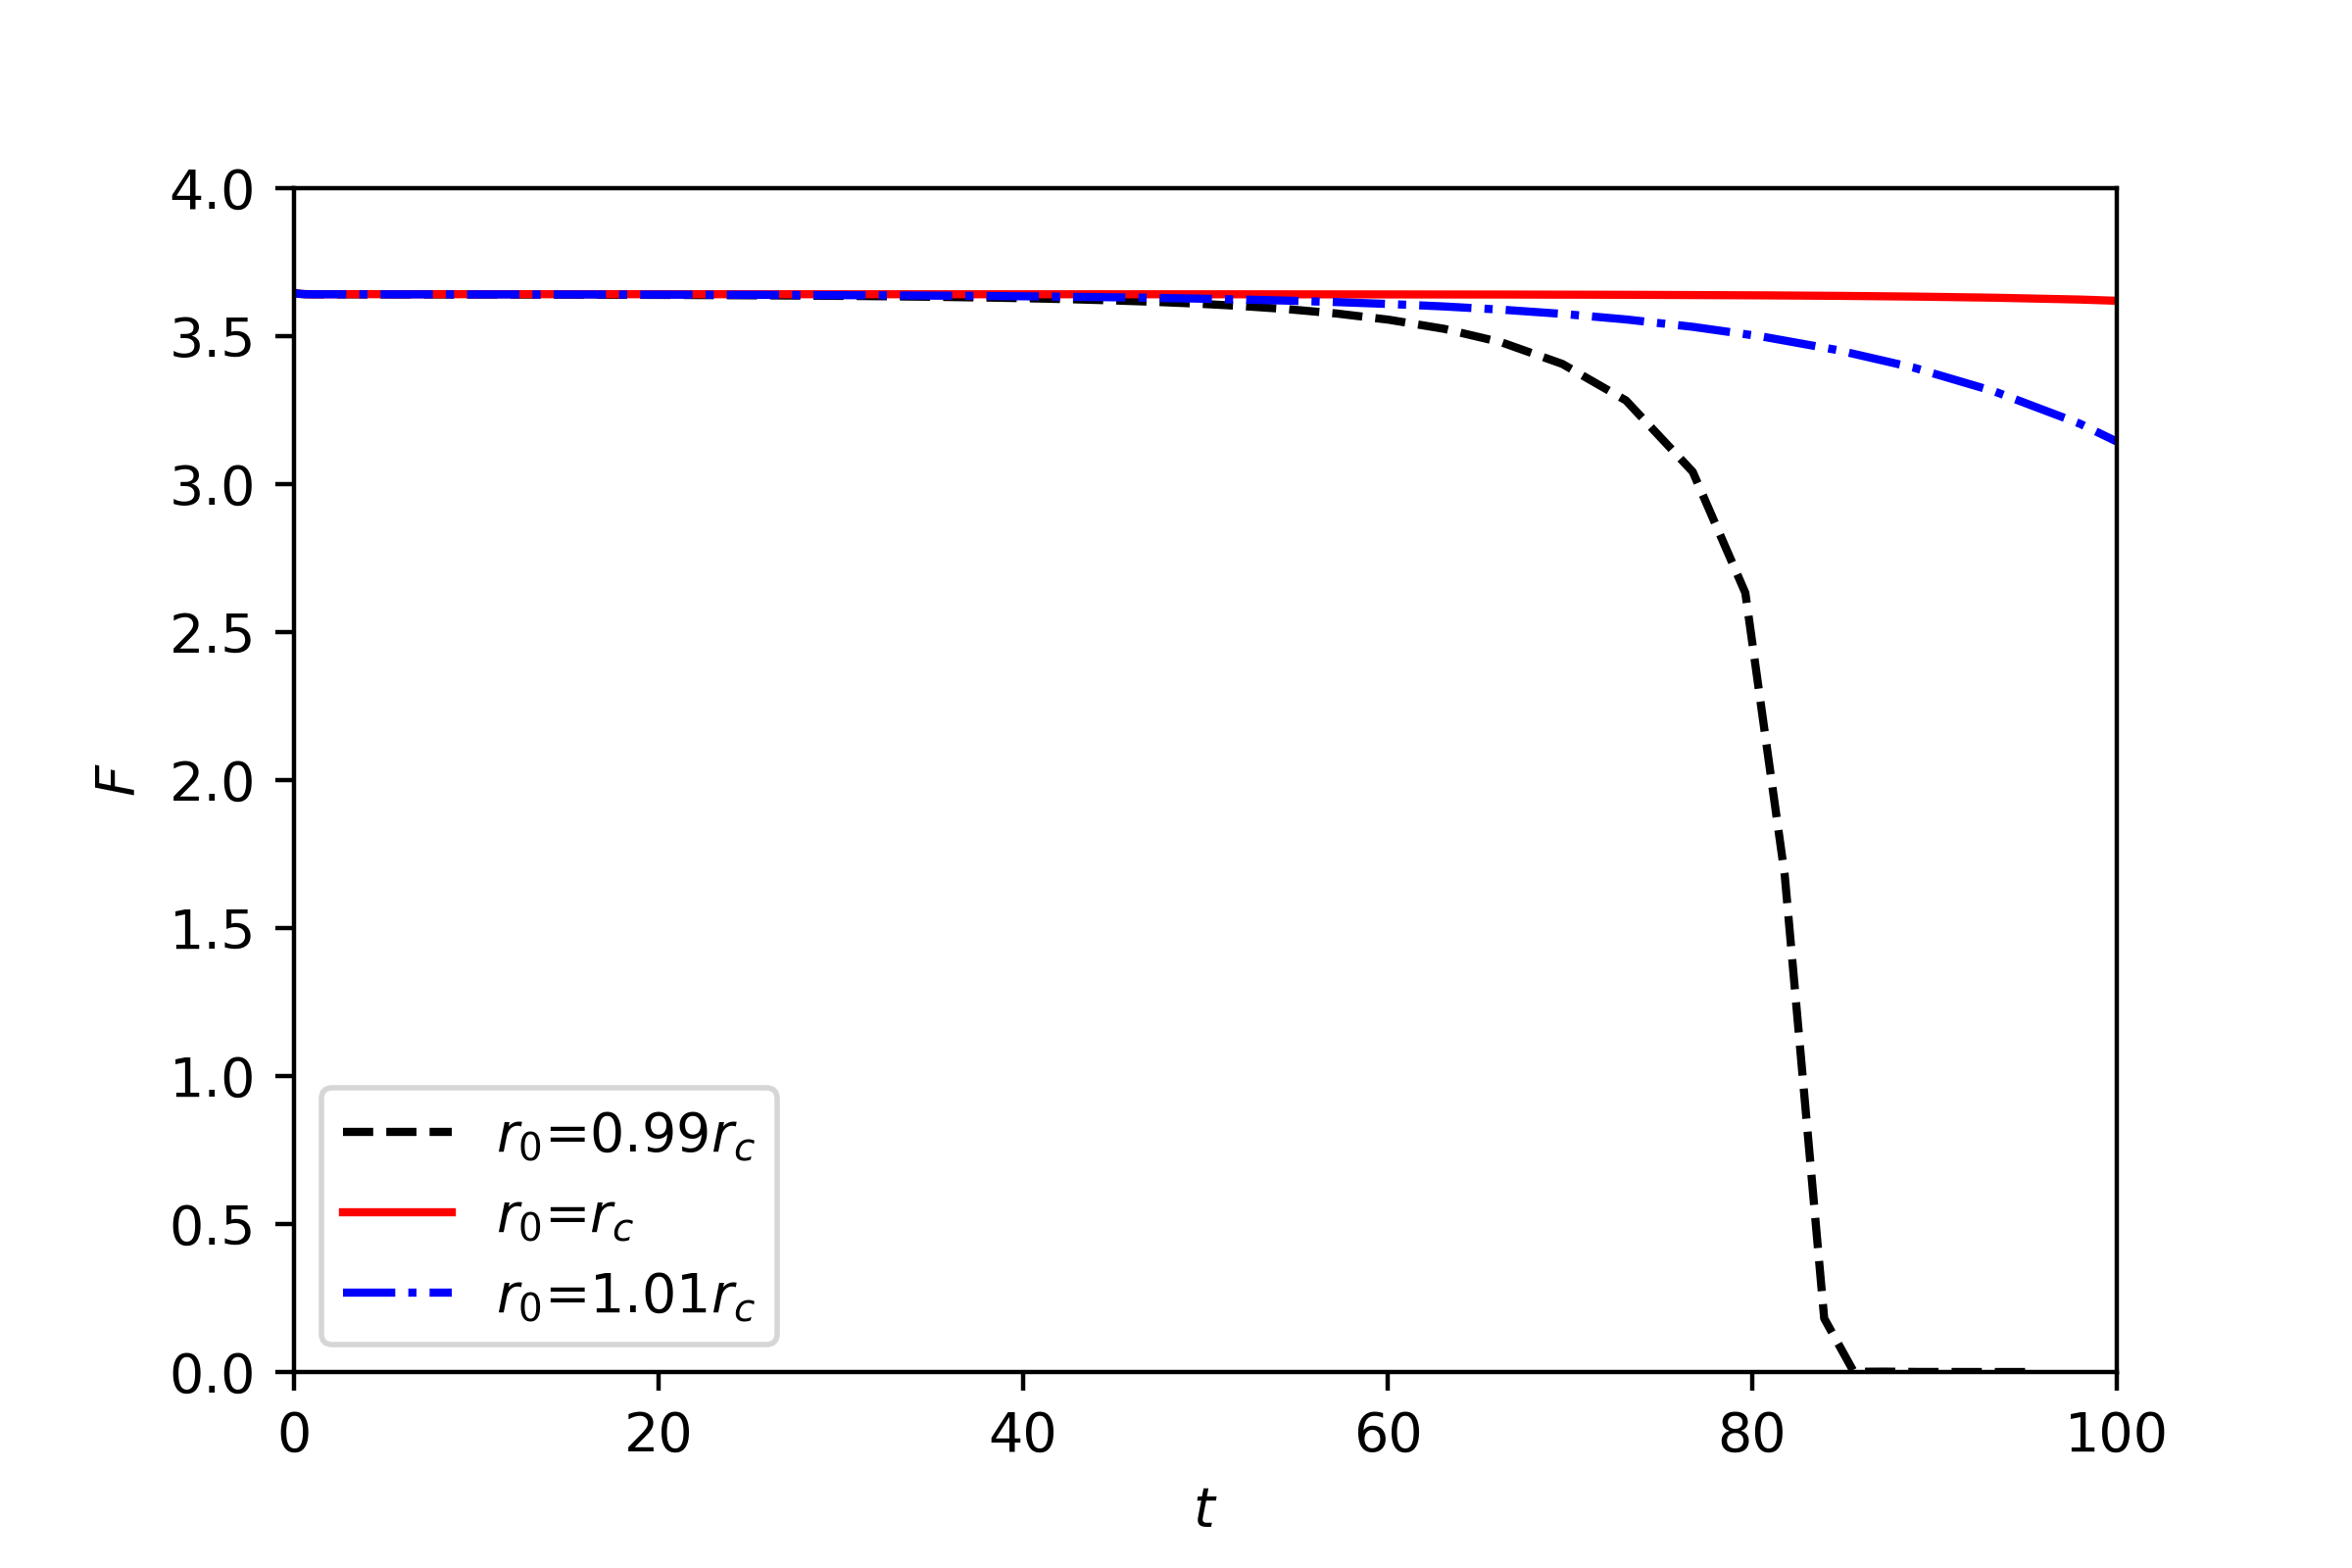
\includegraphics[scale=0.65]{free_energy_single_seed.PNG}
\par\end{centering}
\caption{The total free energy evolution of the single seed homogeneous nucleation.} \label{fig:free_energy_single_seed}
\end{figure}
\par\end{center}
%
%
\begin{center}
\begin{figure} 
\begin{centering}
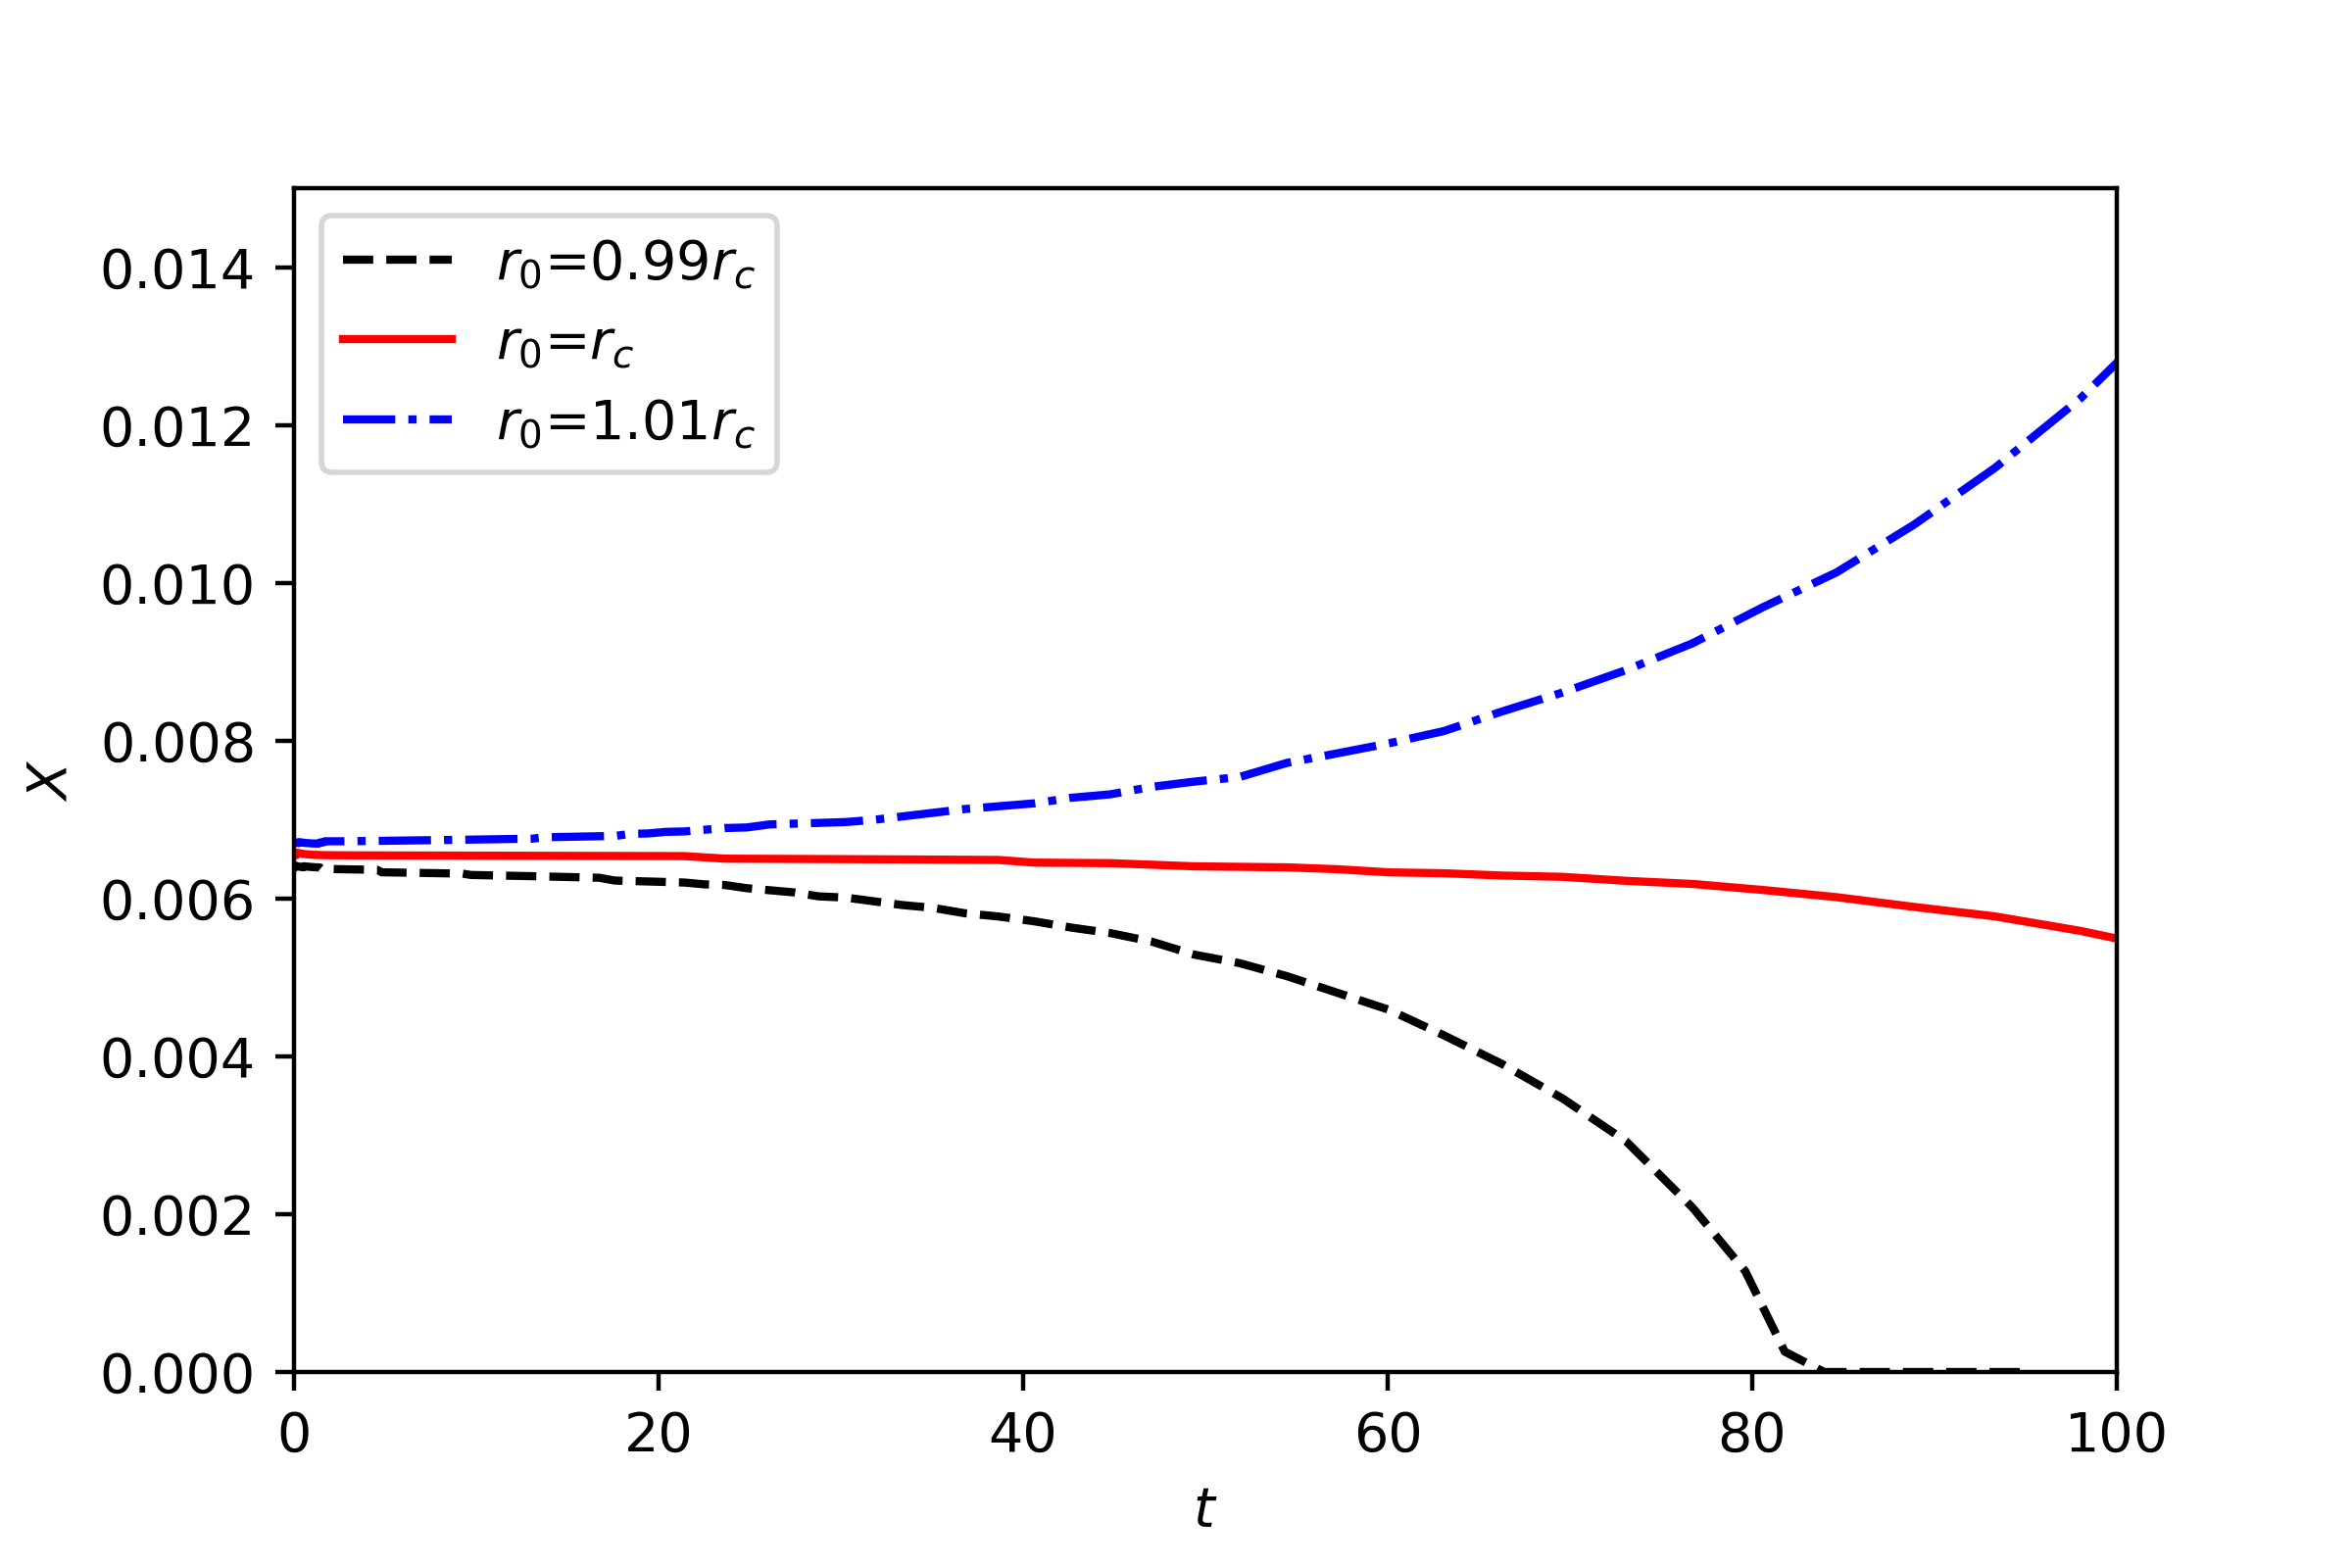
\includegraphics[scale=0.65]{solid_fraction_single_seed.PNG}
\par\end{centering}
\caption{The solid fraction of the single seed homogeneous nucleation.} \label{fig:solid_fraction_single_seed}
\end{figure}
\par\end{center}
%
%
\begin{center}
\begin{figure} 
\begin{centering}
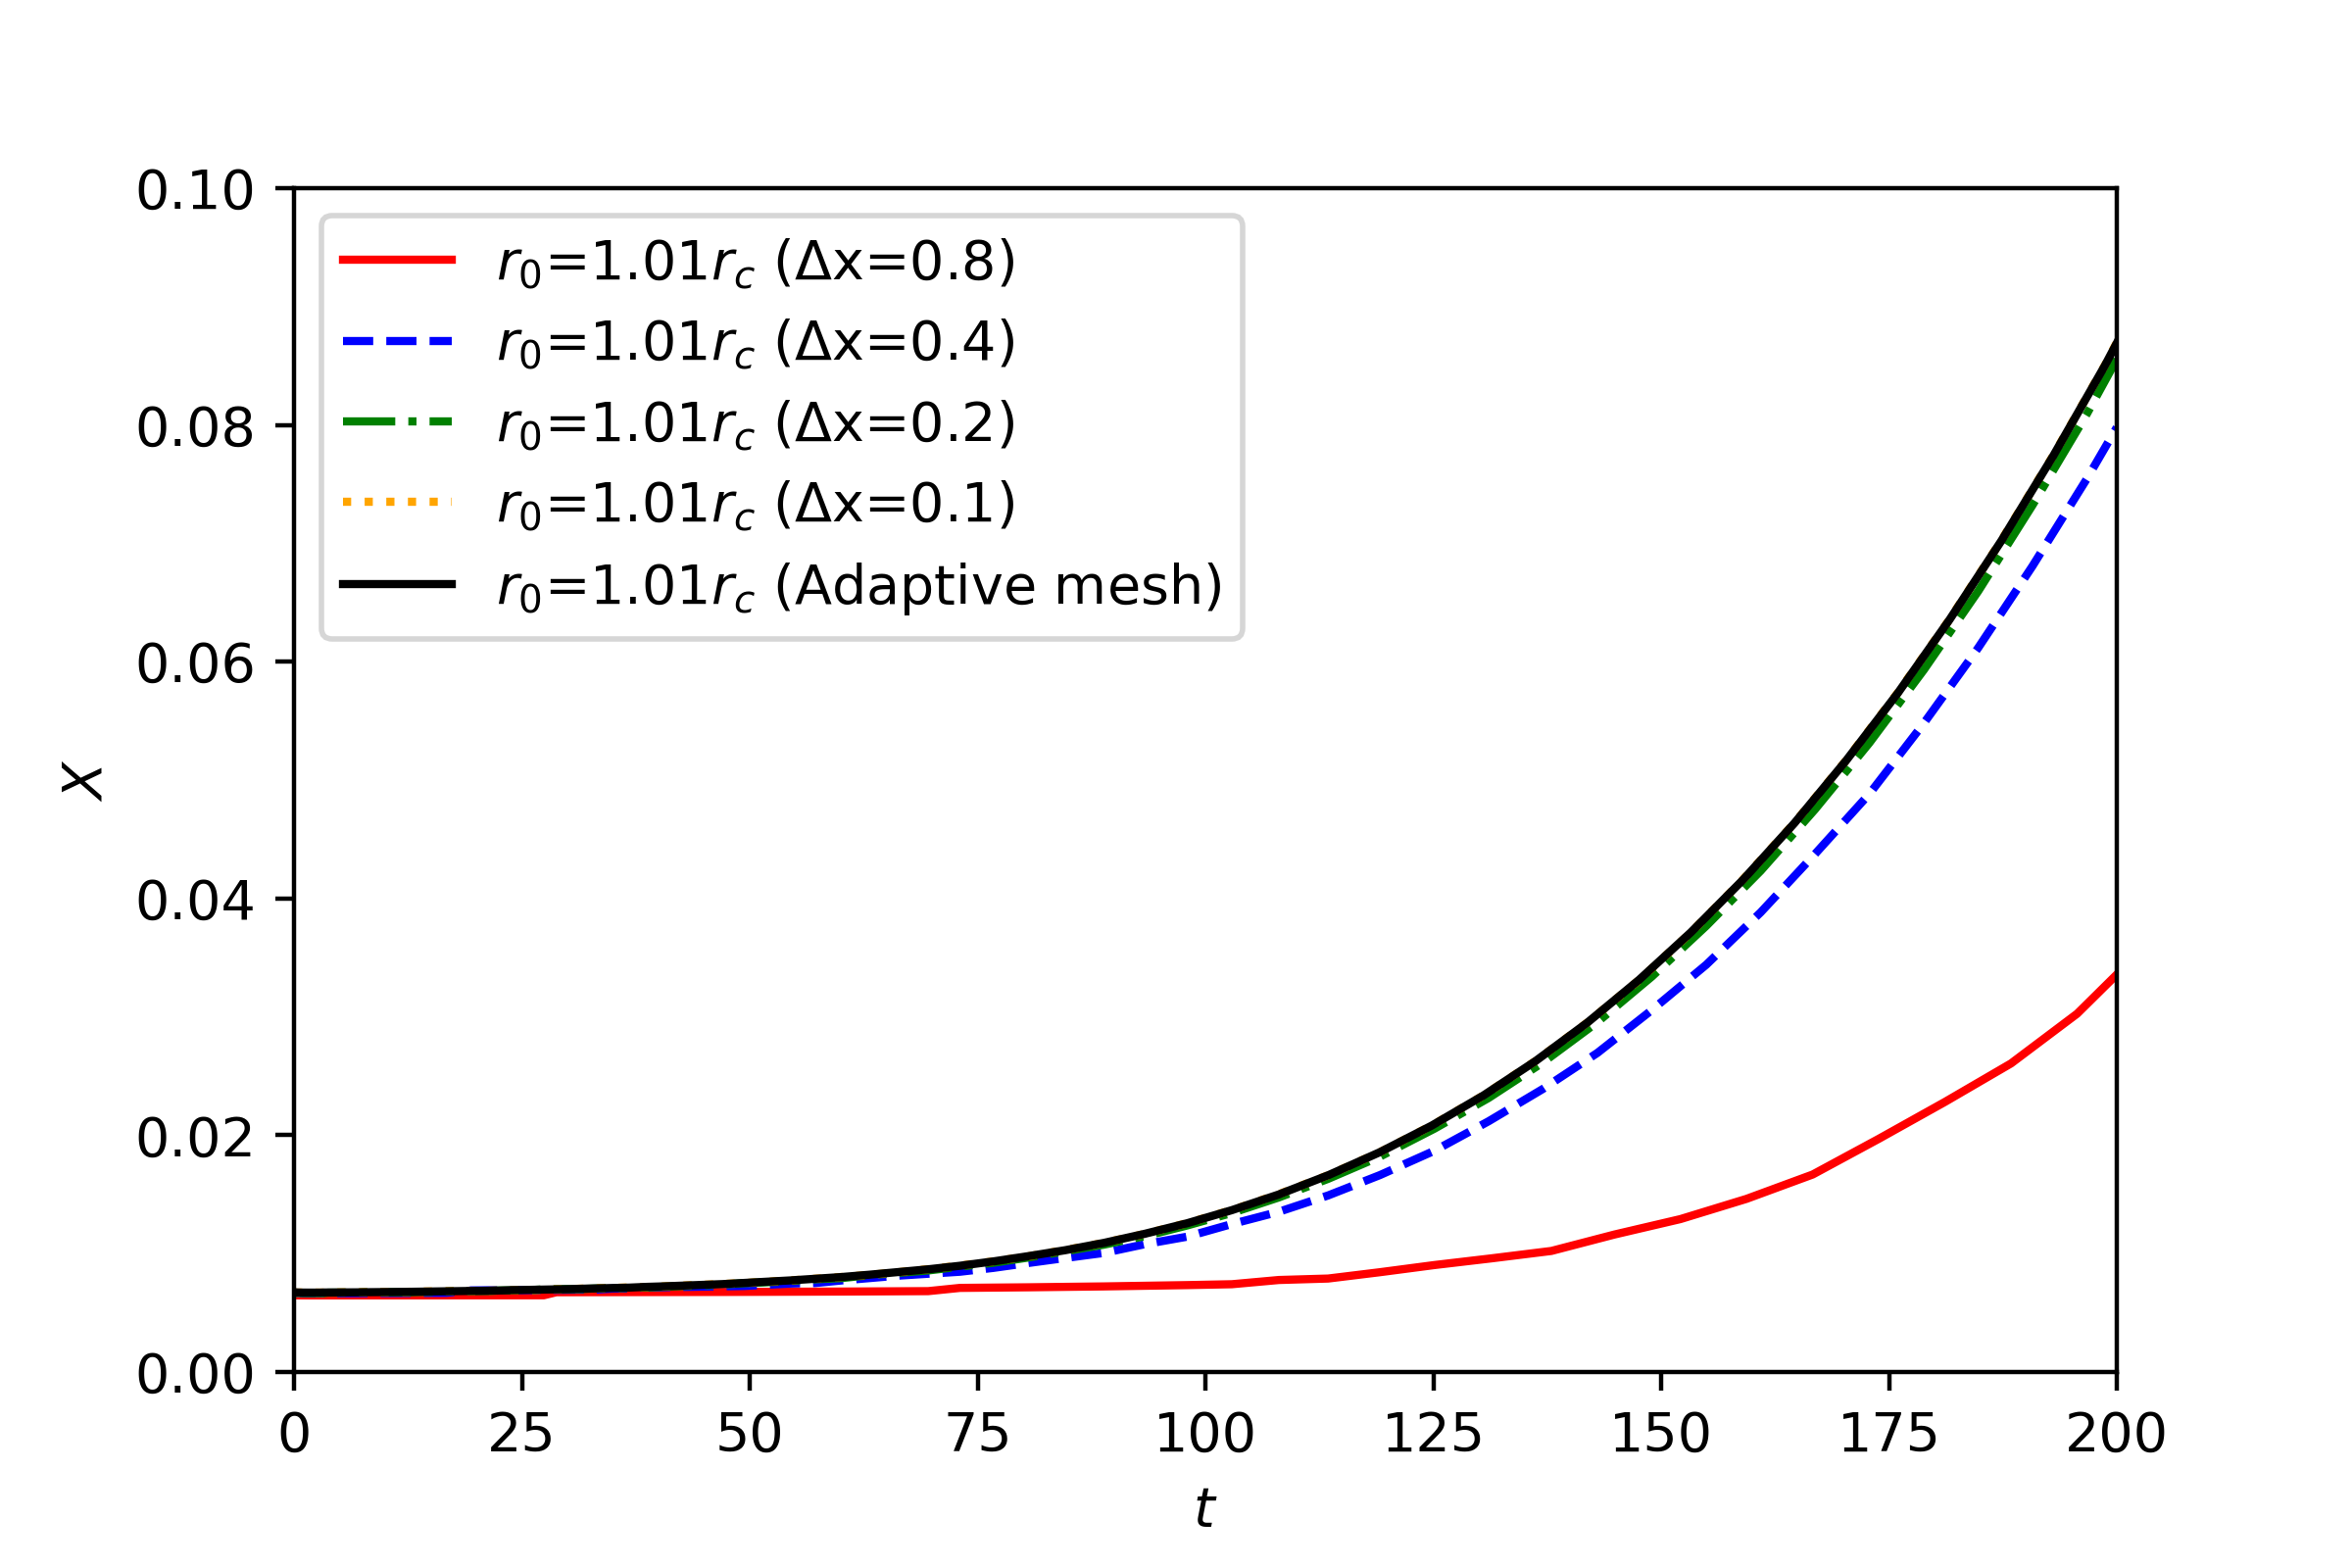
\includegraphics[scale=0.65]{convergence_single_seed.PNG}
\par\end{centering}
\caption{Convergence test for the solid fraction change for $r_0=1.01r^*$.}\label{fig:convergence_single_seed}
\end{figure}
\par\end{center}
%

\subsection{Explicit nucleation, multiple seeds at $t=0$}

For this part of the homogeneous nucleation benchmark problem we mainly look into the nucleation behavior when multiple seeds are inserted at $t=0$. Besides the total free energy of the system and the solid fraction, we also add the number of discrete particles and the Avrami plot as metrics. Figures~\ref{fig:free_energy_multiple_seed_t0}, ~\ref{fig:solid_fraction_multiple_seed_t0}, ~\ref{fig:particle_count_multiple_seed_t0},~\ref{fig:avarmi_plot_multiple_seed_t0} depict the calculated total free energy of the system, solid fraction, number of discrete particles and the Avrami plot for the multiple-seed homogeneous nucleation at $t=0$, respectively. A snapshot of the phase-field domain at $t=40$ is taken and shown in Fig.~\ref{fig:t40_multiple_seed_t0}. %{\bf Olle: was this part of the problem formulation?}

In all five cases with different random nuclei positions, the total free energy is decreasing monotonically, as shown in Fig.~\ref{fig:free_energy_multiple_seed_t0}, as should be the case.  Since the initial radius for the nuclei is larger than the critical radius, we expect to see an increase for the solid fraction over time, and the nuclei should grow and eventually fill up the entire simulation volume. This is indeed the case, as shown in Fig.~\ref{fig:solid_fraction_multiple_seed_t0}. The solid fraction increases with time in an S-shaped curve with a short tail. The short tail means that the early stage of the nucleation with a low transformation rate is short, since all the nuclei are inserted and ready to grow at time $t=0$. For most cases, the number of discrete particles starts at 25 since we insert 25 seeds at $t=0$. However, the number of discrete particles can be smaller, e.g., 24 or even less, if two or more inserted seeds overlap. The number of discrete particles also decreases monotonically and finally drops to unity at some time between $t=75$ and $100$, which indicates that the nuclei have merged into one large particle. The snapshot in Fig.~\ref{fig:t40_multiple_seed_t0} is used as an illustration, showing twelve discrete particles at $t=40$ which is the outcome of two or more particles merging. Notice that the seeds in Fig.~\ref{fig:t40_multiple_seed_t0} have equal size since they are inserted at the same time $t=0$. The nucleation kinetics is compared with the JMAK theory by making the Avrami plots in Fig.~\ref{fig:avarmi_plot_multiple_seed_t0} and extracting the exponent $n$. %As discussed in the previous section, the Avrami plots come from the JMAK equation (Eq.~\ref{eqn:Xt}). 
When all the nucleation events happen at $t=0$, the slope of the Avrami plot should be close to the dimension of the simulation domain, which is 2.0 in this case. Ideally the size of the system should be infinite for the JMAK theory to hold, but this is not realistic in our simulation. We fit a straight line to the data ranging from $1.1 < \log t < 2.1$. The average slope of the fitted line for the five runs is $n=2.01$, and the variance is $0.001$ %{\bf Olle: need to have better statement for the exponent - which regions was/were used for fit, and what is the result of the fit with one decimal place?}. NEED TO LOOK INTO THE REASON FOR THIS!! 
In addition, we see that the Avrami plots of the five runs with different initial random positions overlap with each other very well. This indicates that the initial positions of the nuclei have little influence on the nucleation kinetics. 
%
\begin{center}
\begin{figure} 
\begin{centering}
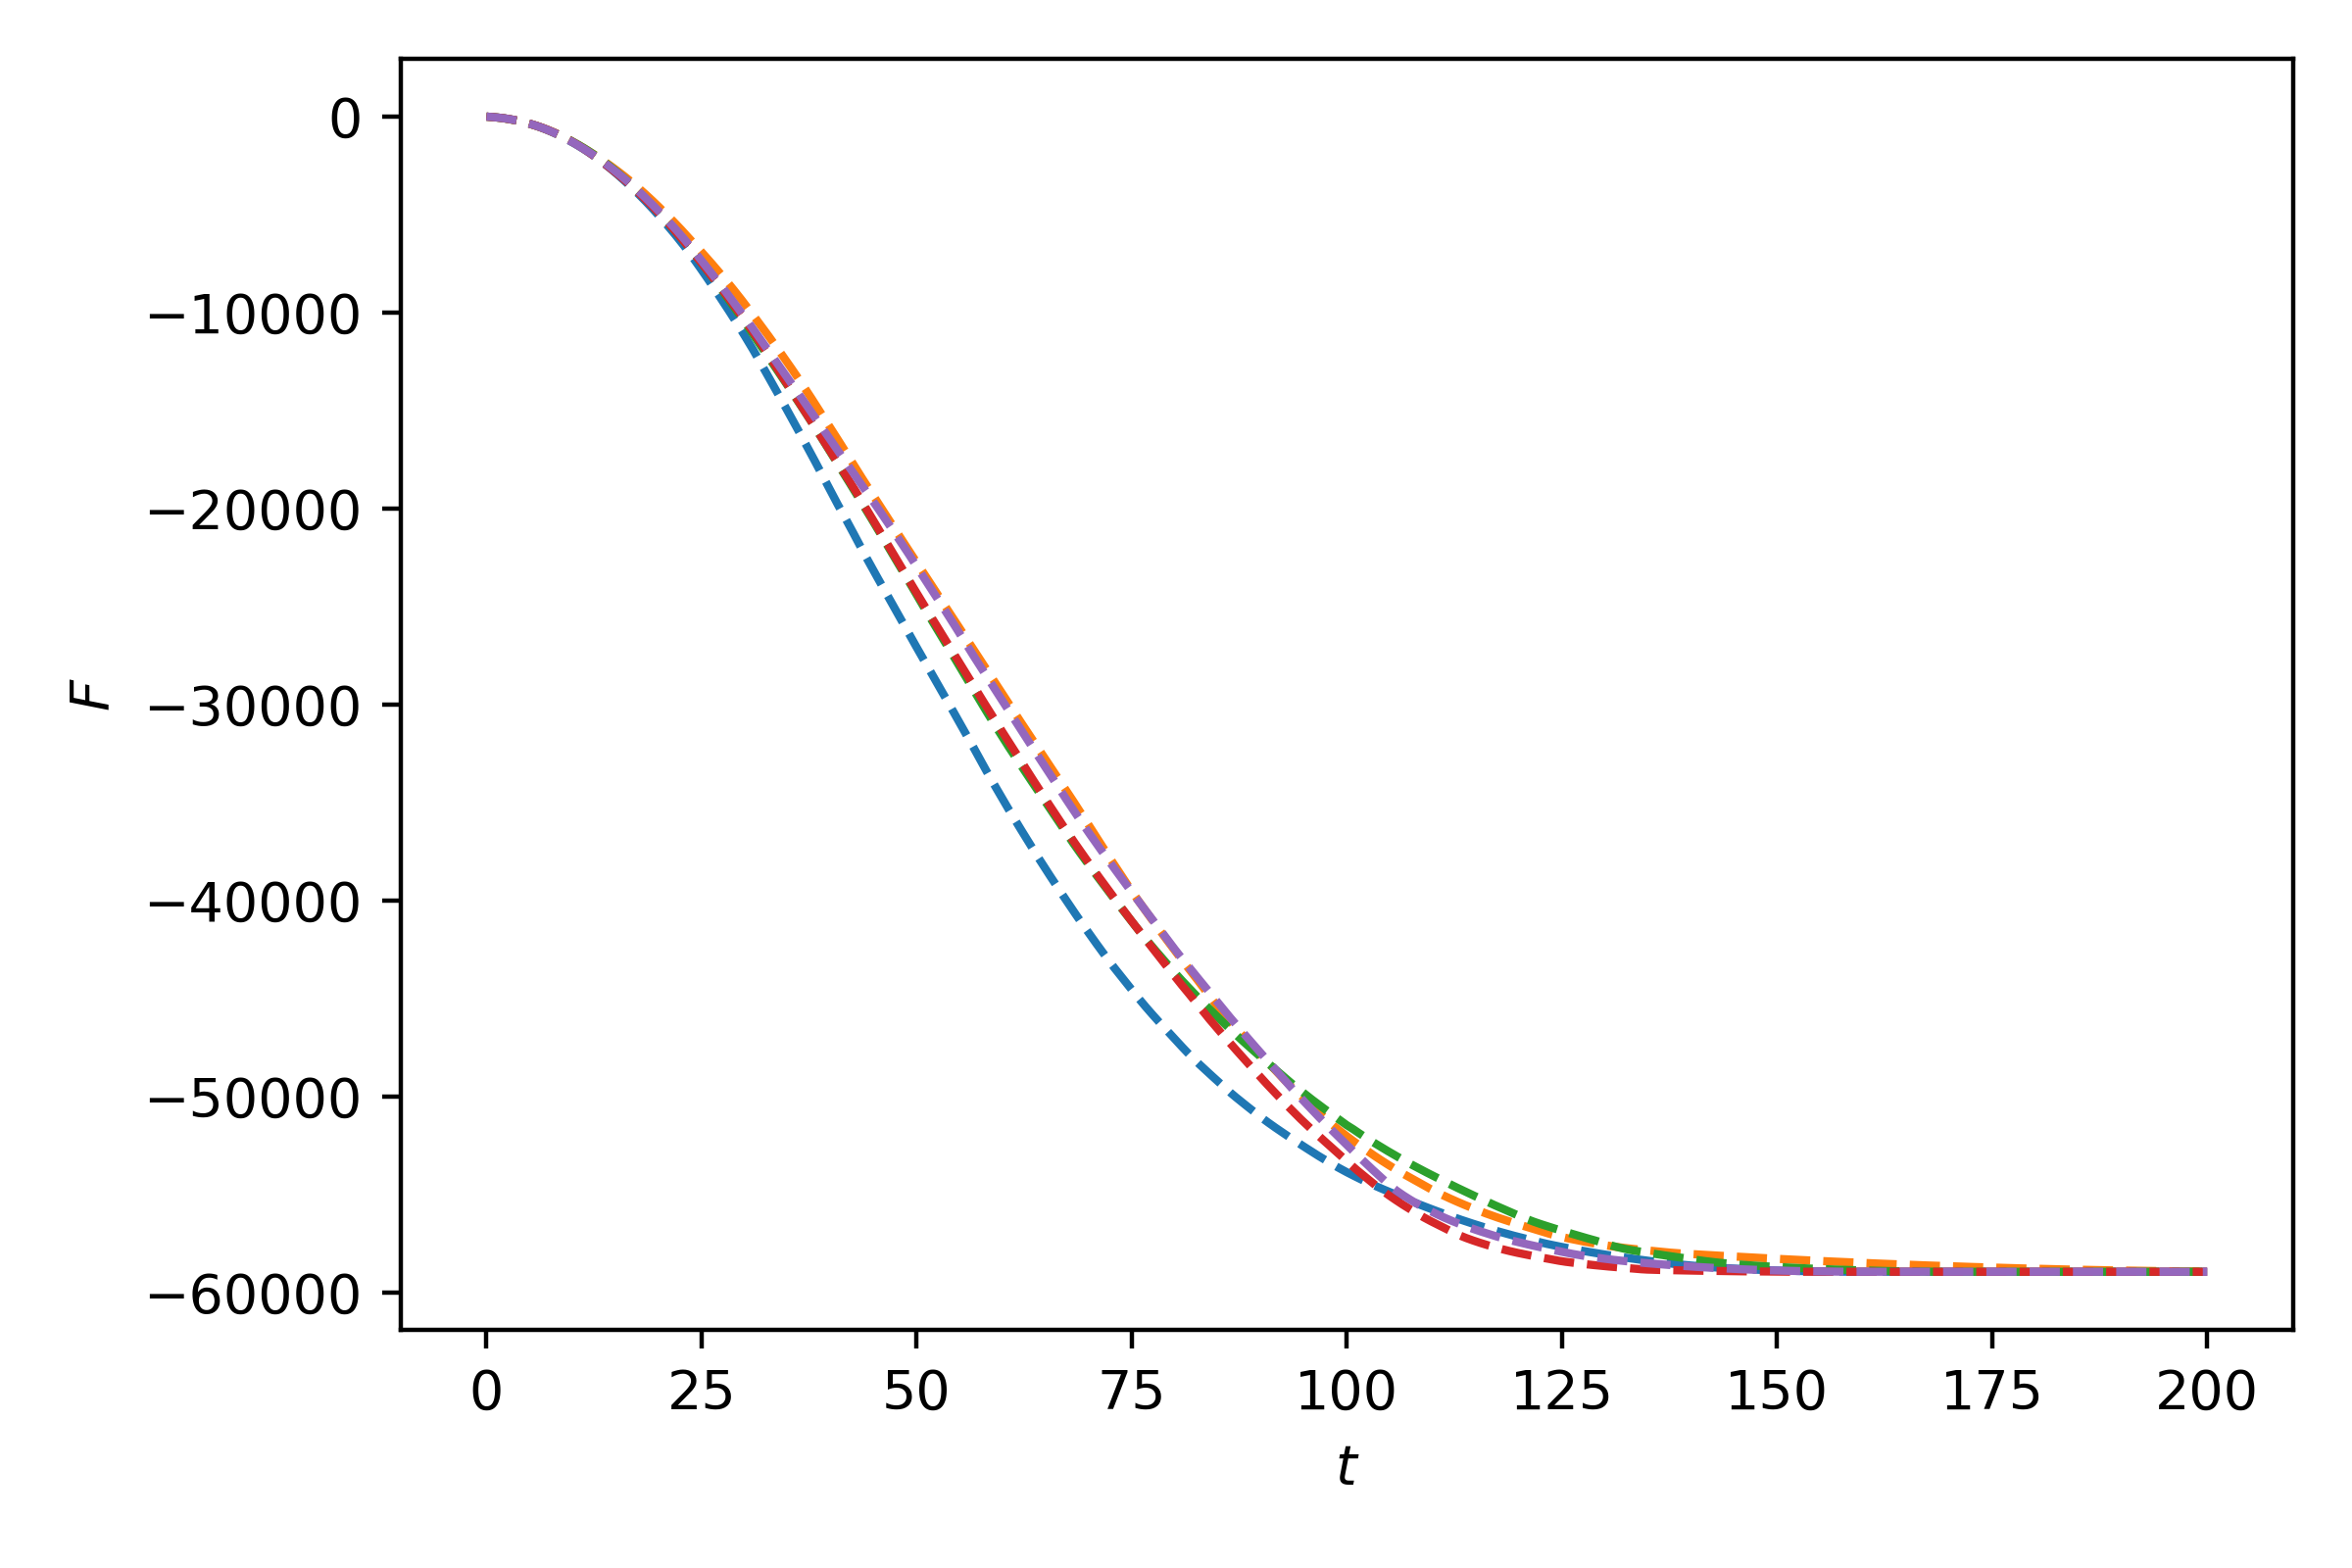
\includegraphics[scale=0.65]{free_energy_multiple_seed_t0.PNG}
\par\end{centering}
\caption{The total free energy evolution of the multiple seed homogeneous nucleation at $t=0$.} \label{fig:free_energy_multiple_seed_t0}
\end{figure}
\par\end{center}
%
\begin{center}
\begin{figure} 
\begin{centering}
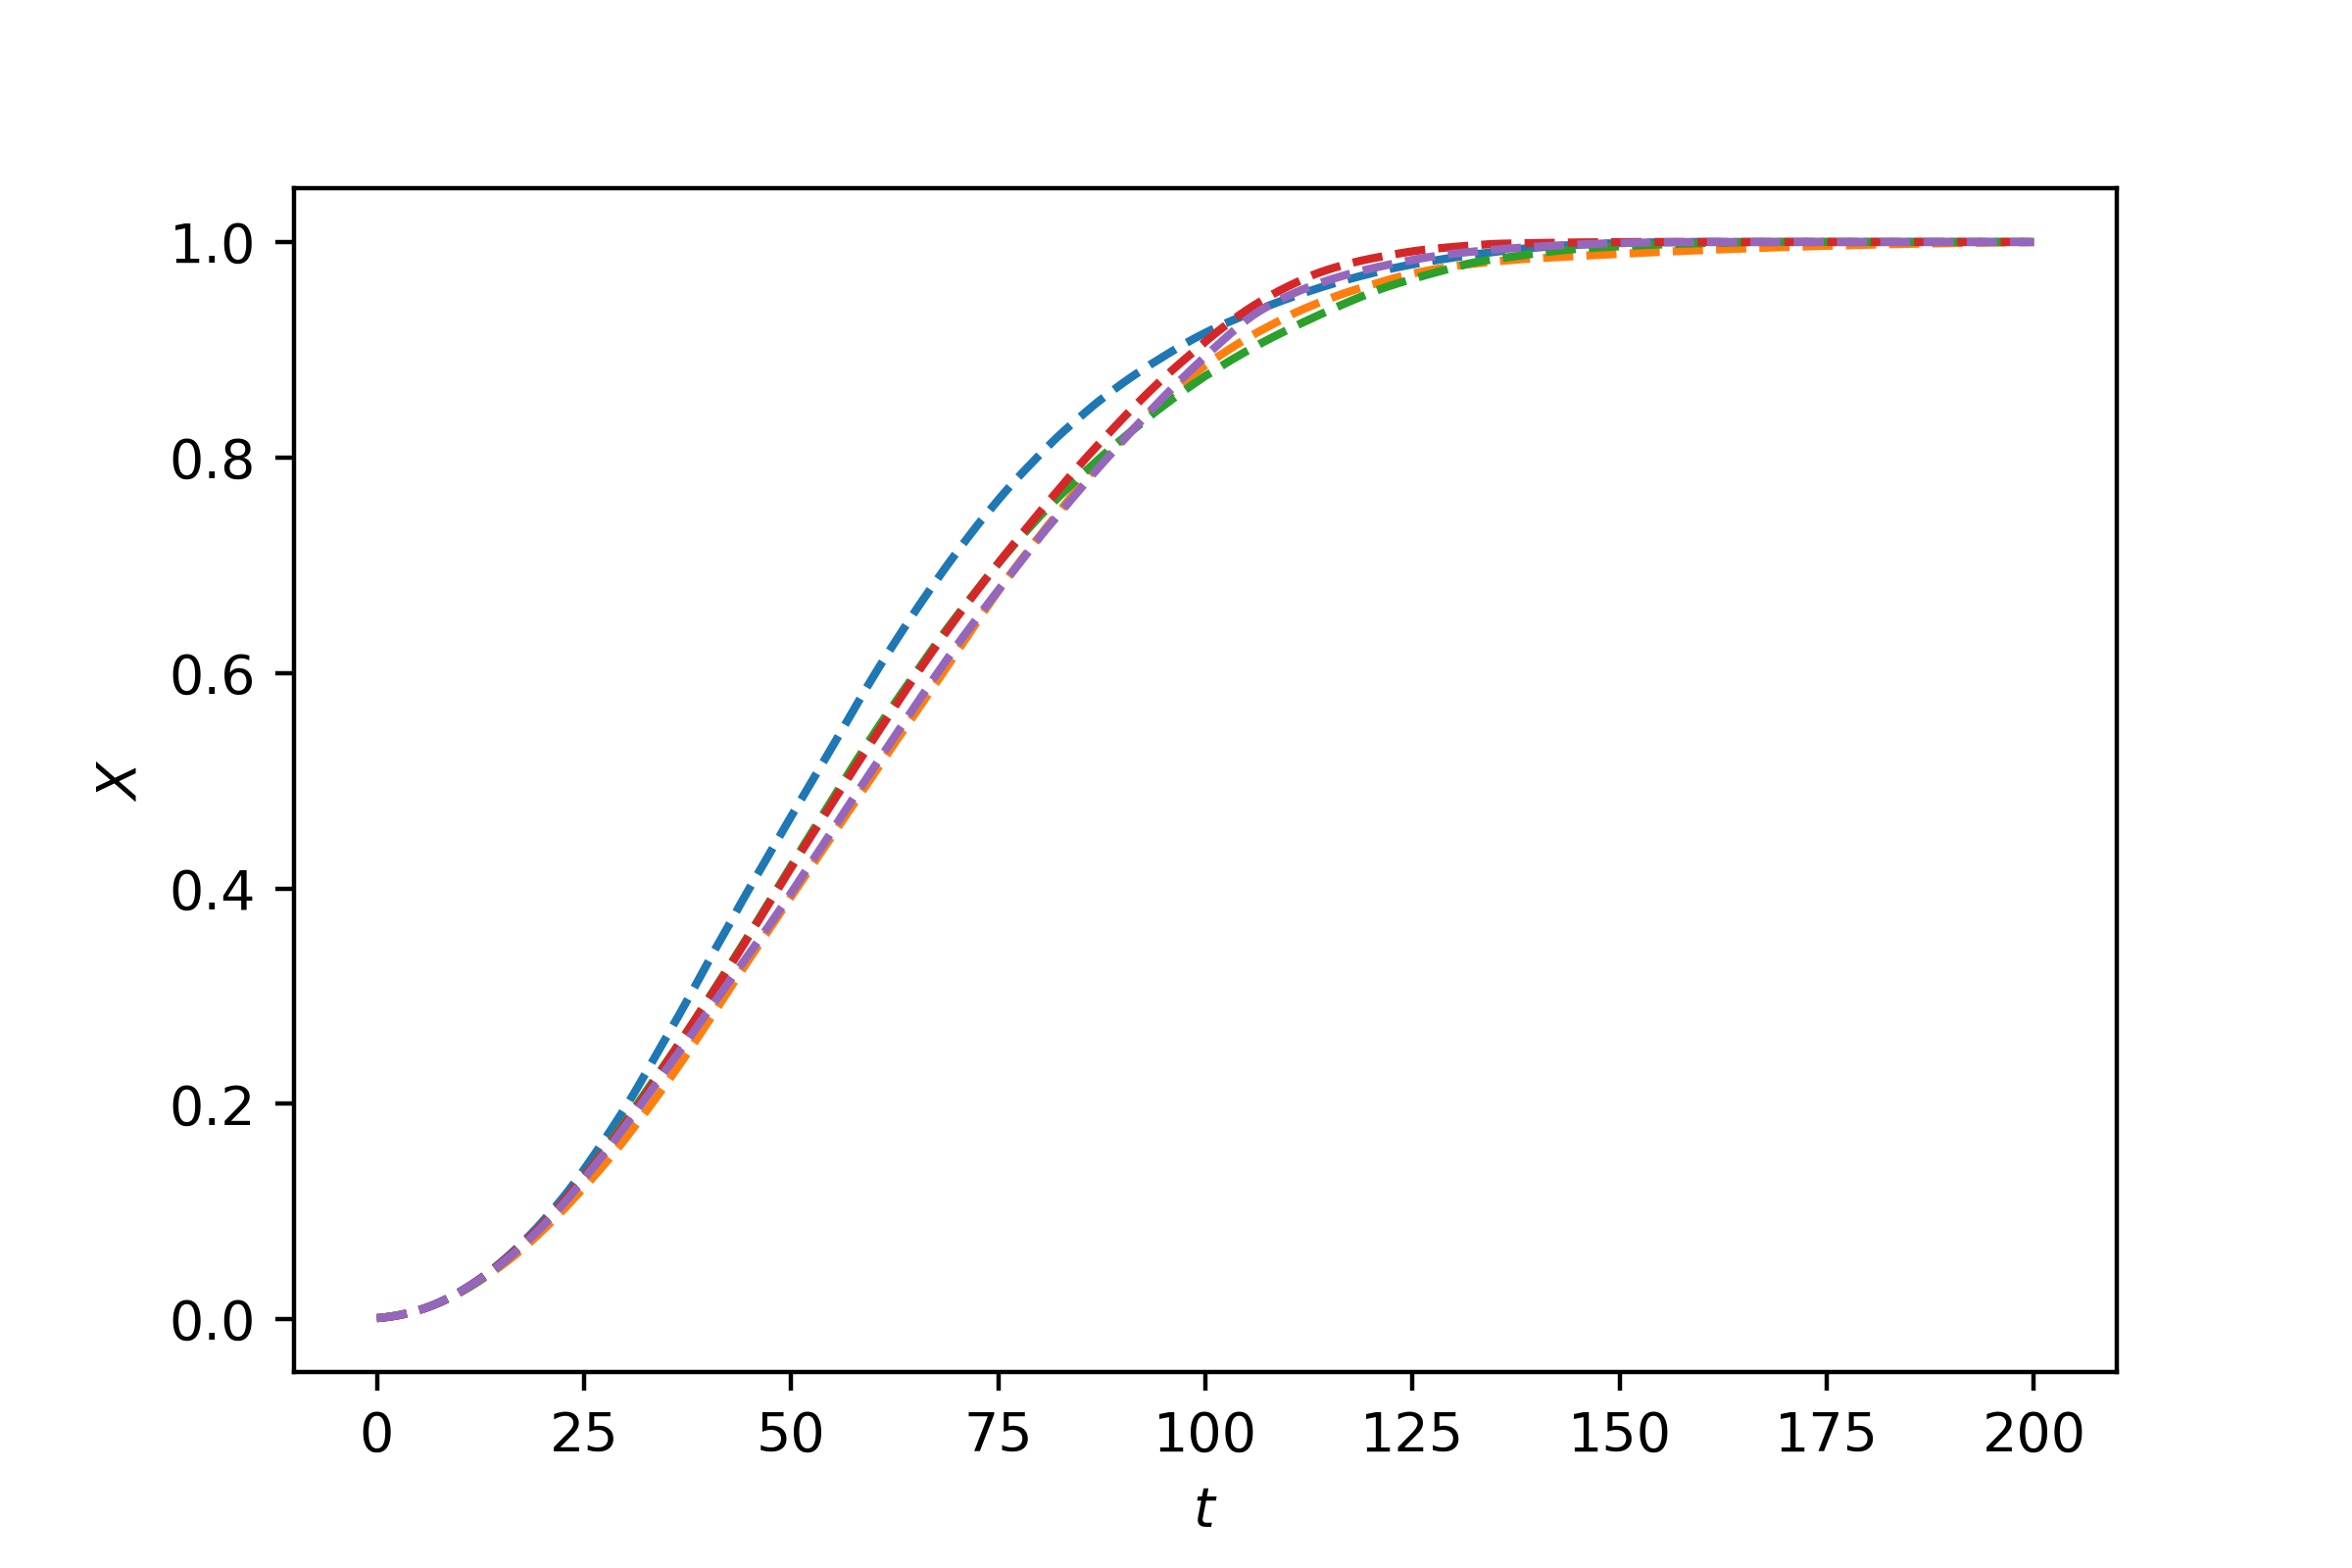
\includegraphics[scale=0.65]{solid_fraction_multiple_seed_t0.PNG}
\par\end{centering}
\caption{The solid fraction of the multiple seed homogeneous nucleation at $t=0$.}  \label{fig:solid_fraction_multiple_seed_t0}
\end{figure}
\par\end{center}
%
\begin{center}
\begin{figure} 
\begin{centering}
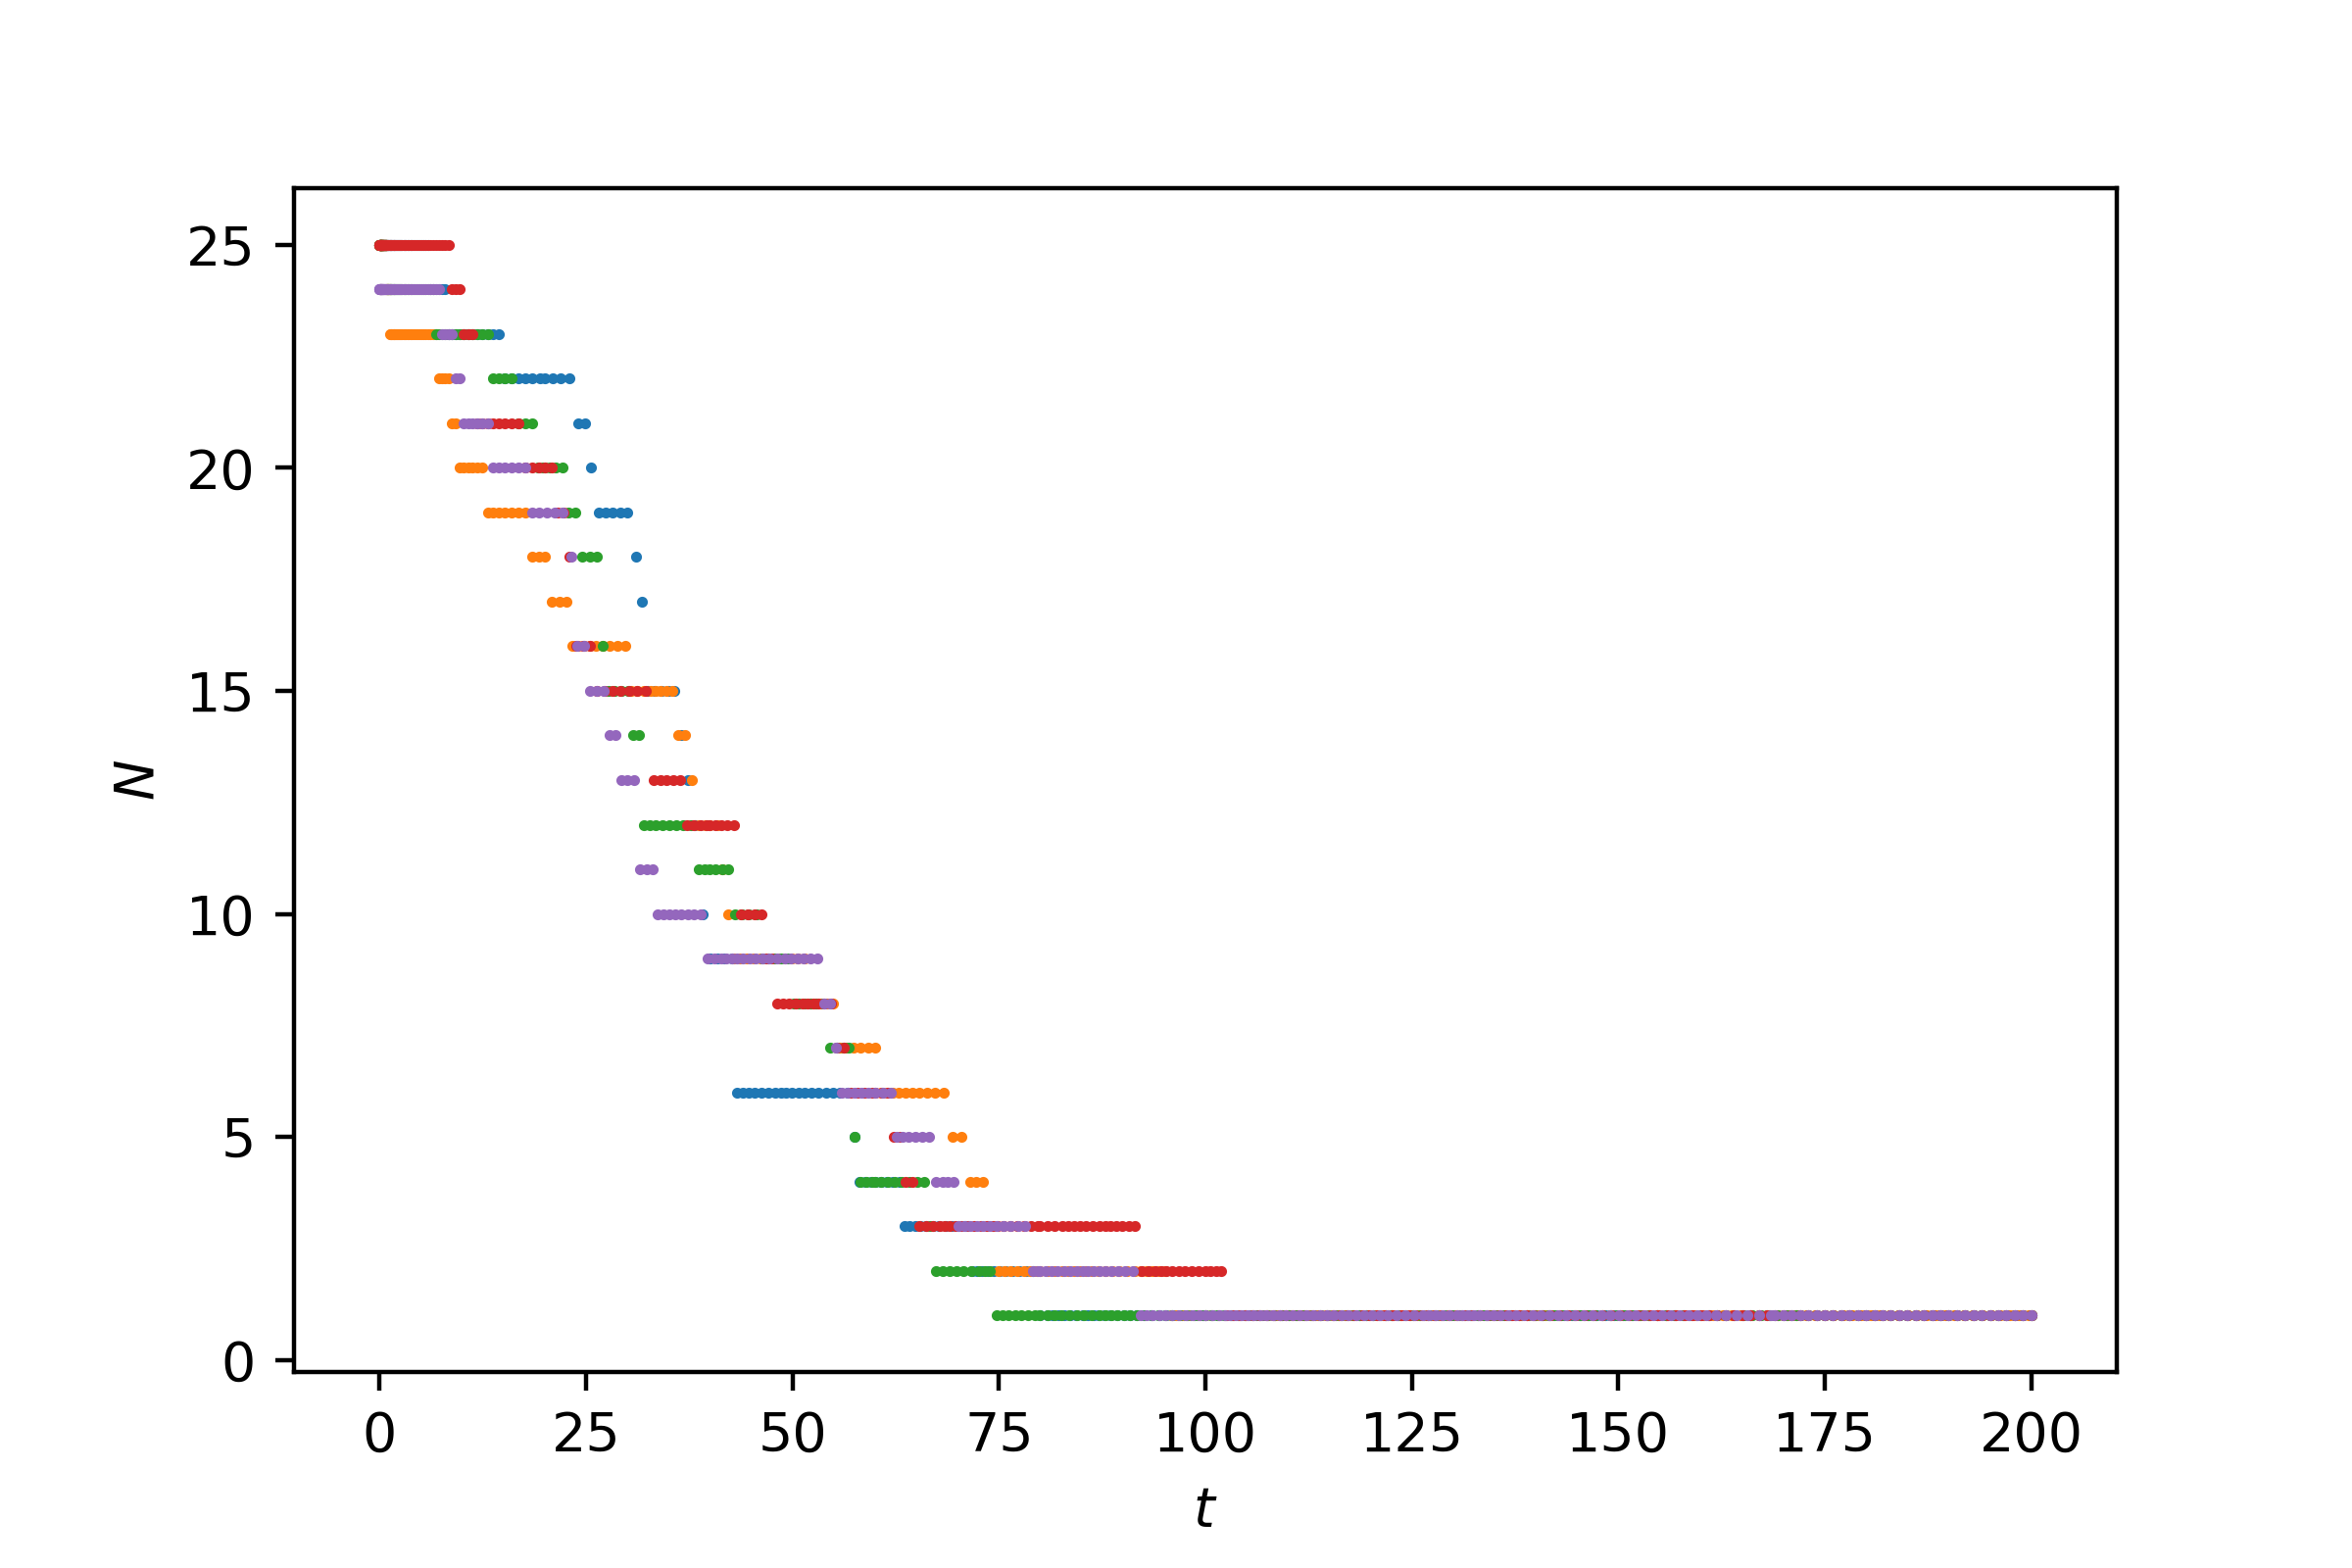
\includegraphics[scale=0.65]{particle_count_multiple_seed_t0.PNG}
\par\end{centering}
\caption{The number of discrete particles of the multiple seed homogeneous nucleation at $t=0$.} \label{fig:particle_count_multiple_seed_t0}
\end{figure}
\par\end{center}
%
\begin{center}
\begin{figure} 
\begin{centering}
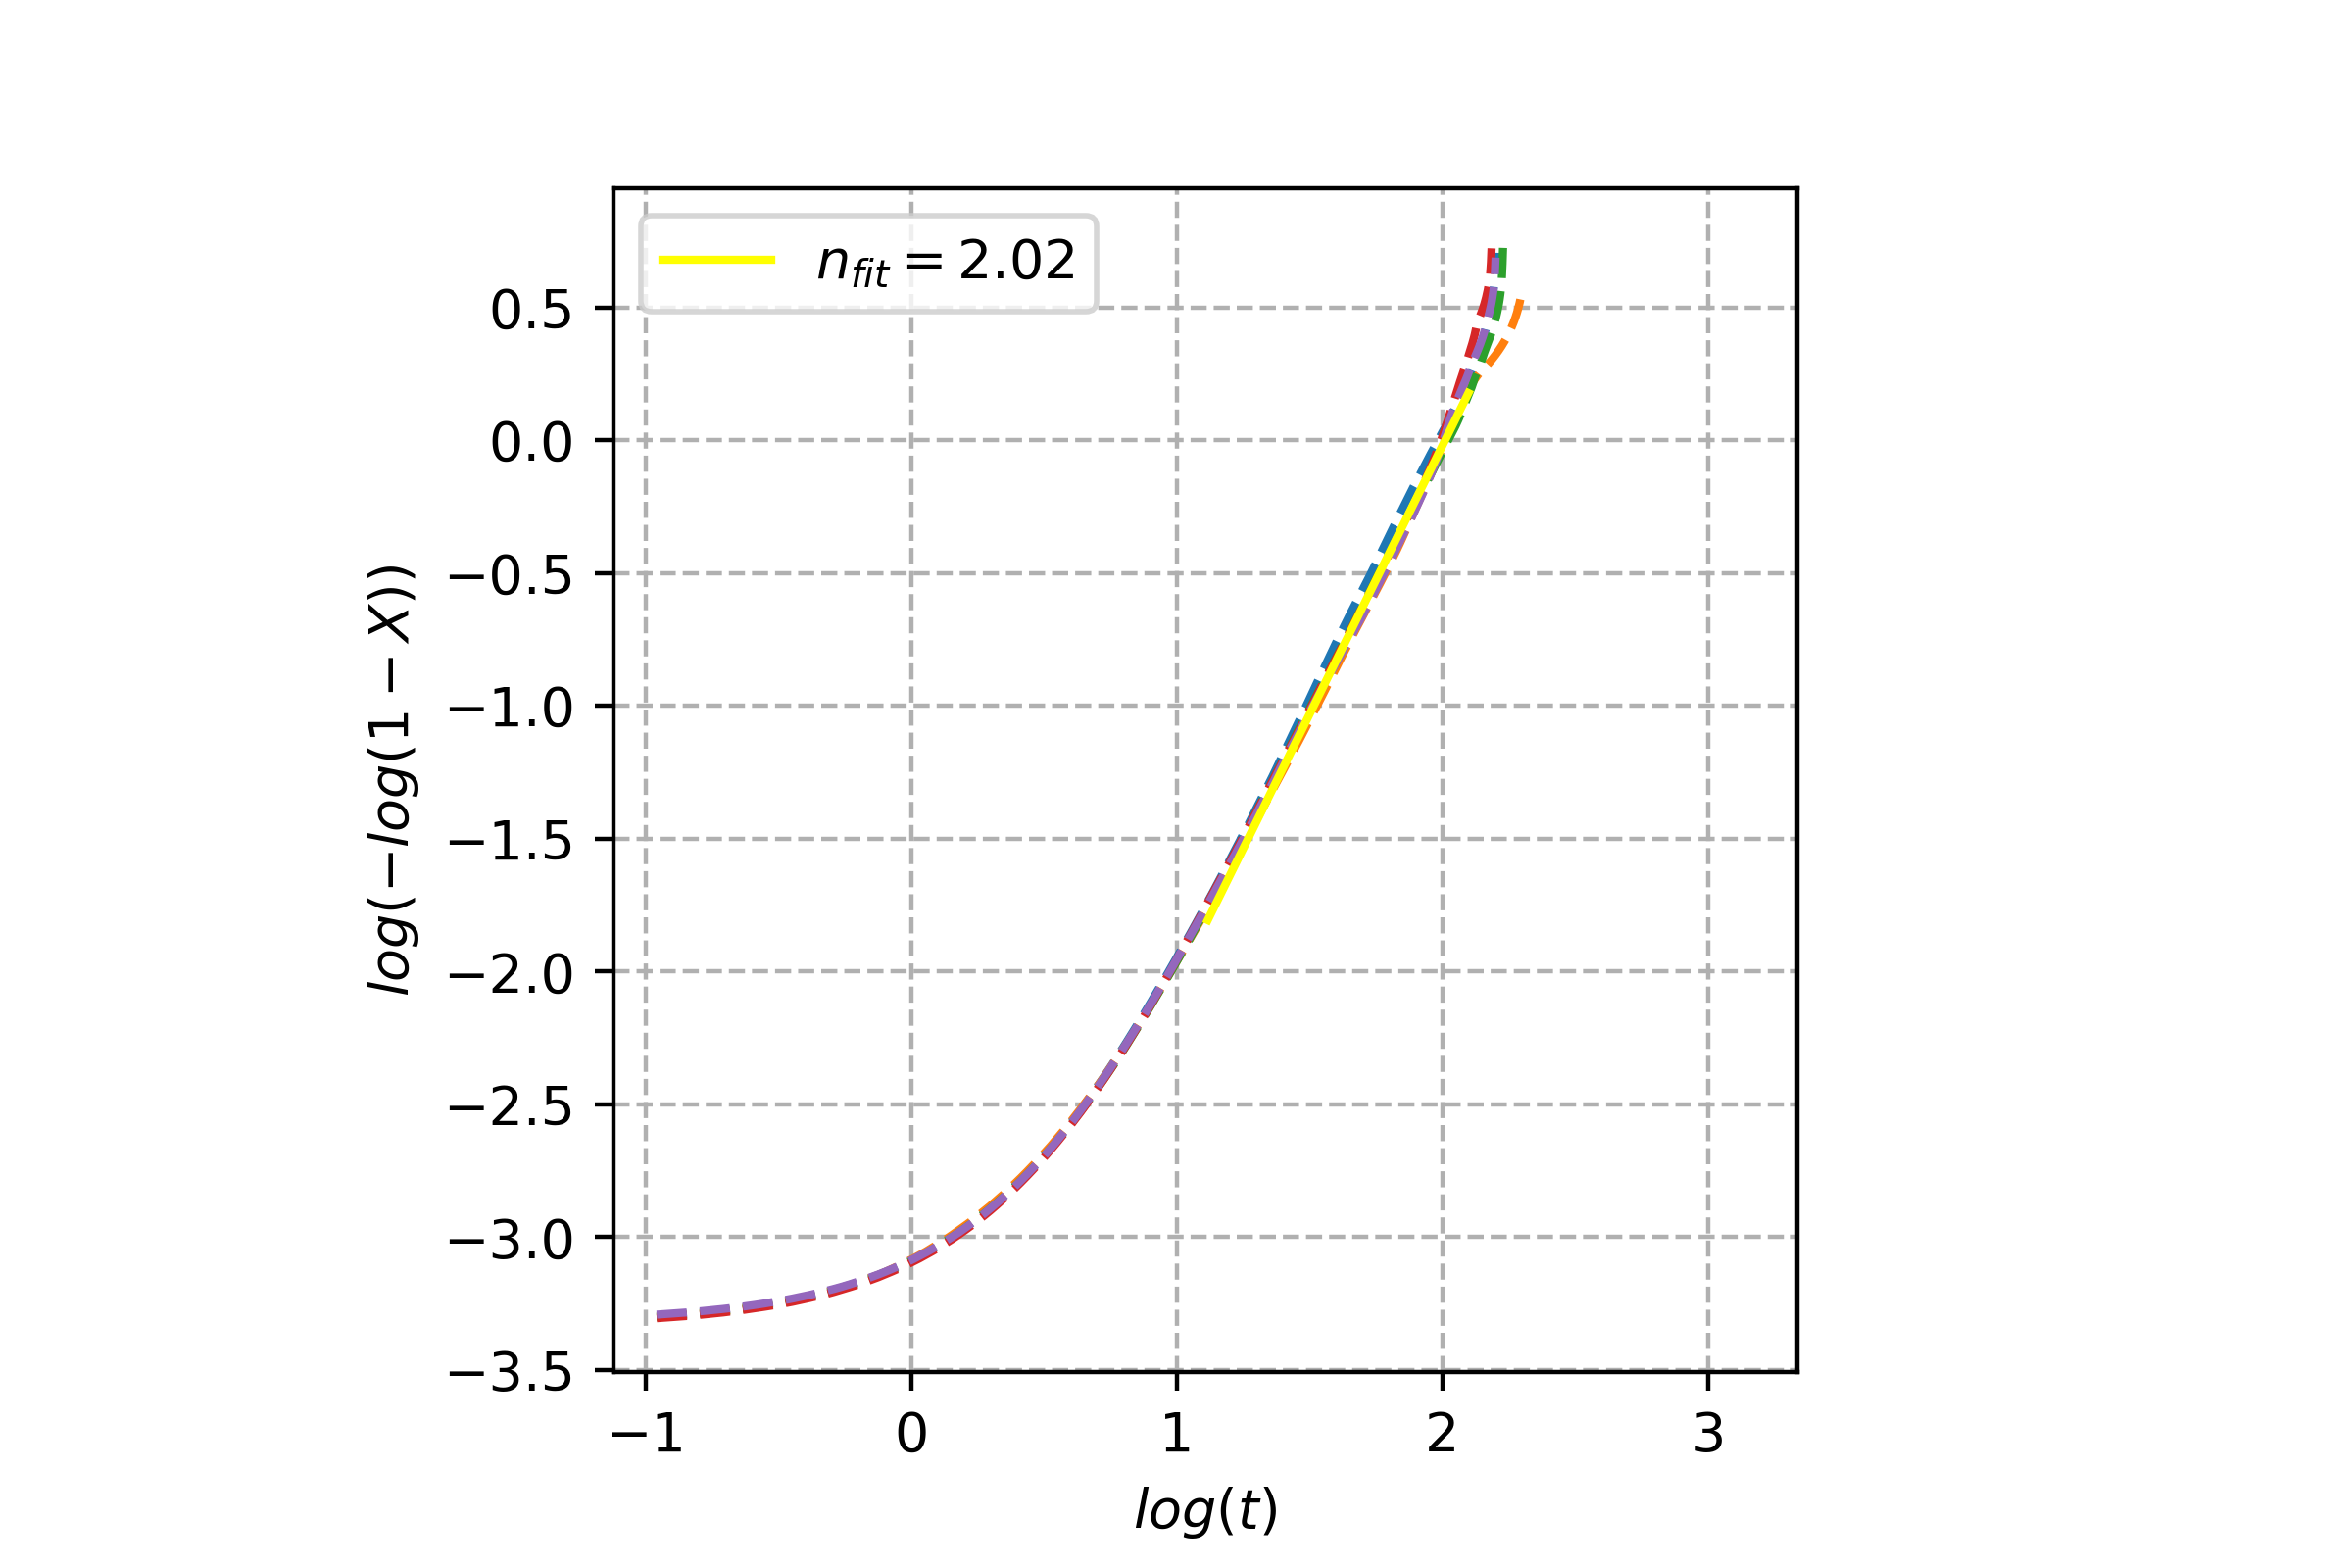
\includegraphics[scale=0.80]{Avrami_plot_multiple_seed_t0.PNG}
\par\end{centering}
\caption{The Avrami plots of the multiple seed homogeneous nucleation at $t=0$. Only one of the five fitted slopes is shown.} \label{fig:avarmi_plot_multiple_seed_t0}
\end{figure}
\par\end{center}
%
\begin{center}
\begin{figure} 
\begin{centering}
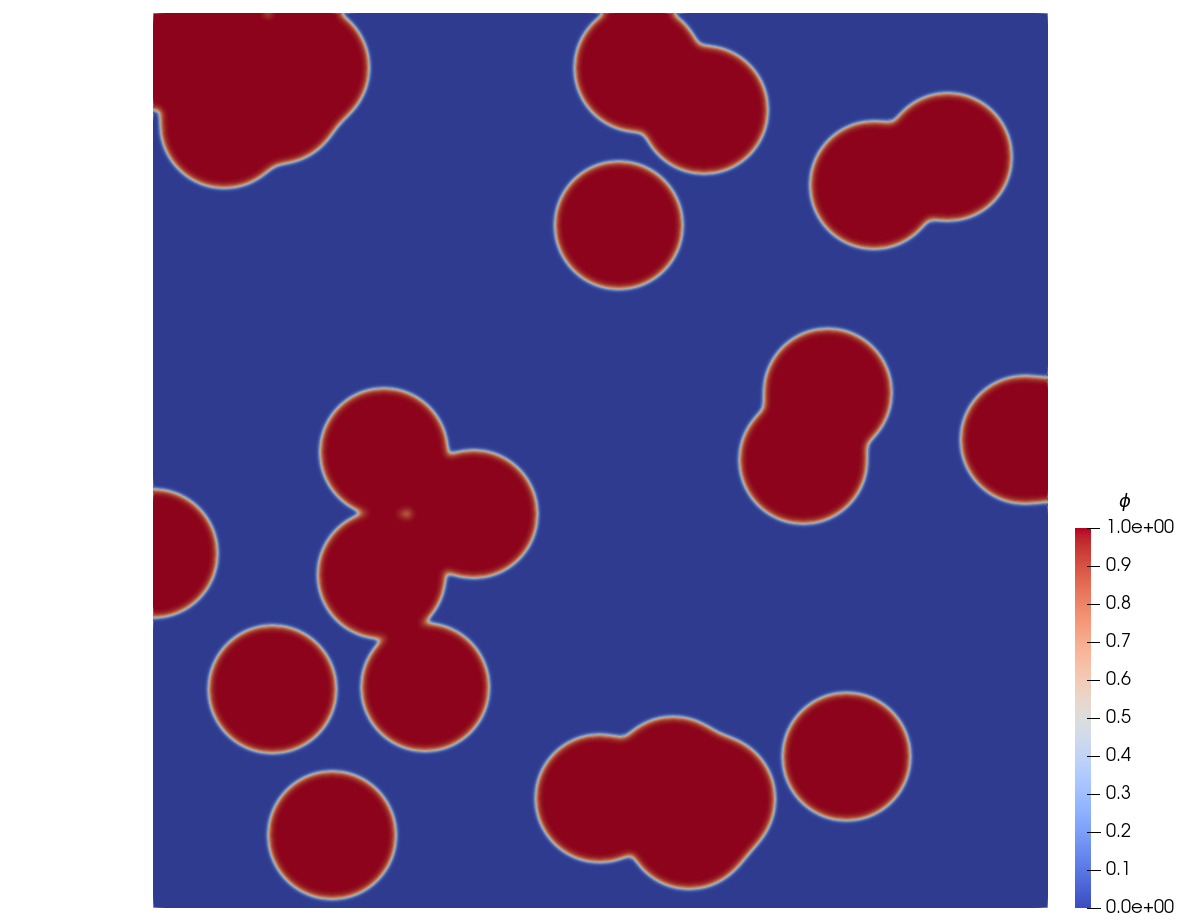
\includegraphics[scale=0.80]{t40_multiple_seed_t0.PNG}
\par\end{centering}
\caption{Snapshot of the phase-field domain at $t=40$.} \label{fig:t40_multiple_seed_t0}
\end{figure}
\par\end{center}

%COMMENT, is there a need to at least discuss the random number generator?  It's going to cause a world of hurt in reproducing this.  We should at least acknowledge this even if we don't have a solution
\subsection{Explicit nucleation, multiple seeds at random times}

For this part of the homogeneous nucleation benchmark problem we examine the nucleation behavior when multiple seeds are inserted at random times. We use the same metrics as in the previous problem,  (Fig.~\ref{fig:free_energy_multiple_seed_randt}, ~\ref{fig:solid_fraction_multiple_seed_randt}, ~\ref{fig:particle_count_multiple_seed_randt},~\ref{fig:avarmi_plot_multiple_seed_randt}) with also a snapshot of the phase-field domain at $t=100$ as shown in Fig.~\ref{fig:t100_multiple_seed_randt}. %{\bf Olle: Need to have snapshot in the problem specification}

Similar to what we observed for homogeneous nucleation with multiple seeds at the same time, the total free energy decreases monotonically as shown in Fig.~\ref{fig:free_energy_multiple_seed_randt}, and the solid fraction increases monotonically. The main difference %compared to the previous problem 
is related to the shape change of the solid-fraction curve. Transformations are observed to follow a characteristic S-shaped, or sigmoidal profile (as shown in  Fig.~\ref{fig:solid_fraction_multiple_seed_randt}), where the transformation rates are low at the beginning and the end of the transformation but rapid in between. (In contrast, for homogeneous nucleation with multiple seeds at $t=0$, the Avrami plots are approximately straight lines after the initial slow growth, Fig. \ref{fig:avarmi_plot_multiple_seed_t0}.) The initial slow rate can be attributed to the time required for forming a significant number of nuclei of the solid phase. During the intermediate period the transformation is rapid as the nuclei grow into particles and consume the old liquid phase while nuclei continue to form in the remaining liquid phase. Once the transformation begins to near completion the liquid phase in the domain has almost all been consumed: there is not much space left for nuclei to form and the production of new particles slows down. Furthermore, the particles already existing begin to overlap, forming a boundary where growth of solid phase stops. Figure~\ref{fig:t100_multiple_seed_randt} is an example showing the growth of the particles at $t=100$. Notice that in contrast with the snapshot shown in Fig.~\ref{fig:t100_multiple_seed_randt}, this time the particles have different sizes since the seeds are inserted at different times. %{\bf Need to specify that snapshot needs to be generated and at what time - I think it maybe better if snapshots are both at the same time.} 
The number of discrete particles is 0 at $t=0$. As the time increases up to around $t=200$, more new nuclei are added to the system at at rate that outpaces nuclei merging events, resulting in an overall increase in the number of discrete particles. After that, the merging rate is greater than the insertion rate. Therefore, the number of discrete particles starts to decrease and finally drops to unity as in the homogeneous nucleation with seeds at $t=0$. For a quantitative comparison of the nucleation kinetics, we calculate the slope of the Avrami plots. This time when nucleation happens at different random times, and the slope of the Avrami plots should be around 3.0, according the JMAK theory (two dimensions of growth plus one, a constant growth rate). We fit a straight line to the data ranging from $1.5 < \log t < 2.5$. The average slope of the fitted line for the five runs is $n=3.07$, and the variance is $0.03$.  Although the Avrami plots of the five runs with different initial random positions do not overlap as well as for the case with all seeds at $t=0$, the average slope is close to the expected value 3.0 and the variance is small.  This again indicates that the nucleation kinetics do not depend on the choice of the RNG seed. 

%
\begin{center}
\begin{figure} 
\begin{centering}
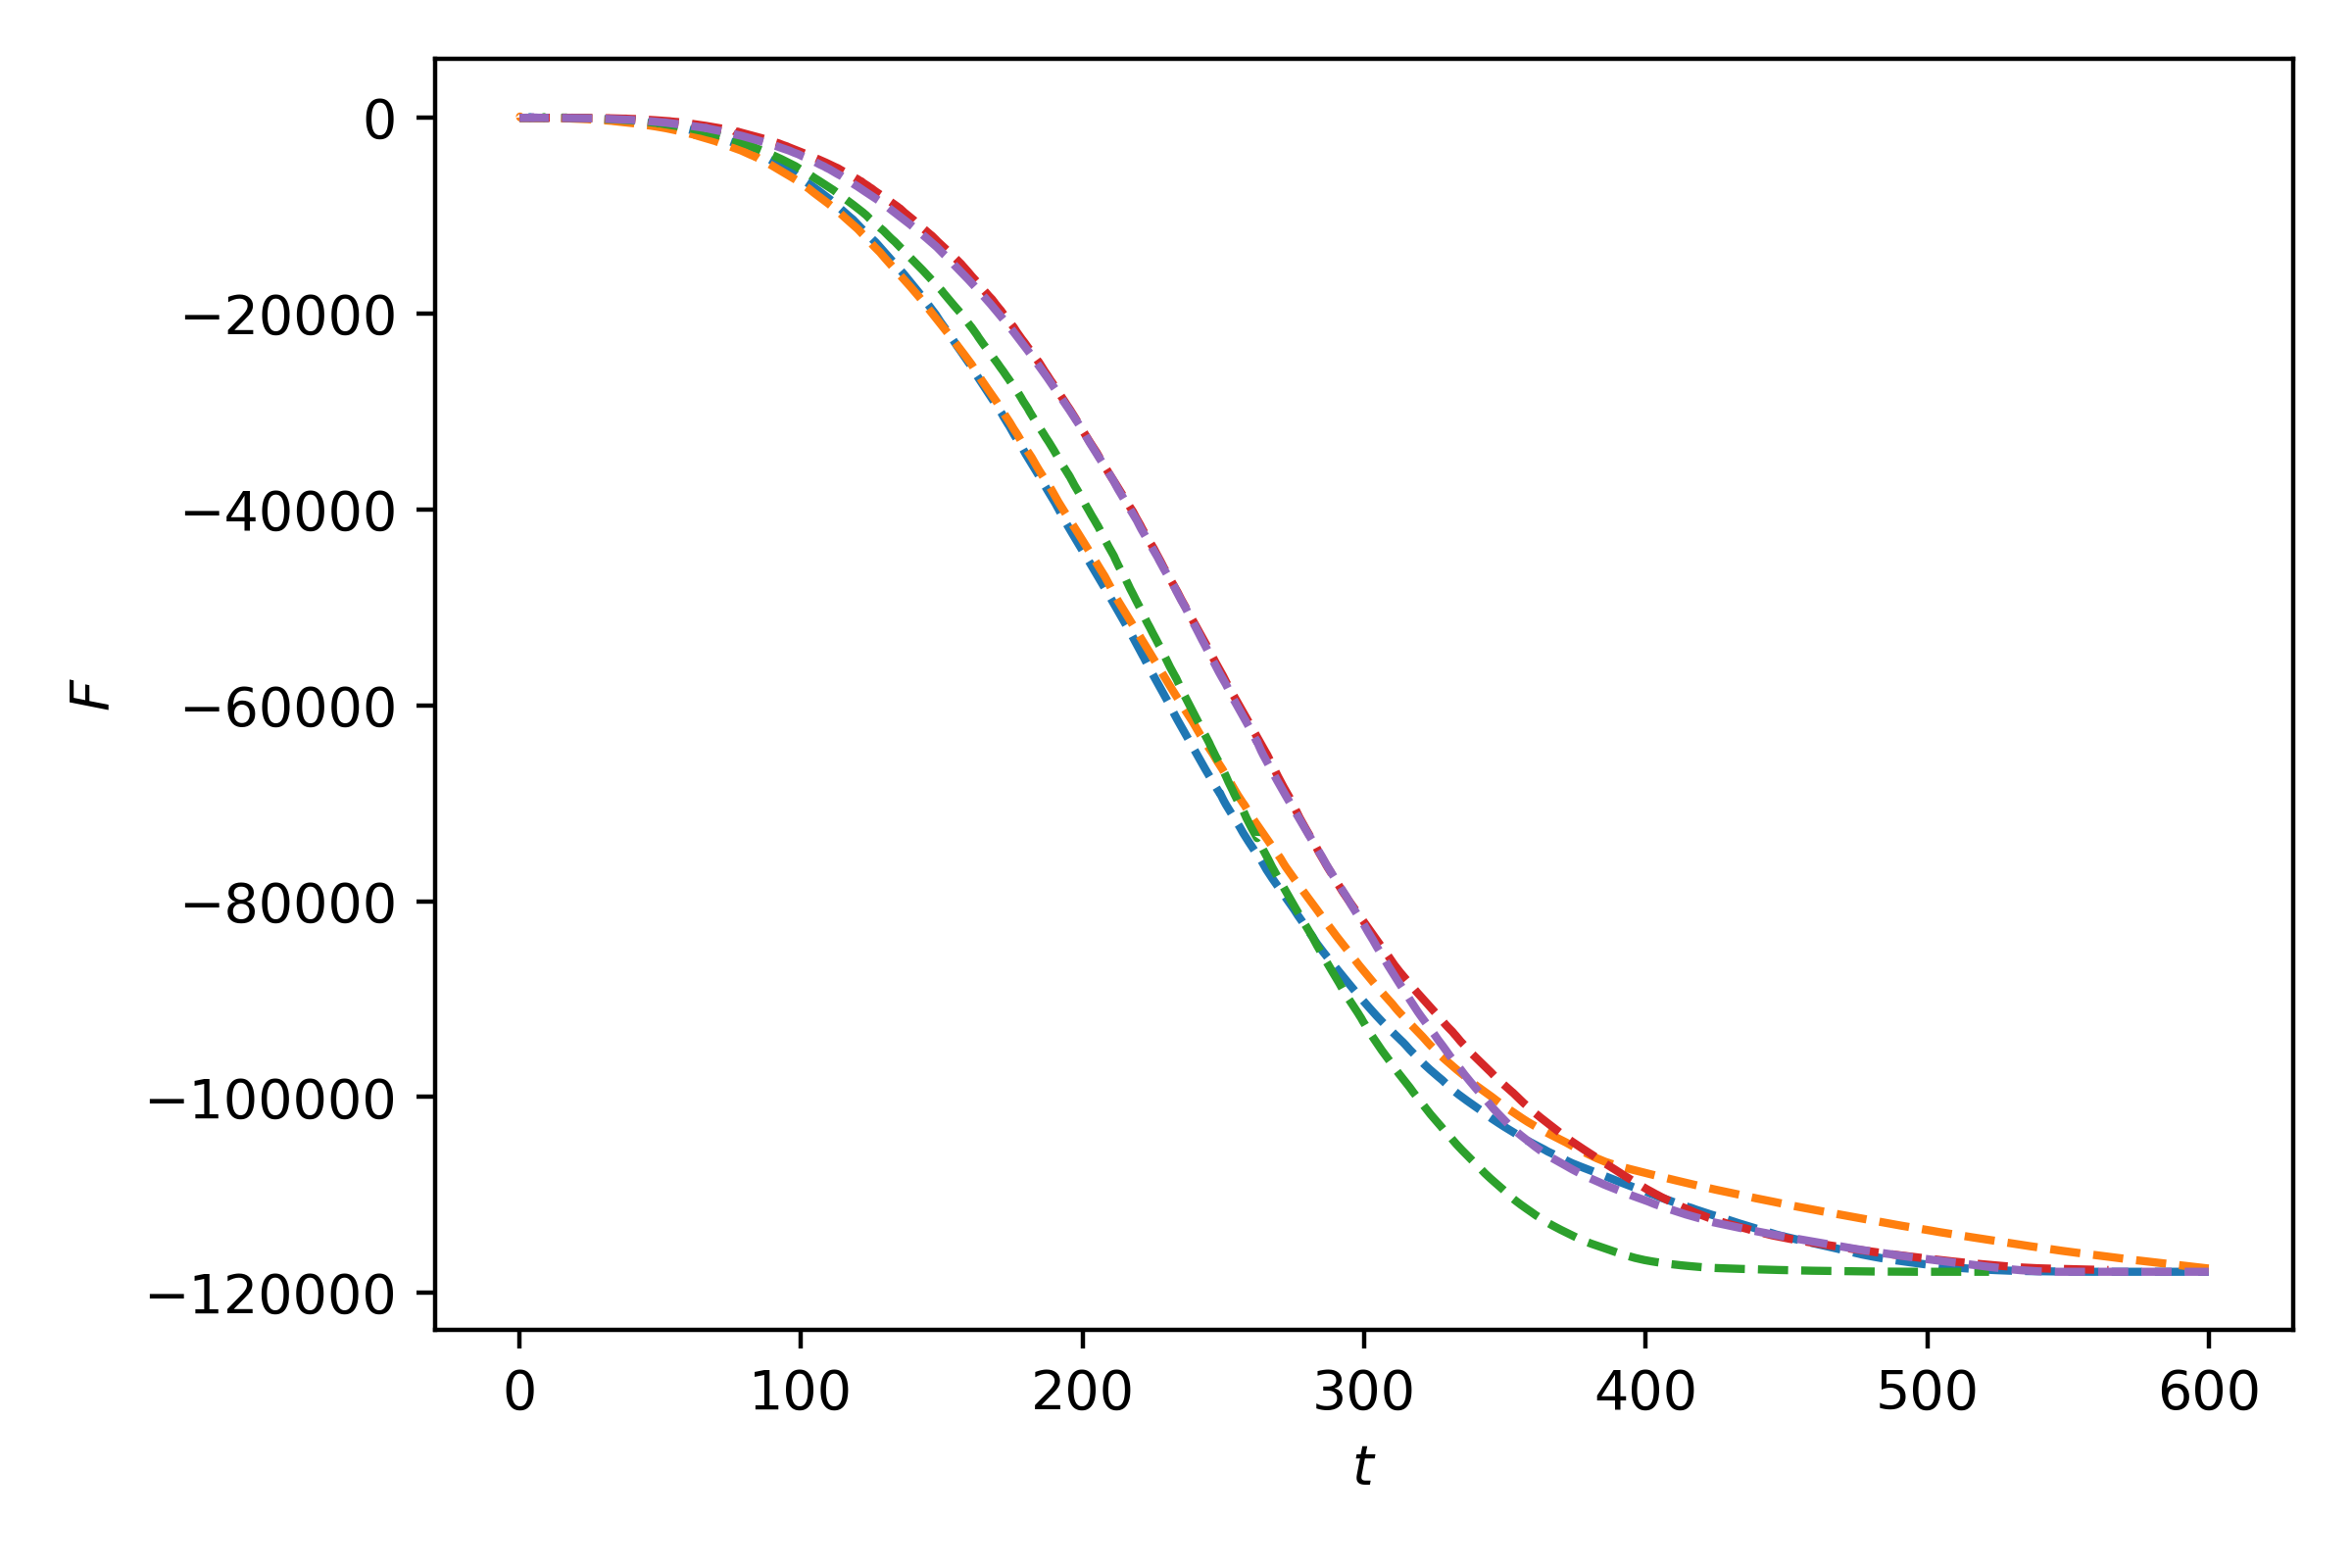
\includegraphics[scale=0.65]{free_energy_multiple_seed_randt.PNG}
\par\end{centering}
\caption{The total free energy evolution of the multiple seed homogeneous nucleation at random times.} \label{fig:free_energy_multiple_seed_randt}
\end{figure}
\par\end{center}
%
\begin{center}
\begin{figure} 
\begin{centering}
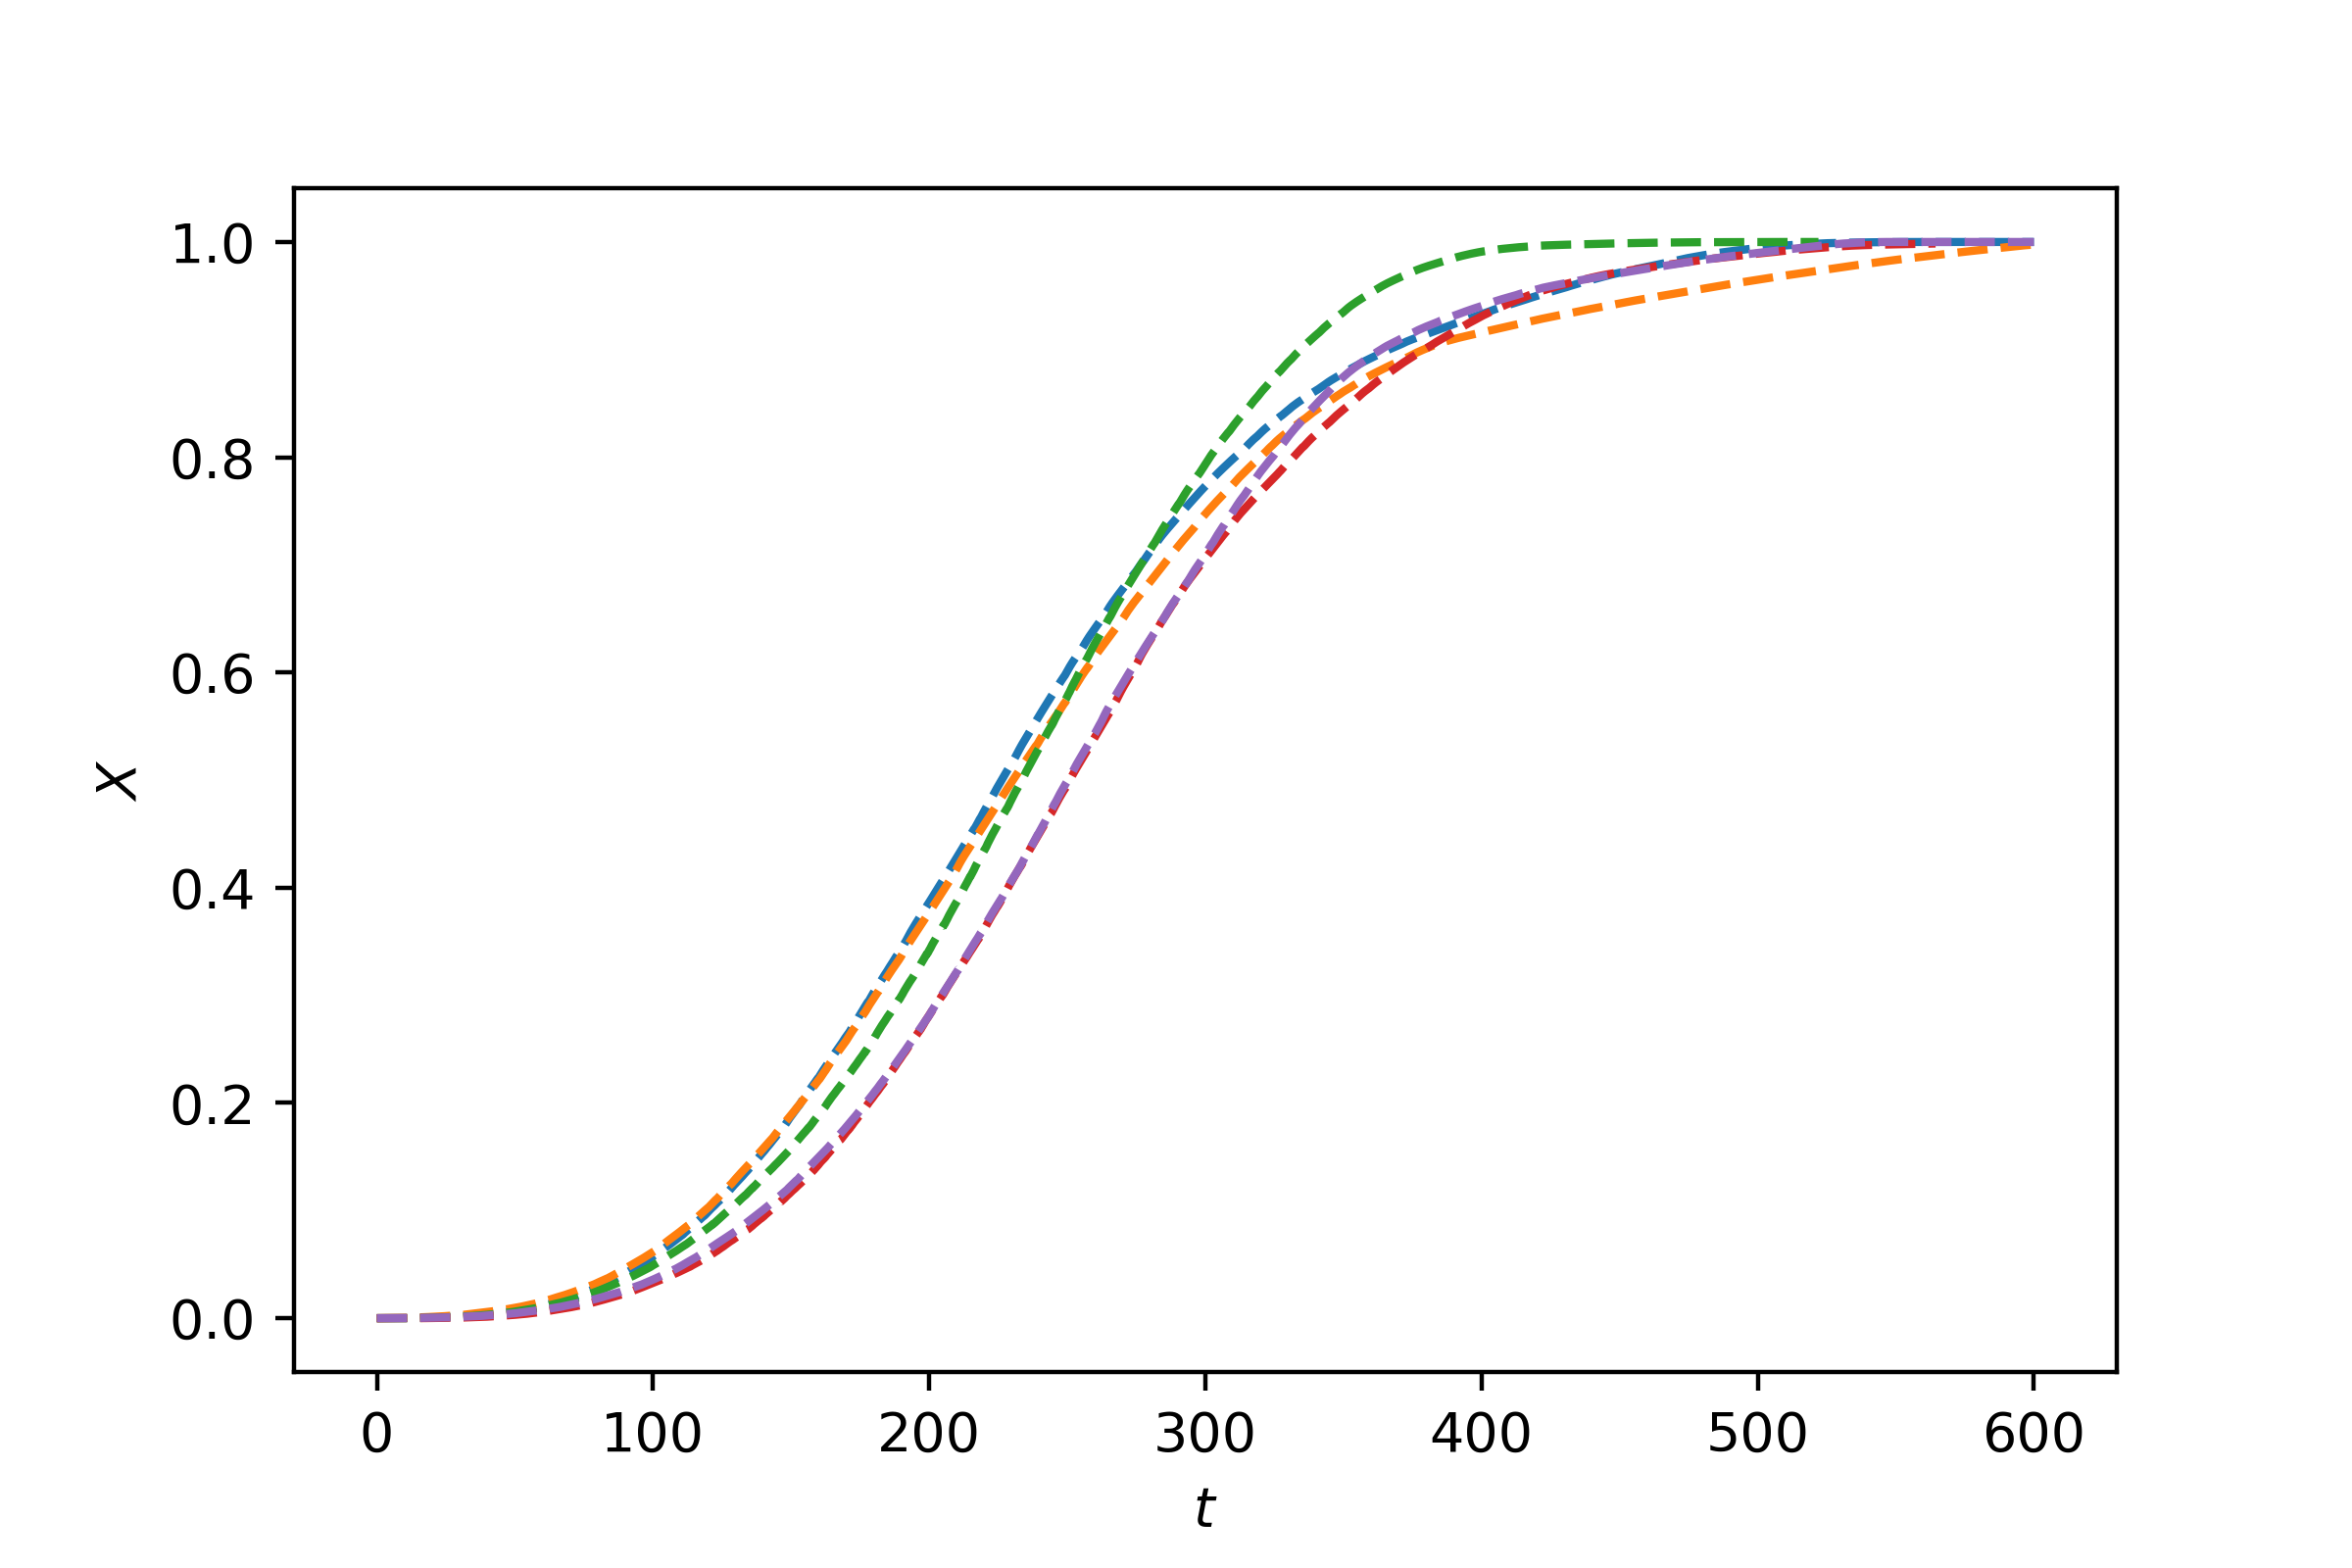
\includegraphics[scale=0.65]{solid_fraction_multiple_seed_randt.PNG}
\par\end{centering}
\caption{The solid fraction of the multiple seed homogeneous nucleation at random times.}  \label{fig:solid_fraction_multiple_seed_randt}
\end{figure}
\par\end{center}
%
\begin{center}
\begin{figure} 
\begin{centering}
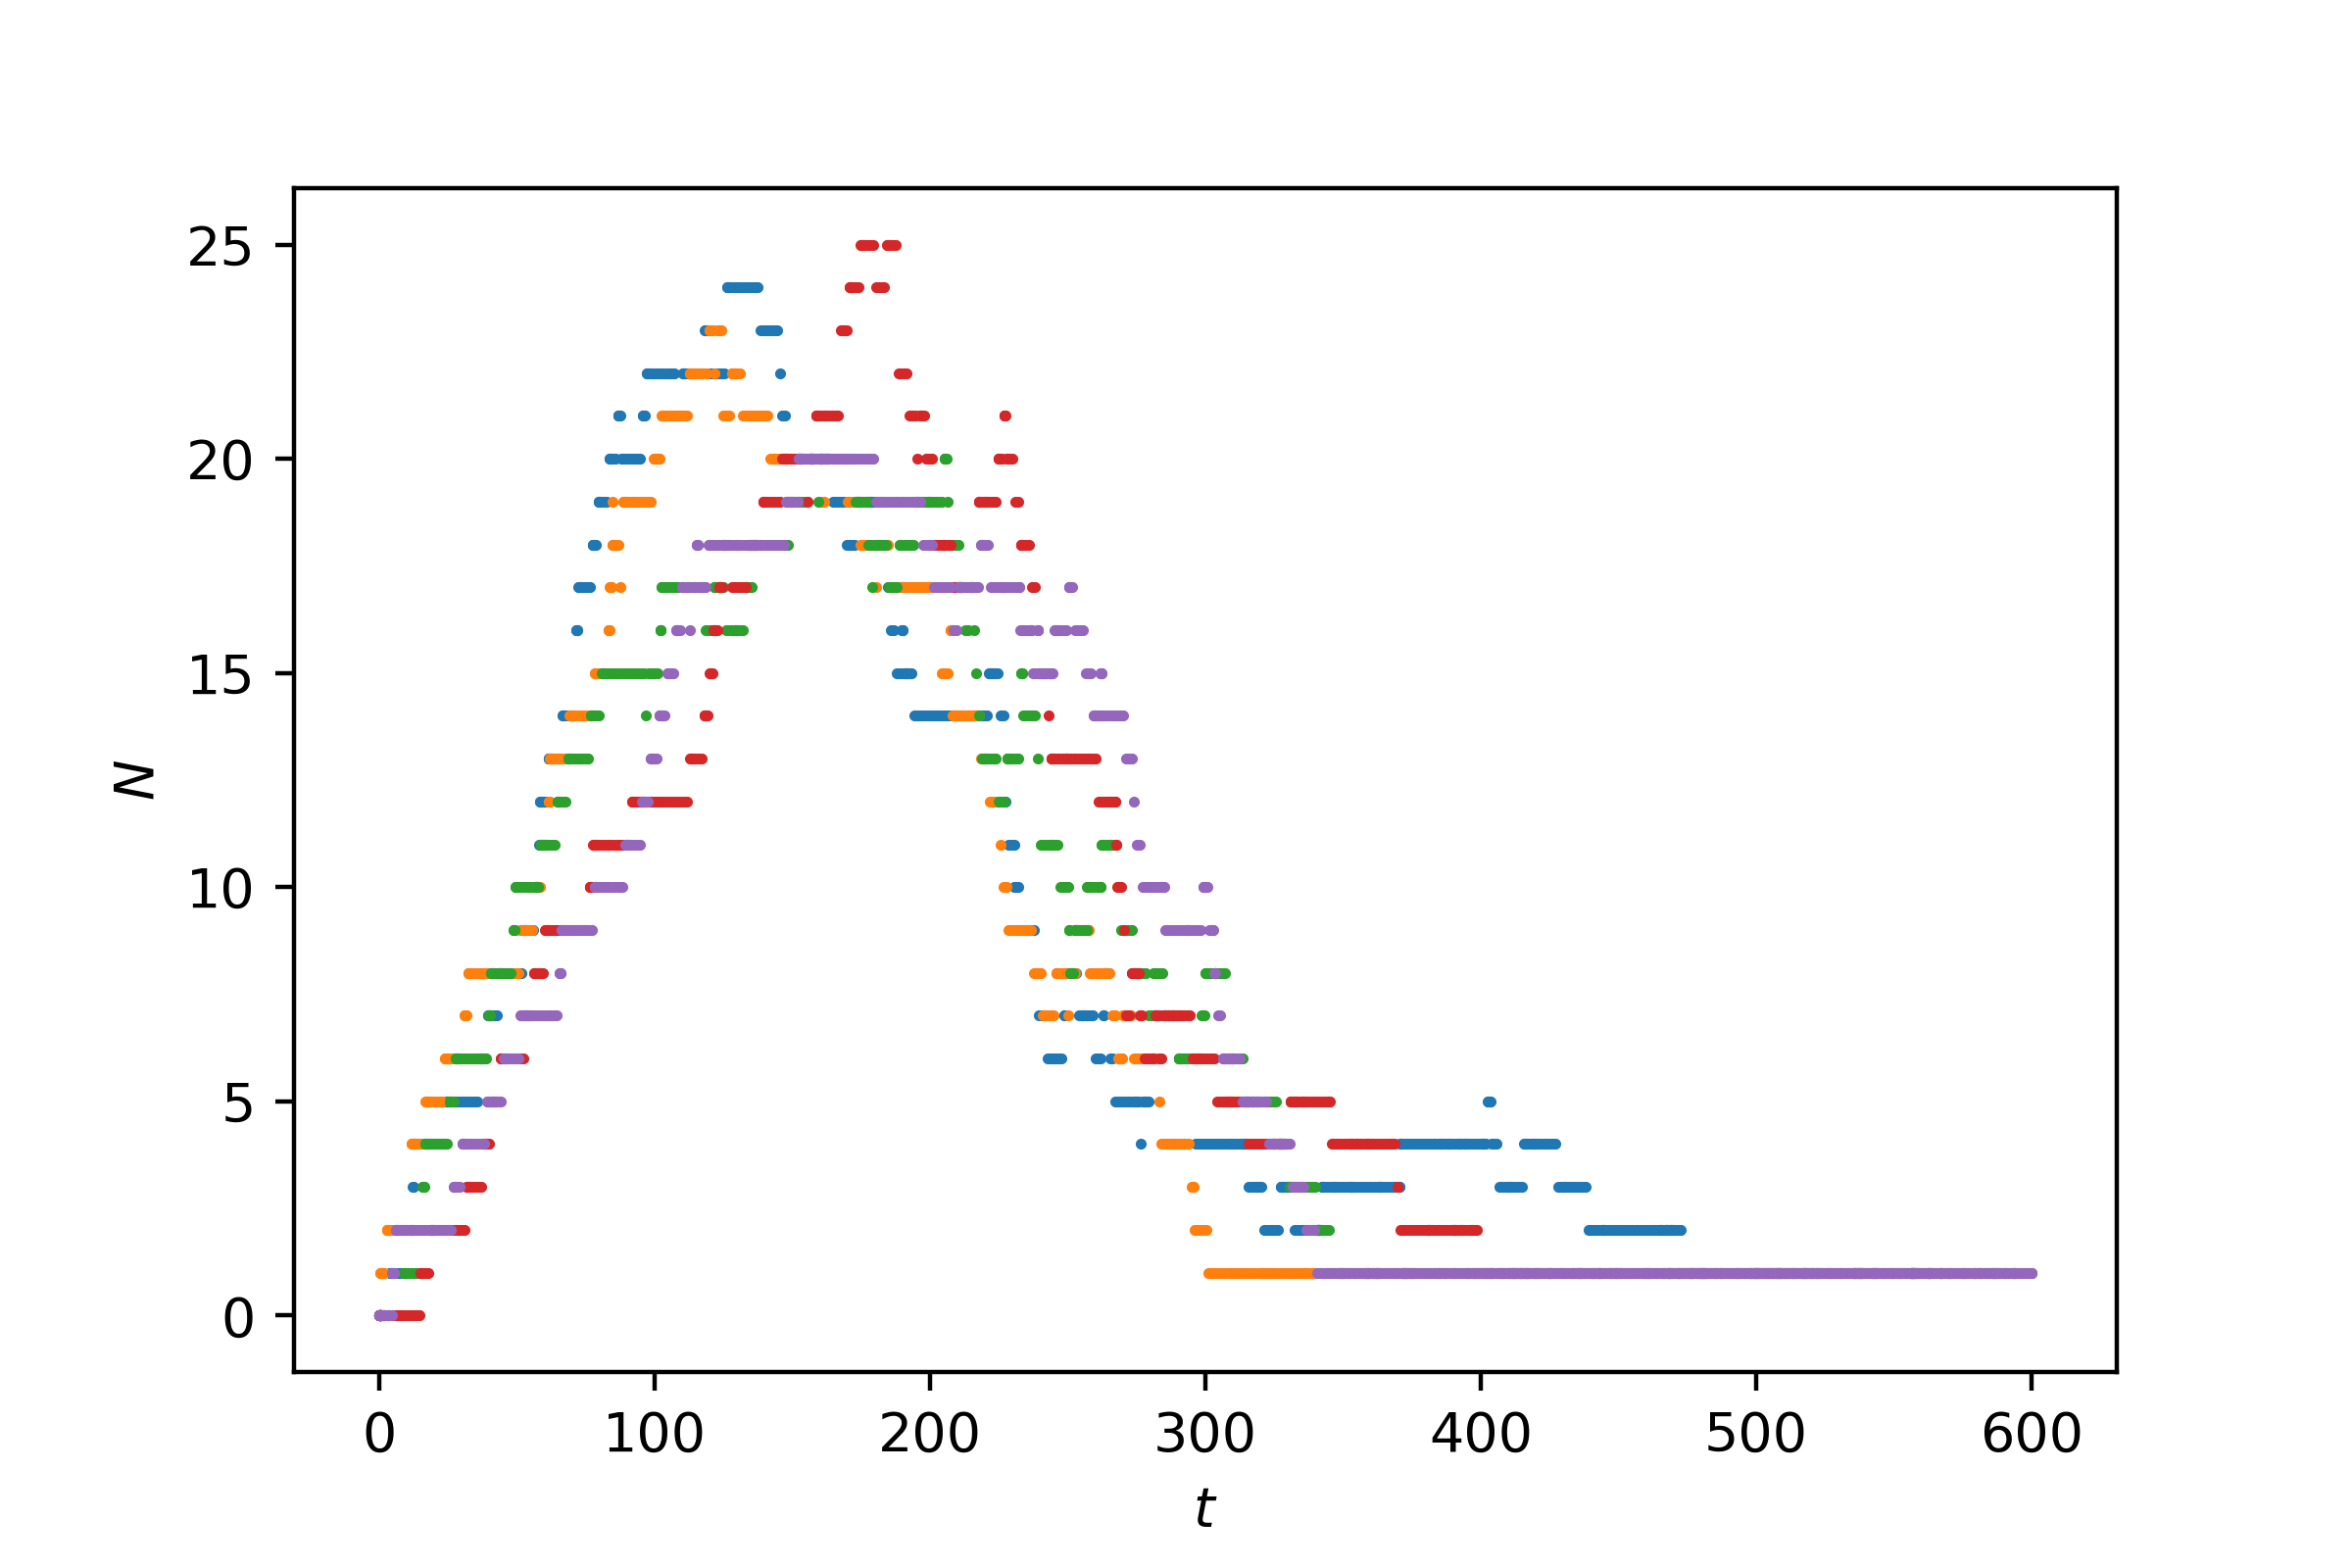
\includegraphics[scale=0.65]{particle_count_multiple_seed_randt.PNG}
\par\end{centering}
\caption{The number of discrete particles of the multiple seed homogeneous nucleation at random times.} \label{fig:particle_count_multiple_seed_randt}
\end{figure}
\par\end{center}
%
\begin{center}
\begin{figure} 
\begin{centering}
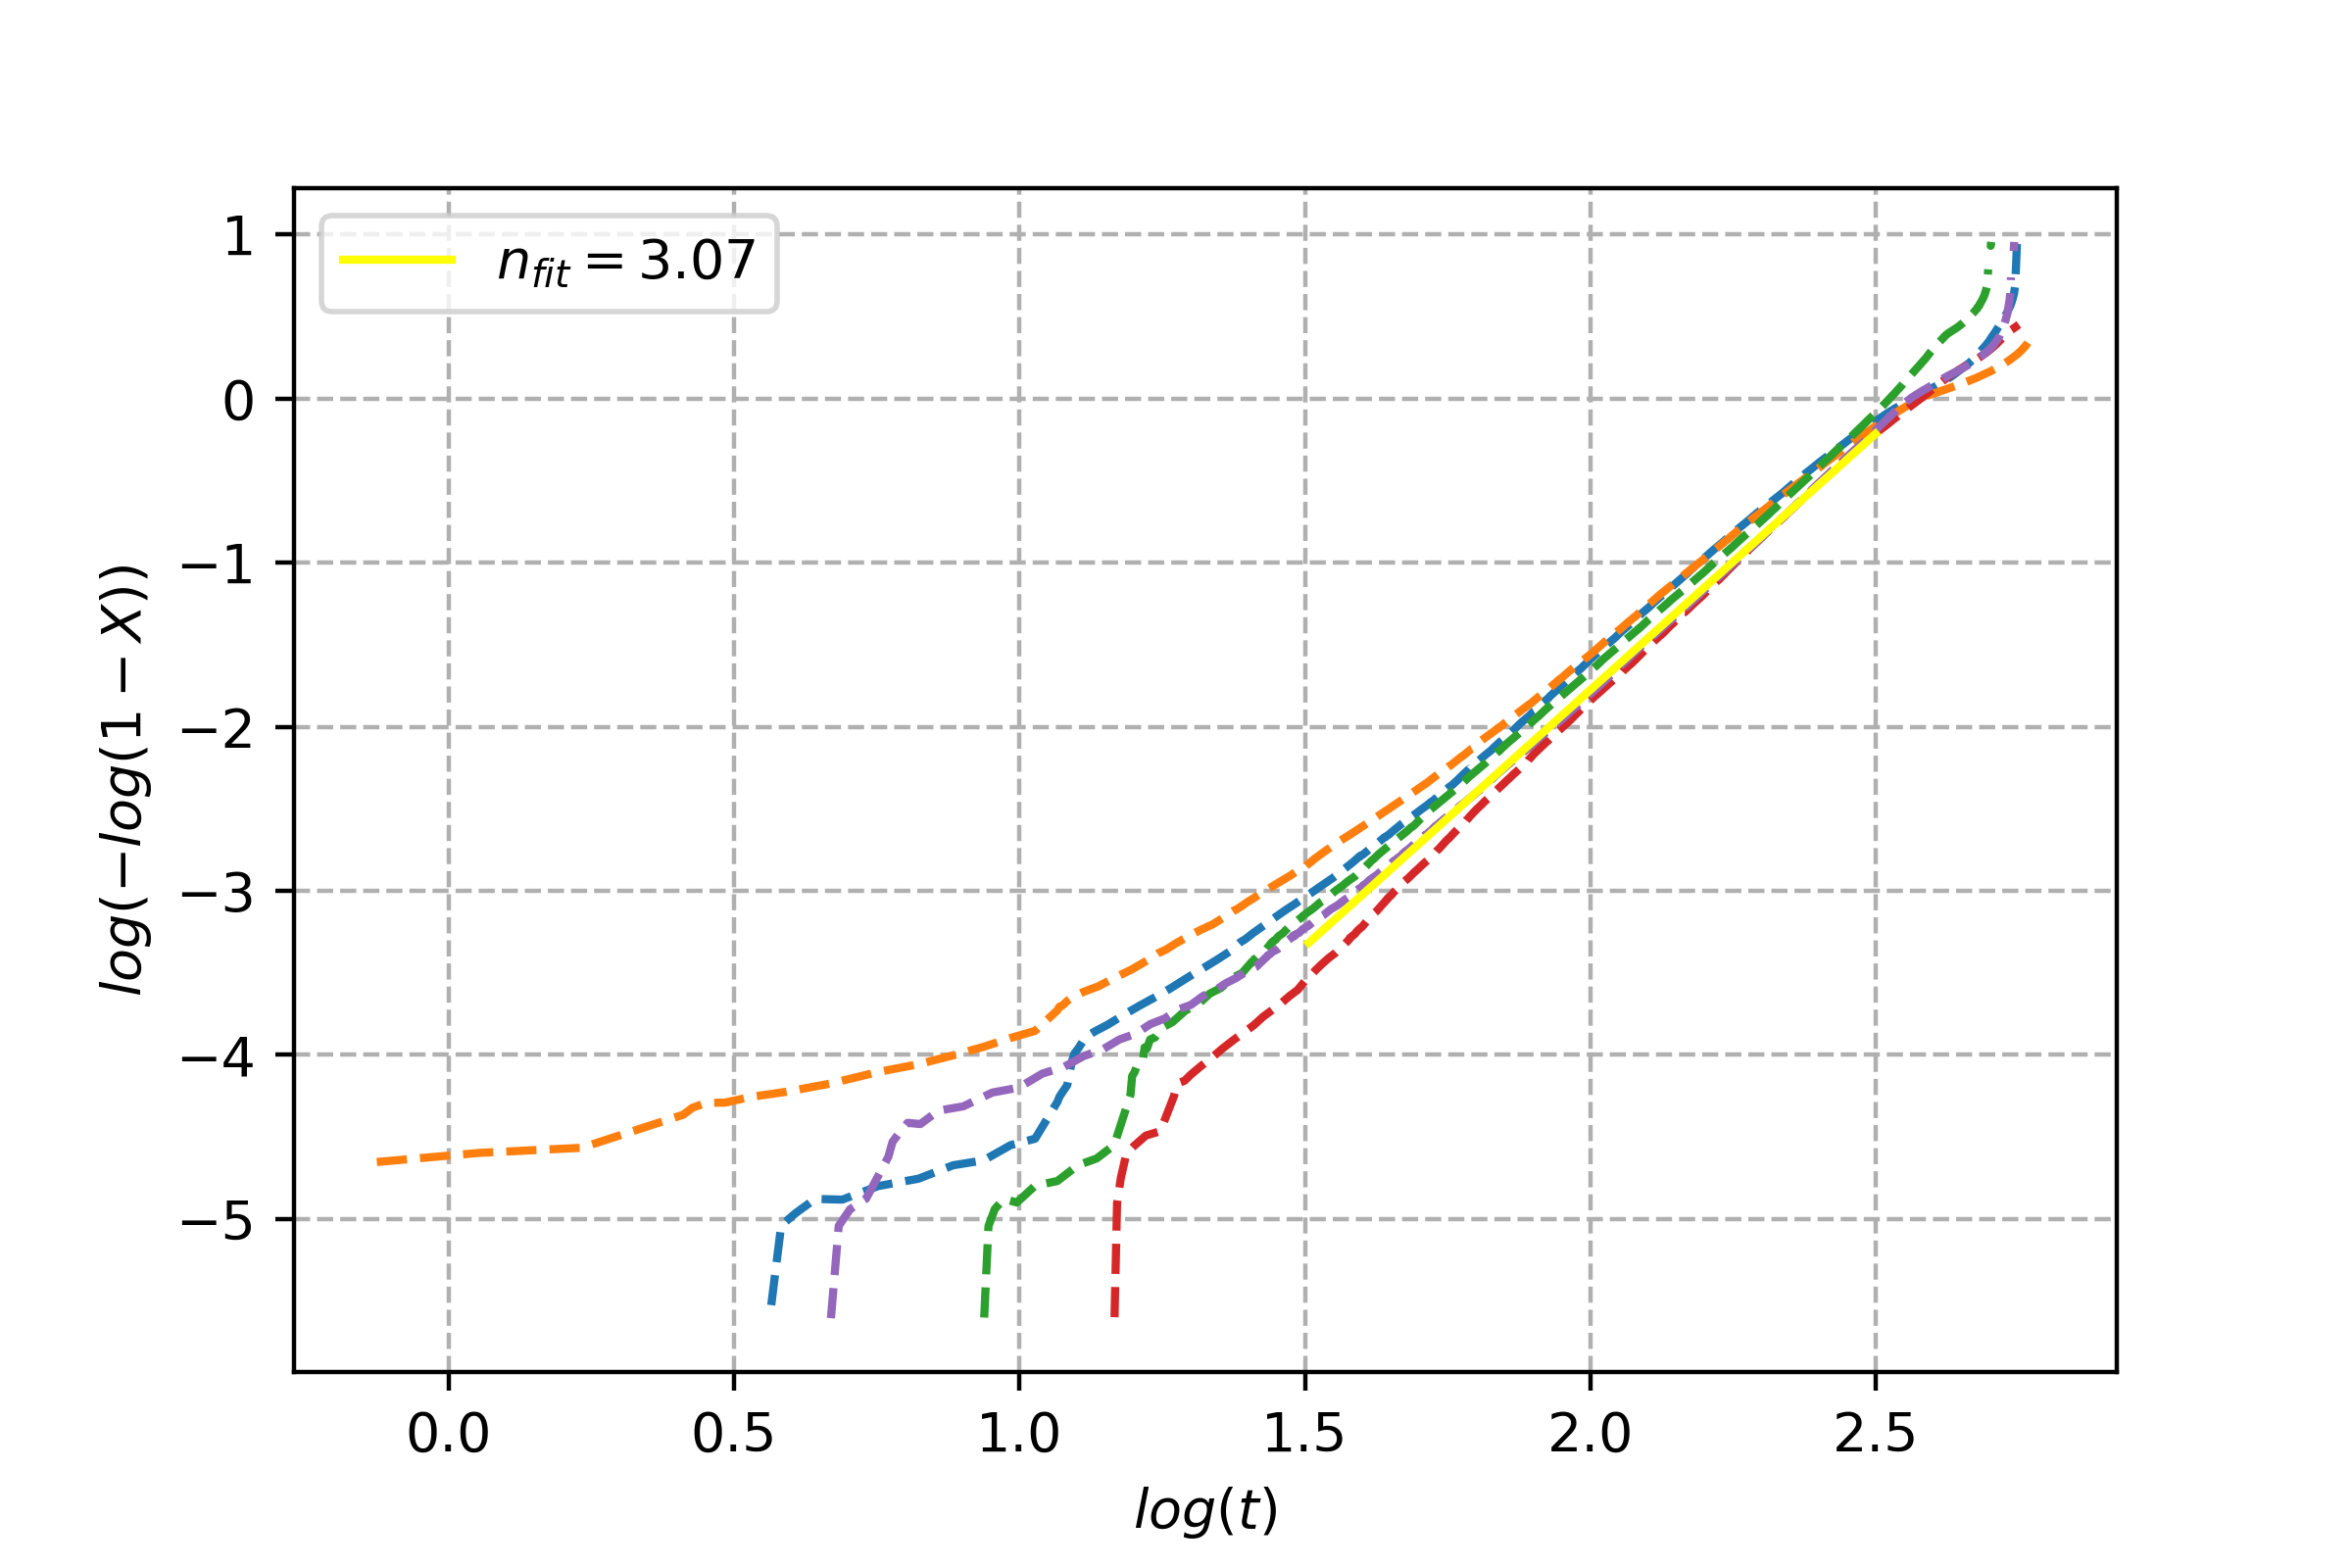
\includegraphics[scale=0.65]{Avrami_plot_multiple_seed_randt.PNG}
\par\end{centering}
\caption{The Avrami plots of the multiple seed homogeneous nucleation at random times. Only one of the five fitted slopes is shown.} \label{fig:avarmi_plot_multiple_seed_randt}
\end{figure}
\par\end{center}
%
\begin{center}
\begin{figure} 
\begin{centering}
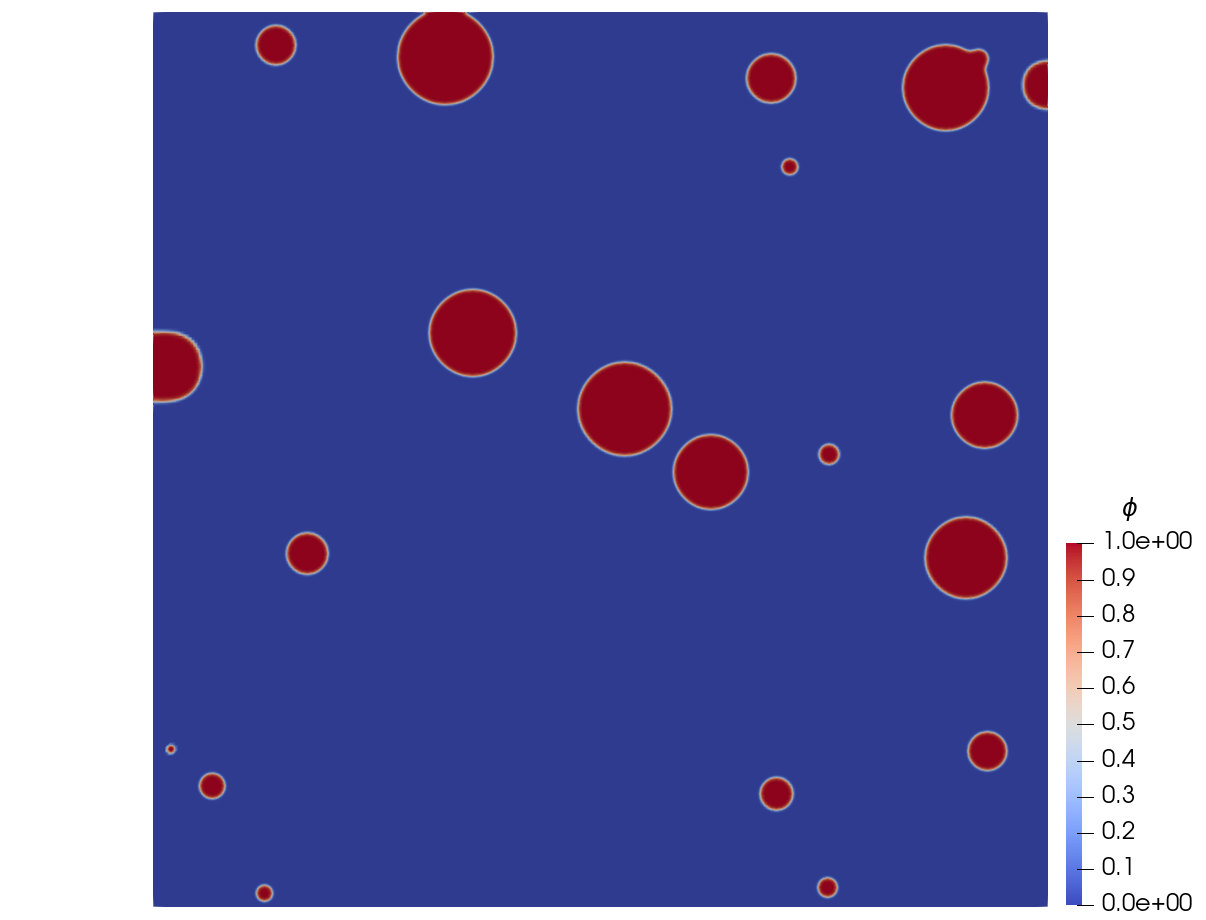
\includegraphics[scale=0.80]{t100_multiple_seed_randt.PNG}
\par\end{centering}
\caption{Snapshot of the phase-field domain at $t=100$.} \label{fig:t100_multiple_seed_randt}
\end{figure}
\par\end{center}

\subsection{Athermal heterogeneous nucleation}

In this benchmark problem we study how the driving force for solidification influences the free-growth condition of athermal heterogeneous nucleation. Figure~\ref{fig:snapshot_athermal} shows what the system looks like at $t=6500$ under different driving forces. %{\bf Olle: would need this in the problem statement} The main metric for comparing results for the different applied undercooling, the solid fraction, is shown in Fig.~\ref{fig:solid_fraction_athermal}.
%solid fraction is used as the metrics to compare simulation results {\bf Olle: the solid fraction as a metric should be in the problem statement (Fig.~\ref{fig:solid_fraction_athermal}). 

When the applied undercooling driving force $\Delta f=1.00\Delta f_0$, the particle will reach its free growth limit, which is the half-circular configuration, and its radius is equal to the radius of the homogeneous nucleus corresponding to the given driving force.  When $\Delta f=.098\Delta f_0$, the corresponding critical radius increases, the newly formed nucleus on the surface cannot grow freely, its final shape could be treated as part of a circle with larger radius compared to the previous case. The solid fraction of these two cases increases at the beginning but would reach a plateau very soon (black solid line and red dashed line in Fig.~\ref{fig:solid_fraction_athermal}).  When we increase the undercooling driving force to $\Delta f=1.02\Delta f_0$, the corresponding critical radius decreases, the particle is able to grow freely and almost takes up the space of the entire system. The corresponding solid fraction would keep increasing until it becomes close to 1. We remark that the system is very sensitive to numerical errors around $\Delta f=1.00\Delta f_0$, for some methods, free growth cannot be observed when $\Delta f=1.02\Delta f_0$. Further increasing the driving force to $\Delta f=1.04\Delta f_0$ may help the free growth to occur. Unsurprisingly, for those methods that evidenced free growth at $\Delta f=1.02\Delta f_0$, a faster growth rate is observed when $\Delta f=1.04\Delta f_0$.

We have performed a convergence test for the solid fraction change for an undercooling driving force of $\Delta f=1.1\Delta f_0$, as shown in Fig.~\ref{fig:convergence_athermal}. %We choose $\Delta f=1.1\Delta f_0$ for the convergence test due to the same reason for the first problem. The system is too sensitive when $\Delta f$ is close to $\Delta f_0$, even small numerical errors could lead to big result differences. And we don't want to set $\Delta f$ too far from $\Delta f_0$ otherwise the convergence behavior would not be obvious. 
As we refined the mesh resolution from $\Delta x=0.4$ to $\Delta x=0.025$, the solid fraction curve would gradually shift to the right -- with decreasing mesh size, it takes longer for the solid fraction to grow. %The free growth would occur a little bit later with a finer resolution. 
Our L2 error at $t=800$ is 0.42 between mesh sizes of $\Delta x=0.05$ and $\Delta x=0.025$, the L2 error is 0.23 between mesh sizes of $\Delta x=0.025$ and $\Delta x=0.0125$.
%{\bf Olle: This is a bit weird: is the adaptive-mesh solution converged or not? There is also a difference between 0.05 and 0.025; how do you know that 0.025 is converged? Maybe you should do one more run with $\Delta x=0.0125$?} 
Figure ~\ref{fig:convergence_athermal} shows that visually, the difference between mesh size of $\Delta x=0.05$ and $\Delta x=0.025$ is already barely discernible. It is interesting to note that the result for a mesh size of $\Delta x=0.0125$ (not shown) is indistinguishable from using adaptive meshing -- and of course at least in our case the run-time for adaptive meshing was smaller by orders of magnitudes than the run-time for a fixed mesh with $\Delta x=0.0125$. 
%If we compare the solid fraction change of $\Delta x=0.05$ and $\Delta x=0.025$ case, the difference is really small. We could conclude that further increase of the mesh resolution beyond $\Delta x=0.025$ would not help improve the accuracy of the simulation results too much compared to the additional computational resources needed for finer resolution calculations. If we compare the $\Delta x=0.025$ case to the case that applies the adaptive mesh, unlike the convergence test for the first problem, although the finest part of the adaptive mesh also contains element with size of $\Delta x=0.025$, there is a noticeable difference between the solid fraction curves for the two cases. And this difference would be even more obvious when $\Delta f$ gets close to $\Delta f_0$. (REASON FOR THIS??)

%
\begin{center}
\begin{figure} 
\begin{centering}
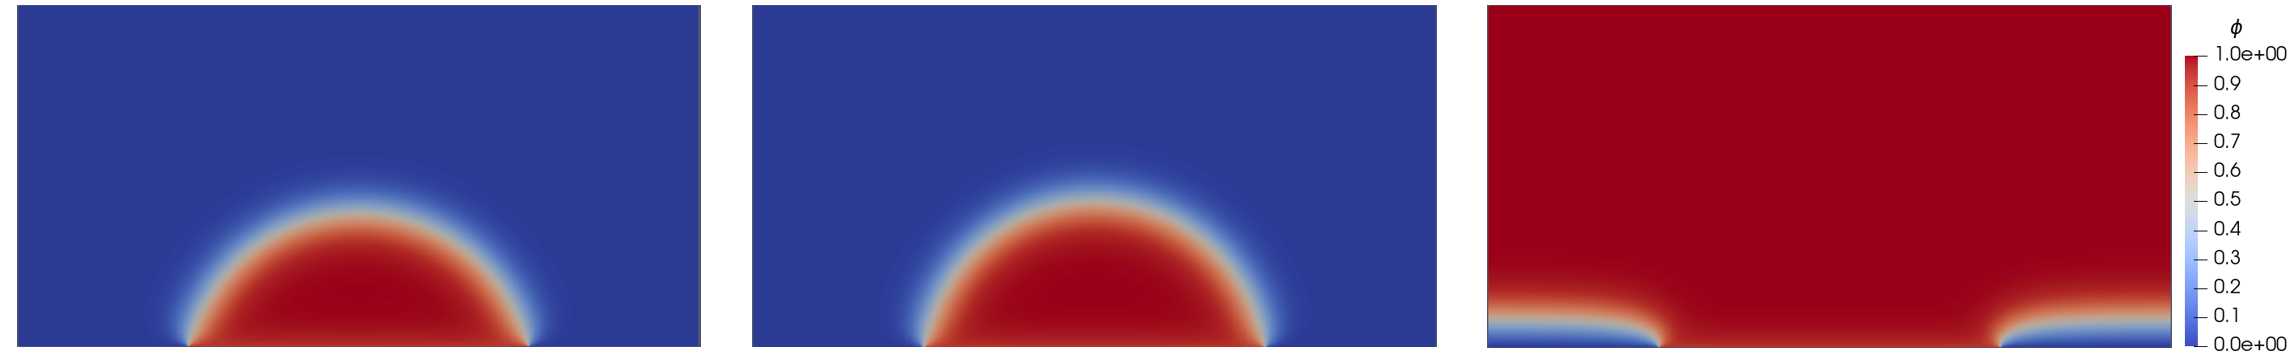
\includegraphics[scale=0.65]{snapshot_athermal.PNG}
\par\end{centering}
\caption{The snapshot for the athermal heterogeneous nucleation at $t=6500$ when (a) $\Delta f=0.98\Delta f_0$, (b) $\Delta f=1.00\Delta f_0$, (c) $\Delta f=1.02\Delta f_0$.} \label{fig:snapshot_athermal}
\end{figure}
\par\end{center}
%
%
\begin{center}
\begin{figure} 
\begin{centering}
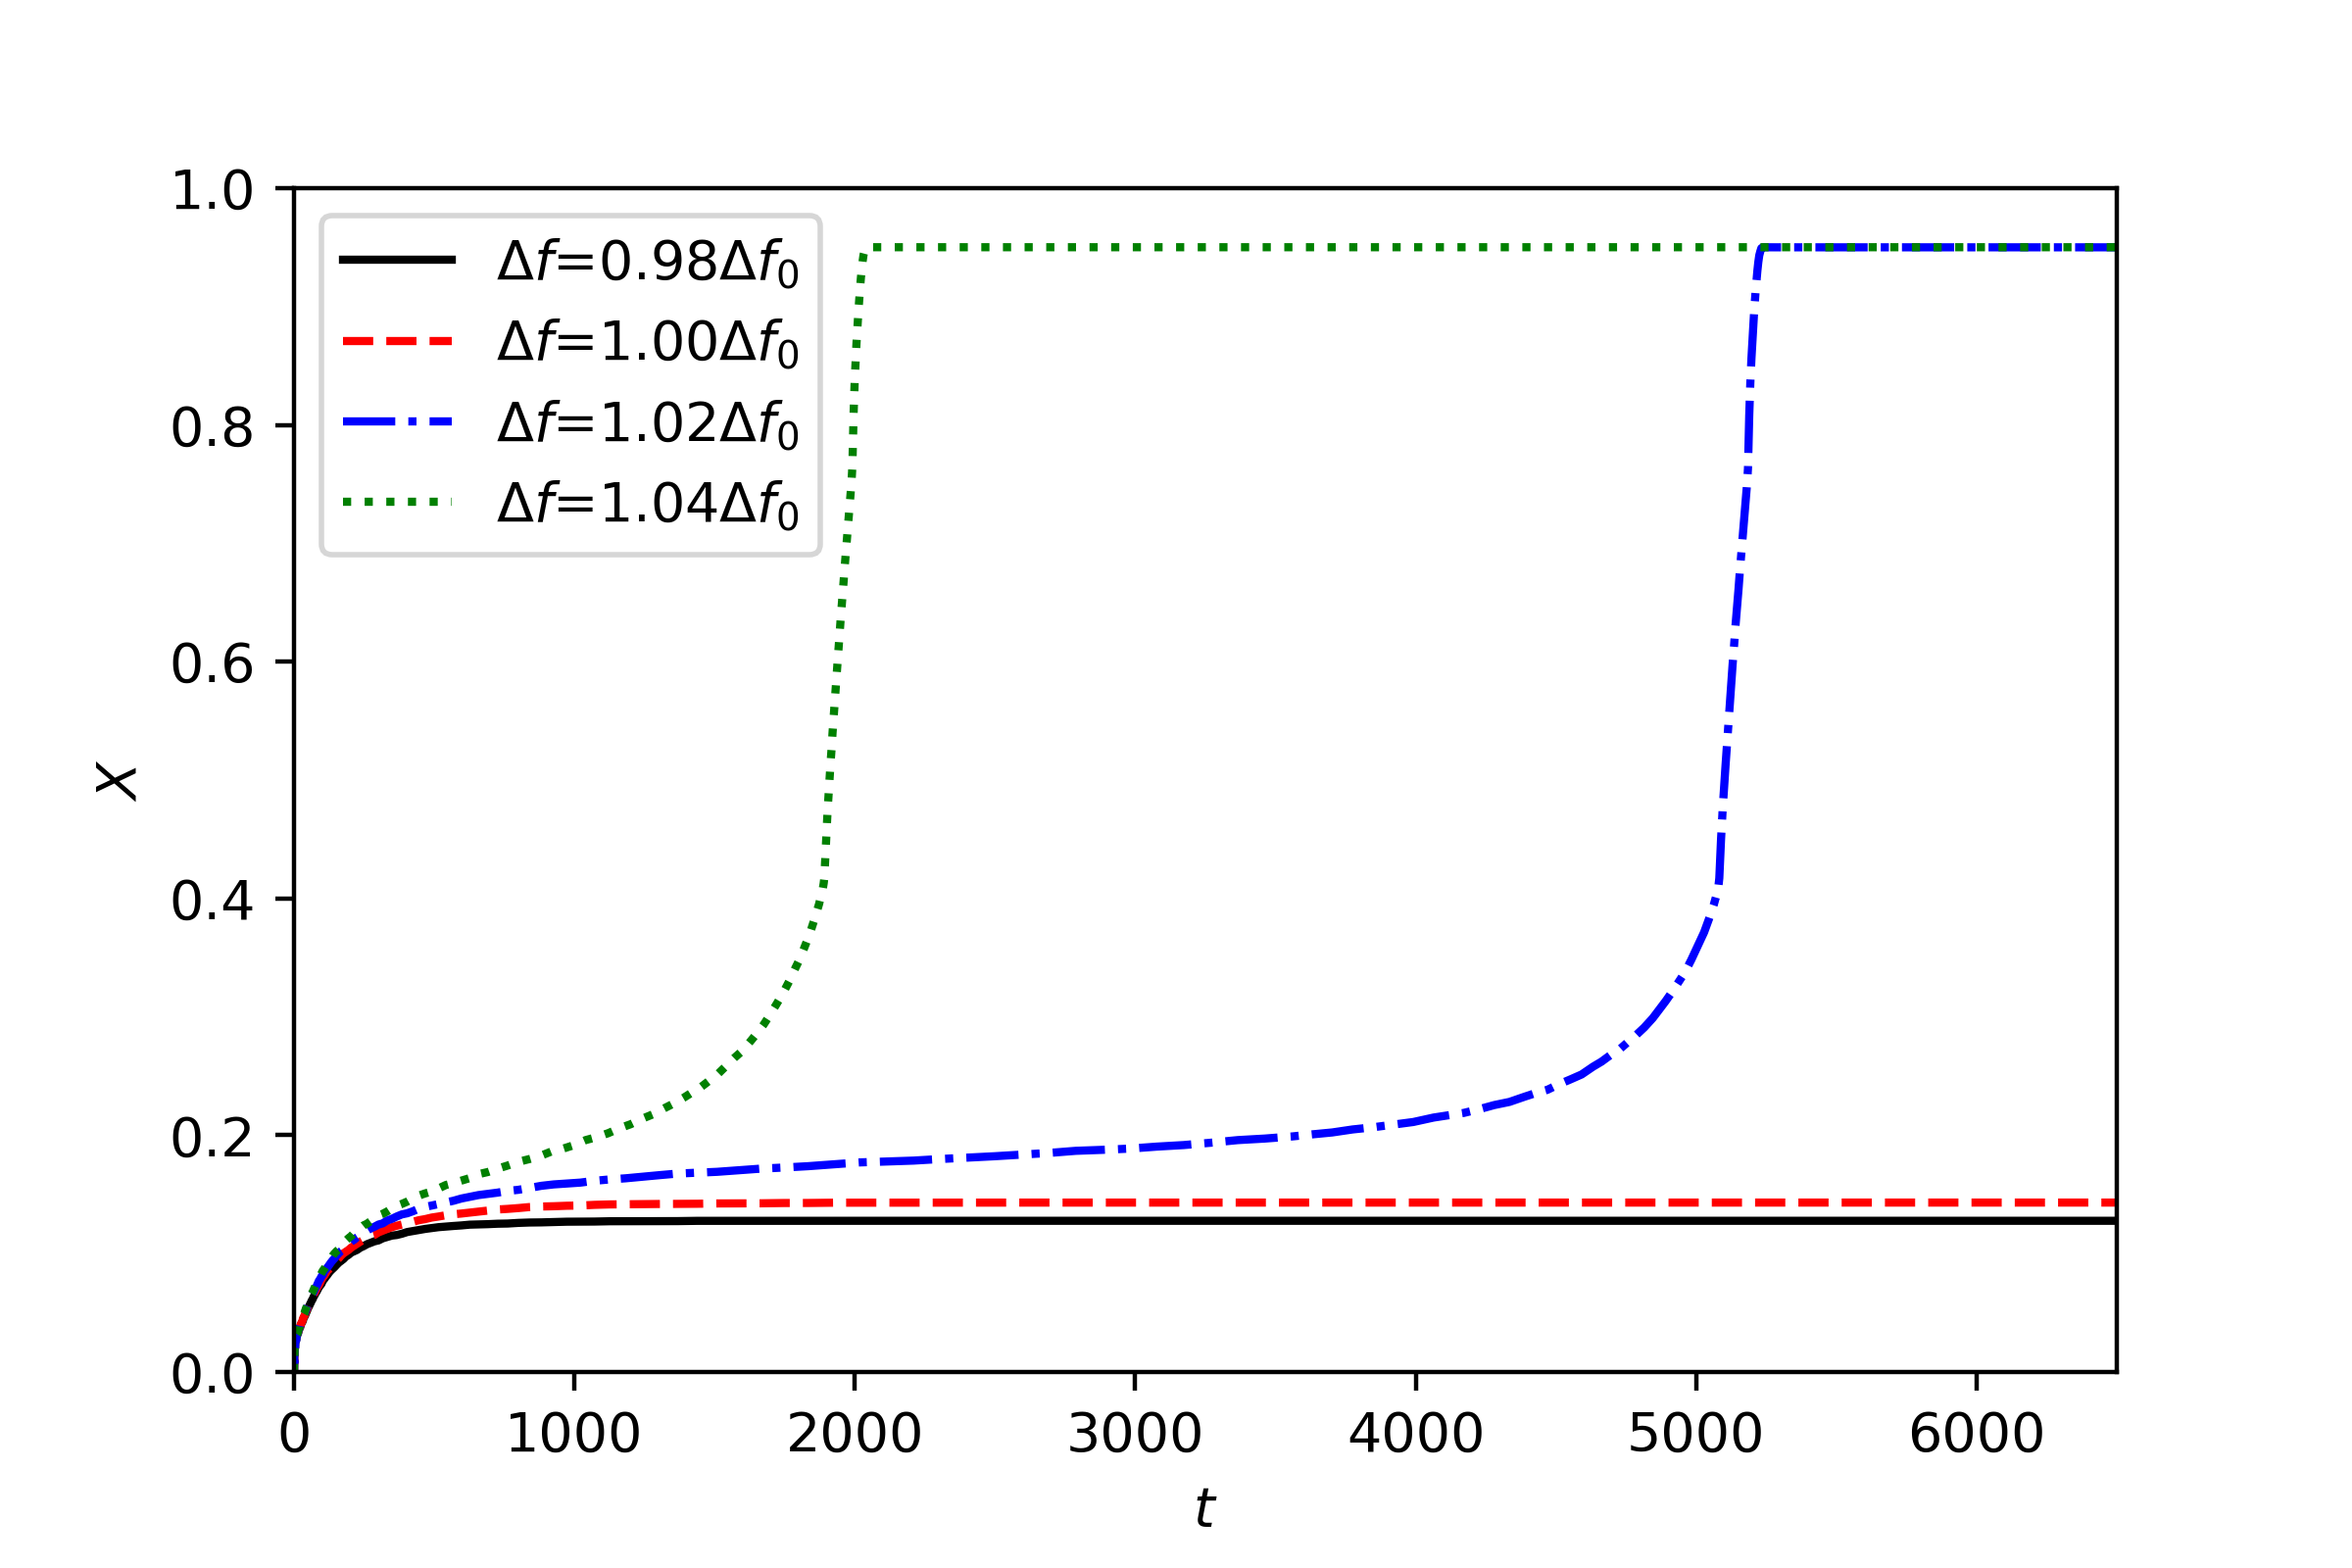
\includegraphics[scale=0.65]{solid_fraction_athermal.PNG}
\par\end{centering}
\caption{The solid fraction of the athermal heterogeneous nucleation for $\Delta f=0.98\Delta f_0$, $\Delta f=1.00\Delta f_0$, $\Delta f=1.02\Delta f_0$, and $\Delta f=1.04\Delta f_0$.} \label{fig:solid_fraction_athermal}
\end{figure}
\par\end{center}
%
%
\begin{center}
\begin{figure} 
\begin{centering}
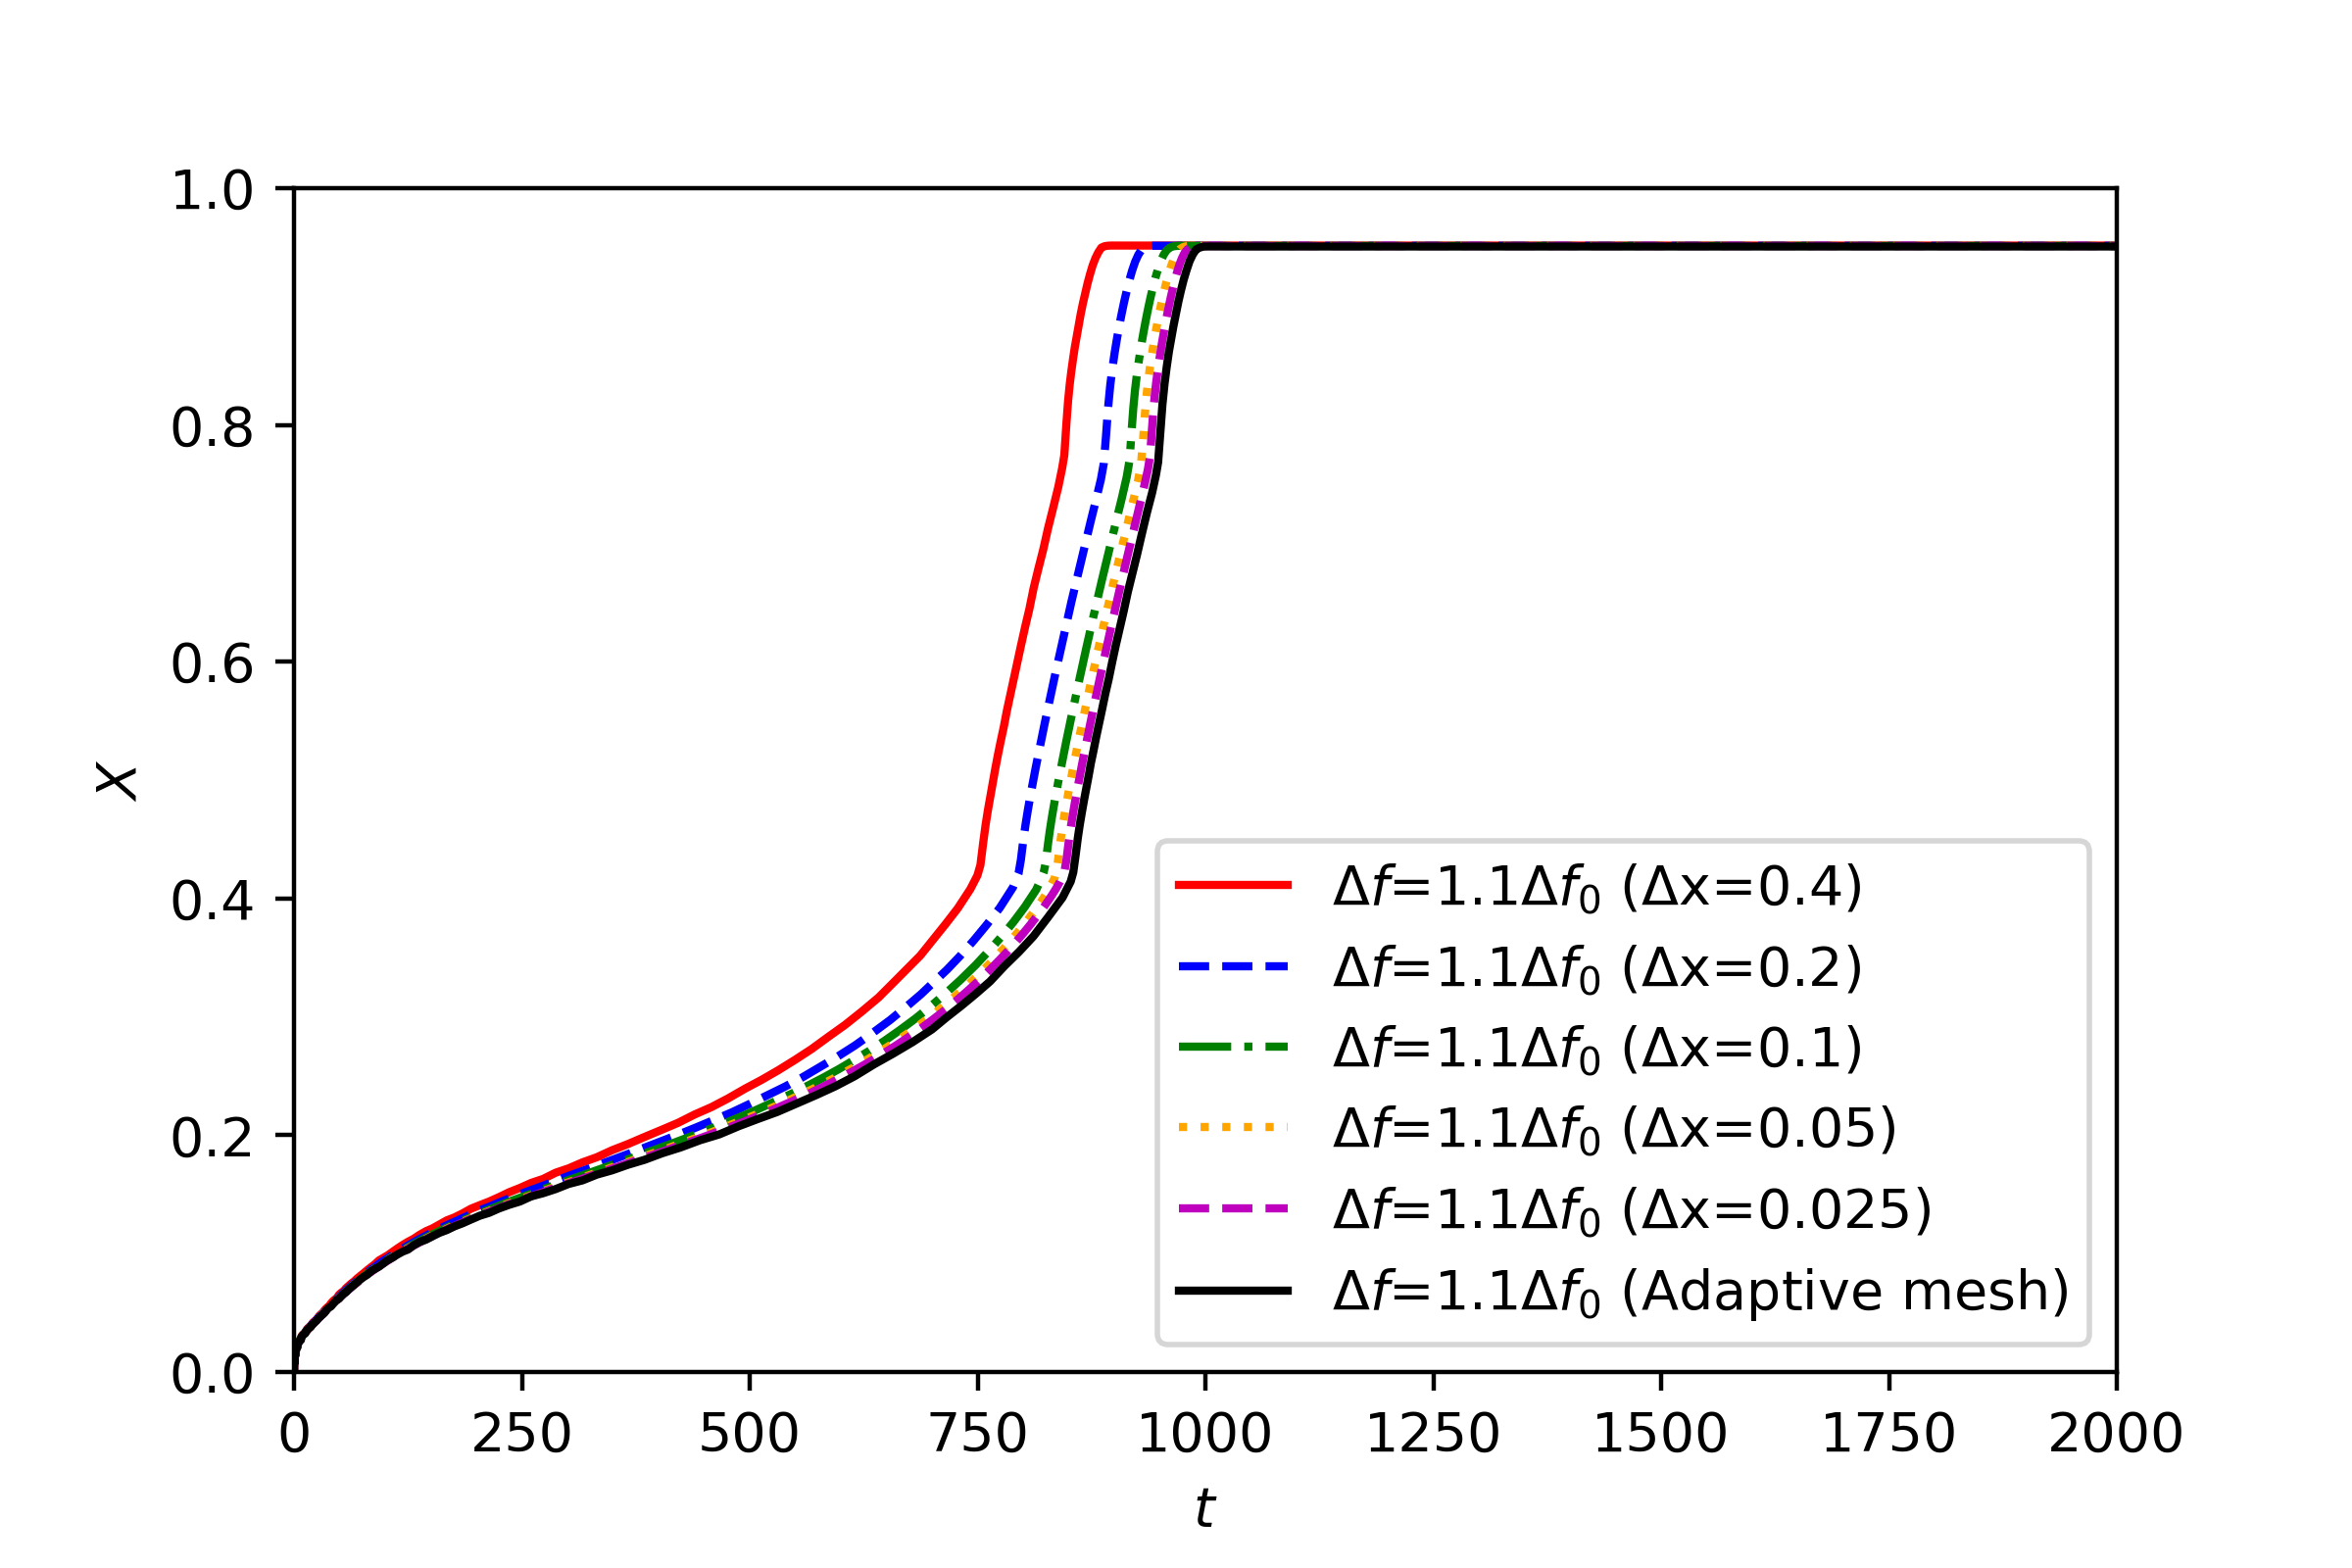
\includegraphics[scale=1.0]{convergence_athermal.PNG}
\par\end{centering}
\caption{The convergence test for the solid fraction change in the case $\Delta f=1.1\Delta f_0$.}\label{fig:convergence_athermal}
\end{figure}
\par\end{center}
%

\section{Conclusion}

The benchmark problems on homogeneous and heterogeneous nucleation presented in this work are an addition to our ongoing work to develop benchmark problems for phase field modeling~\cite{jokisaari2017spinodal,jokisaari2017dendrite,jokisaari2020stokes}. %Here, we expand the portfolio of benchmark problems to include four problems on nucleation. 
It is our hope that the discussions of these problems are of instructional value to practitioners, teachers, and students. %From the first problem it can be learned that the free energy increases as the particle grows when its initial radius is small and decreases when it is large beyond the critical radius. As a result, 
On a pedagogical level, the first problem illustrates that an initial particle will shrink and dissolve when its initial radius is smaller than the critical radius, and that it will grow when its initial radius is larger than the critical radius. The second and third parts of this problem provide simple illustrations of nucleation kinetics and connects the results to the JMAK theory. When the nucleation happens at $t=0$, the slope of the Avrami plot is about equal to $d$, where $d$ is the domain dimension. When the nucleation happens at random times, the slope of the Avrami plot is around $d+1$. The second problem demonstrates the free growth condition for the athermal heterogeneous nucleation. Free growth will only occur when the driving force of solidification is larger than the critical driving force corresponding to the critical radius. 

As benchmark problems aimed at probing numerical implementations, the problems highlight several potential issues. Numerical solutions are sensitive to any perturbations or numerical noise when initial radii are close to the critical radius $r^*$. This very evident in the first part of problem one (single-seed nucleation). Depending on the numerical implementation and the specific code, the solid fraction at an initial radius $r_0=r^*$ could either increase or diminish (Fig.~\ref{fig:solid_fraction_single_seed}). Similarly, for the athermal nucleation (problem two), different numerical implementations and codes may give different results close to critical driving force (Fig.~\ref{fig:solid_fraction_athermal}), with the steep onset of growth occurring at later or earlier times. 

A related issue is that when $r_0$ is close to $r^*$ in the single-seed homogeneous nucleation, or close to critical driving force in the single-seed athermal nucleation, the convergence with respect to mesh size can be slow and care has to be taken to ensure that the results are well converged with respect to mesh size. This is especially the case for the athermal nucleation close to critical driving ($\Delta f = 1.1 f_0$), where we had to reduce the mesh size to $\Delta x=0.025$ for well-converged solution. It is interesting -- and reassuring -- to note that in both cases, adaptive meshing led to well-converged solutions at much smaller execution time than for a fine uniform mesh. This clearly demonstrates the power of adaptive meshing schemes for these problems.

The slopes of the Avrami plots, especially for multiple seeds at $t=0$ typically are larger than the ideal value $d$. The reason for this is subtle: the JMAK model assumes circular particles, sometimes overlapping. At the points of overlap, there will be cusps in the boundary of the merged particles (see, {\em e.g.,}, Fig.~\ref{fig:t40_multiple_seed_t0}). Because the Cahn-Hilliard equations correctly incorporate the Gibbs-Thomson effect, the time-evolution of the systems seeks to smooth out cusps and make them straighter. This leads to a faster growth of the solid fraction than predicted by the JMAK theory. This is particularly evident at smaller driving forces where contributions to the free energy from the Gibbs-Thomson effect are relatively larger. We initially ran simulations for part two of problem one (multiple seeds at $t=0$) with a driving force $\Delta f=1/(6\sqrt{2})$. This resulted in slopes in the Avrami plots of close to 2.3. Increasing the driving force by a factor of 2 to $\Delta f=1/(3\sqrt{2})$ has the effect of decreasing the interfacial energy relative to the bulk free energy, which diminishes the Gibbs-Thomson effect and slows down the growth of the solid fraction so the slope in the Avrami plot approaches the ideal value. We confirmed that for the system sizes used here ($500\times500$), the slopes in the Avrami plots were not affected by finite-size effects. One the other hand, part three of problem one (multiple seeds at random times) gave slopes very close to the ideal value of $d+1$ without increasing the driving force from $\Delta f=1/(6\sqrt{2})$. We believe this is because the constant-rate nucleation yields a better average over microscopic processes that diminishes the effect of cusps. 

The development of these benchmark problems, as the ones before them, have relied very heavily on comments and feedback from the community. It is a great experience to work in this way with an enthusiastic and engaged community. In order to make these benchmark problems as useful as possible, we urge the community to continue to provide feedback for existing and possible additional benchmark problems at \url{https://pages.nist.gov/pfhub/}.

\section*{Acknowledgments}
This work was performed under financial assistance award 70NANB19H005 from U.S. Department of Commerce, National Institute of Standards and Technology as part of the Center for Hierarchical Material Design (CHiMaD). DM was supported by the U.S. Department of Energy, Office of Basic Energy Sciences, Division of Materials Sciences and Engineering under Award \#DE-SC0008637 as part of the Center for PRedictive Integrated Structural Materials Science (PRISMS Center) at University of Michigan. TP and LG were supported by the National Agency for Research, Development, and Innovation, Hungary (NKFIH contract no. KKP-126749). We gratefully acknowledge the computing resources provided on Bebop and Blues, high-performance computing clusters operated by the Laboratory Computing Resource Center at Argonne National Laboratory. We particularly thank the participants of the Phase Field Workshops held in Evanston, IL, to whom we are deeply indebted for invaluable feedback and comments.   

\bibliographystyle{model1-num-names}
\bibliography{NucleationBenchmark.bib}

\end{document}
